\documentclass[a4paper]{book}
\usepackage{makeidx}
\usepackage{natbib}
\usepackage{graphicx}
\usepackage{multicol}
\usepackage{float}
\usepackage{listings}
\usepackage{color}
\usepackage{ifthen}
\usepackage[table]{xcolor}
\usepackage{textcomp}
\usepackage{alltt}
\usepackage{ifpdf}
\ifpdf
\usepackage[pdftex,
            pagebackref=true,
            colorlinks=true,
            linkcolor=blue,
            unicode
           ]{hyperref}
\else
\usepackage[ps2pdf,
            pagebackref=true,
            colorlinks=true,
            linkcolor=blue,
            unicode
           ]{hyperref}
\usepackage{pspicture}
\fi
\usepackage[utf8]{inputenc}
\usepackage{mathptmx}
\usepackage[scaled=.90]{helvet}
\usepackage{courier}
\usepackage{sectsty}
\usepackage[titles]{tocloft}
\usepackage{doxygen}
\lstset{language=C++,inputencoding=utf8,basicstyle=\footnotesize,breaklines=true,breakatwhitespace=true,tabsize=8,numbers=left }
\makeindex
\setcounter{tocdepth}{3}
\renewcommand{\footrulewidth}{0.4pt}
\renewcommand{\familydefault}{\sfdefault}
\hfuzz=15pt
\setlength{\emergencystretch}{15pt}
\hbadness=750
\tolerance=750
\begin{document}
\hypersetup{pageanchor=false,citecolor=blue}
\begin{titlepage}
\vspace*{7cm}
\begin{center}
{\Large \-Roculus \\[1ex]\large 1.\-0 }\\
\vspace*{1cm}
{\large \-Generated by Doxygen 1.7.6.1}\\
\vspace*{0.5cm}
{\small Wed Aug 20 2014 16:10:06}\\
\end{center}
\end{titlepage}
\clearemptydoublepage
\pagenumbering{roman}
\tableofcontents
\clearemptydoublepage
\pagenumbering{arabic}
\hypersetup{pageanchor=true,citecolor=blue}
\chapter{\-Namespace \-Index}
\section{\-Namespace \-List}
\-Here is a list of all documented namespaces with brief descriptions\-:\begin{DoxyCompactList}
\item\contentsline{section}{\hyperlink{namespaceOVR}{\-O\-V\-R} }{\pageref{namespaceOVR}}{}
\end{DoxyCompactList}

\chapter{\-Class \-Index}
\section{\-Class \-Hierarchy}
\-This inheritance list is sorted roughly, but not completely, alphabetically\-:\begin{DoxyCompactList}
\item \contentsline{section}{\-Base\-Application}{\pageref{classBaseApplication}}{}
\begin{DoxyCompactList}
\item \contentsline{section}{\-Roculus}{\pageref{classRoculus}}{}
\end{DoxyCompactList}
\item \contentsline{section}{\-Game}{\pageref{classGame}}{}
\item \contentsline{section}{\-Game\-C\-F\-G\-Parser}{\pageref{classGameCFGParser}}{}
\item \contentsline{section}{\-Game\-Object}{\pageref{classGameObject}}{}
\begin{DoxyCompactList}
\item \contentsline{section}{\-Door}{\pageref{classDoor}}{}
\item \contentsline{section}{\-Key}{\pageref{classKey}}{}
\item \contentsline{section}{\-Lock}{\pageref{classLock}}{}
\item \contentsline{section}{\-Treasure}{\pageref{classTreasure}}{}
\end{DoxyCompactList}
\item \contentsline{section}{\-Global\-Map}{\pageref{classGlobalMap}}{}
\item \contentsline{section}{\-Oculus}{\pageref{classOculus}}{}
\item \contentsline{section}{\-Player\-Body}{\pageref{classPlayerBody}}{}
\item \contentsline{section}{\-Robot}{\pageref{classRobot}}{}
\item \contentsline{section}{\-Room}{\pageref{classRoom}}{}
\item \contentsline{section}{\-Snapshot}{\pageref{classSnapshot}}{}
\item \contentsline{section}{\-Snapshot\-Library}{\pageref{classSnapshotLibrary}}{}
\item \contentsline{section}{\-Video3\-D}{\pageref{classVideo3D}}{}
\item \contentsline{section}{\-Way\-Point}{\pageref{classWayPoint}}{}
\end{DoxyCompactList}

\chapter{\-Class \-Index}
\section{\-Class \-List}
\-Here are the classes, structs, unions and interfaces with brief descriptions\-:\begin{DoxyCompactList}
\item\contentsline{section}{\hyperlink{classBaseApplication}{\-Base\-Application} \\*\-Ogre \hyperlink{classBaseApplication}{\-Base\-Application} class \-The \hyperlink{classBaseApplication}{\-Base\-Application} class is the central class in the project. \-It brings all systems together\-: $\ast$initialization and control of the rendering process $\ast$handling keyboard/mouse input $\ast$connection to \-R\-O\-S for joystick input, image sensor data, waypoint data, etc. $\ast$cleaning up after the application finished }{\pageref{classBaseApplication}}{}
\item\contentsline{section}{\hyperlink{classDoor}{\-Door} \\*\-Represents a \hyperlink{classDoor}{\-Door} in the demo-\/game. \-A door is a \hyperlink{classGameObject}{\-Game\-Object} and takes care of the appearance, as well as the behaviour of a door }{\pageref{classDoor}}{}
\item\contentsline{section}{\hyperlink{classGame}{\-Game} \\*\-Singleton pattern class to manage the demo-\/game. \-This class manages the demo-\/game and is responsible for all related objects, their (repeatable) initialization and the game process }{\pageref{classGame}}{}
\item\contentsline{section}{\hyperlink{classGameCFGParser}{\-Game\-C\-F\-G\-Parser} \\*\-Parses the 'game.\-cfg' file. \-This class provides an easy-\/to-\/use parser for the config file of a game. \-Note that the filename is hardcoded in the constructor }{\pageref{classGameCFGParser}}{}
\item\contentsline{section}{\hyperlink{classGameObject}{\-Game\-Object} \\*\-Describes a generic game object. \-This class is an abstract description of a game object. \-It give some default functionality and is otherwise used to inherit the properties to its child classes\-: \hyperlink{classDoor}{\-Door}, \hyperlink{classKey}{\-Key}, \hyperlink{classTreasure}{\-Treasure} and \hyperlink{classLock}{\-Lock} }{\pageref{classGameObject}}{}
\item\contentsline{section}{\hyperlink{classGlobalMap}{\-Global\-Map} \\*\-Utility class for the 2\-D map. \-This class handles the 2\-D map in the scene }{\pageref{classGlobalMap}}{}
\item\contentsline{section}{\hyperlink{classKey}{\-Key} \\*\-Represents a \hyperlink{classKey}{\-Key} in a \hyperlink{classGame}{\-Game}. \-This class is a more detailed description of the \hyperlink{classGameObject}{\-Game\-Object} \hyperlink{classKey}{\-Key}. \-It specifies how to display and what to do with a key }{\pageref{classKey}}{}
\item\contentsline{section}{\hyperlink{classLock}{\-Lock} \\*\-Describes a \hyperlink{classLock}{\-Lock} in a \hyperlink{classGame}{\-Game}. \-This class specifies the details to display a lock and implements its behaviour }{\pageref{classLock}}{}
\item\contentsline{section}{\hyperlink{classOculus}{\-Oculus} \\*\-Handler for the \hyperlink{classOculus}{\-Oculus} \-Rift using \-S\-D\-K1. \-Written by \-Kojack 2013 (\-C). \-Slightly modified to take the \-Plaber\-Body scene node as parent to the camera setup }{\pageref{classOculus}}{}
\item\contentsline{section}{\hyperlink{classPlayerBody}{\-Player\-Body} \\*\-Handles the \hyperlink{classPlayerBody}{\-Player\-Body} motion. \-Extension class to handle the player motion independent from the \hyperlink{classOculus}{\-Oculus} \-Rift head motion. \-The \hyperlink{classOculus}{\-Oculus} motion happens on top of this, which is achieved by making the \hyperlink{classPlayerBody}{\-Player\-Body}'s scene node the parent for the \hyperlink{classOculus}{\-Oculus} handler. \-Since this was one of my first implementations (very unclean) this step, in fact, happens in \hyperlink{classBaseApplication}{\-Base\-Application} }{\pageref{classPlayerBody}}{}
\item\contentsline{section}{\hyperlink{classRobot}{\-Robot} \\*\-Represents a \hyperlink{classRobot}{\-Robot}. \-This class handles the robot avatar }{\pageref{classRobot}}{}
\item\contentsline{section}{\hyperlink{classRoculus}{\-Roculus} \\*\-Class to take care of the scene and object creation. \-This class fills the scene with objects and in most cases creates the geometries manually. \-It has a method to parse room recordings in folders in order to include them into the scene. \-Though it is the nominal main class, the majority of the implementation is found in the \hyperlink{classBaseApplication}{\-Base\-Application} class }{\pageref{classRoculus}}{}
\item\contentsline{section}{\hyperlink{classRoom}{\-Room} \\*\-Describes a \hyperlink{classRoom}{\-Room} in a \hyperlink{classGame}{\-Game}. \-This class collects all parameters for a \hyperlink{classRoom}{\-Room}. \-It keeps track of the corresponding \-Way\-Points, \hyperlink{classDoor}{\-Door} nodes and event nodes and provides some utility functions }{\pageref{classRoom}}{}
\item\contentsline{section}{\hyperlink{classSnapshot}{\-Snapshot} \\*\-Collects all data that describes a \hyperlink{classSnapshot}{\-Snapshot} and provides a method to insert it into the scene. (\-Not the smartest implementation, should probably be constructed given the scene manager and do the object creation by itself. \-Static counter would help to identify total number of \-Snapshots to link to individual materials, textures etc.) }{\pageref{classSnapshot}}{}
\item\contentsline{section}{\hyperlink{classSnapshotLibrary}{\-Snapshot\-Library} \\*\-Groups multiple \-Snapshots in a library (vector). \-Furthermore, this class manages the memory and preallocates \-Ogre\-::\-Textures, \-Materials and \-Scene\-Nodes, whenever needed }{\pageref{classSnapshotLibrary}}{}
\item\contentsline{section}{\hyperlink{classTreasure}{\-Treasure} \\*\-Describes the appearance and behaviour of a \hyperlink{classTreasure}{\-Treasure} in the \hyperlink{classGame}{\-Game}. \-This class is similar to the other \-Game\-Objects }{\pageref{classTreasure}}{}
\item\contentsline{section}{\hyperlink{classVideo3D}{\-Video3\-D} \\*\-Handles the 3\-D video stream. \-Similar to a \hyperlink{classSnapshot}{\-Snapshot}, but uses \-D\-Y\-N\-A\-M\-I\-C and \-D\-I\-S\-C\-A\-R\-D\-A\-B\-L\-E textures instead, which are updated, not placed. (\-Not the smartest implementation, should probably be inherit properties from \hyperlink{classSnapshot}{\-Snapshot}...) }{\pageref{classVideo3D}}{}
\item\contentsline{section}{\hyperlink{classWayPoint}{\-Way\-Point} \\*\-Defines a \hyperlink{classWayPoint}{\-Way\-Point} for the \hyperlink{classGame}{\-Game}. \-Waypoints are possible navigation targets and are used to place \-Game\-Objects, like \-Keys and \-Locks. \-The list of \-Way\-Points is held by the \hyperlink{classGame}{\-Game} class, but they are read from other classes quite often, usually passed as a pointer or reference. \-A \hyperlink{classWayPoint}{\-Way\-Point} can be made inaccessible for the selection by the player setting the accessible flag }{\pageref{classWayPoint}}{}
\end{DoxyCompactList}

\chapter{\-Namespace \-Documentation}
\hypertarget{namespaceOVR}{\section{\-O\-V\-R \-Namespace \-Reference}
\label{namespaceOVR}\index{\-O\-V\-R@{\-O\-V\-R}}
}


\subsection{\-Detailed \-Description}
\-Copyright (\-C) 2013 \-Kojack

\-Permission is hereby granted, free of charge, to any person obtaining a copy of this software and associated documentation files (the \char`\"{}\-Software\char`\"{}), to deal in the \-Software without restriction, including without limitation the rights to use, copy, modify, merge, publish, distribute, sublicense, and/or sell copies of the \-Software, and to permit persons to whom the \-Software is furnished to do so, subject to the following conditions\-:

\-The above copyright notice and this permission notice shall be included in all copies or substantial portions of the \-Software.

\-T\-H\-E \-S\-O\-F\-T\-W\-A\-R\-E \-I\-S \-P\-R\-O\-V\-I\-D\-E\-D \char`\"{}\-A\-S I\-S\char`\"{}, \-W\-I\-T\-H\-O\-U\-T \-W\-A\-R\-R\-A\-N\-T\-Y \-O\-F \-A\-N\-Y \-K\-I\-N\-D, \-E\-X\-P\-R\-E\-S\-S \-O\-R \-I\-M\-P\-L\-I\-E\-D, \-I\-N\-C\-L\-U\-D\-I\-N\-G \-B\-U\-T \-N\-O\-T \-L\-I\-M\-I\-T\-E\-D \-T\-O \-T\-H\-E \-W\-A\-R\-R\-A\-N\-T\-I\-E\-S \-O\-F \-M\-E\-R\-C\-H\-A\-N\-T\-A\-B\-I\-L\-I\-T\-Y, \-F\-I\-T\-N\-E\-S\-S \-F\-O\-R \-A \-P\-A\-R\-T\-I\-C\-U\-L\-A\-R \-P\-U\-R\-P\-O\-S\-E \-A\-N\-D \-N\-O\-N\-I\-N\-F\-R\-I\-N\-G\-E\-M\-E\-N\-T. \-I\-N \-N\-O \-E\-V\-E\-N\-T \-S\-H\-A\-L\-L \-T\-H\-E \-A\-U\-T\-H\-O\-R\-S \-O\-R \-C\-O\-P\-Y\-R\-I\-G\-H\-T \-H\-O\-L\-D\-E\-R\-S \-B\-E \-L\-I\-A\-B\-L\-E \-F\-O\-R \-A\-N\-Y \-C\-L\-A\-I\-M, \-D\-A\-M\-A\-G\-E\-S \-O\-R \-O\-T\-H\-E\-R \-L\-I\-A\-B\-I\-L\-I\-T\-Y, \-W\-H\-E\-T\-H\-E\-R \-I\-N \-A\-N \-A\-C\-T\-I\-O\-N \-O\-F \-C\-O\-N\-T\-R\-A\-C\-T, \-T\-O\-R\-T \-O\-R \-O\-T\-H\-E\-R\-W\-I\-S\-E, \-A\-R\-I\-S\-I\-N\-G \-F\-R\-O\-M, \-O\-U\-T \-O\-F \-O\-R \-I\-N \-C\-O\-N\-N\-E\-C\-T\-I\-O\-N \-W\-I\-T\-H \-T\-H\-E \-S\-O\-F\-T\-W\-A\-R\-E \-O\-R \-T\-H\-E \-U\-S\-E \-O\-R \-O\-T\-H\-E\-R \-D\-E\-A\-L\-I\-N\-G\-S \-I\-N \-T\-H\-E \-S\-O\-F\-T\-W\-A\-R\-E. 
\chapter{\-Class \-Documentation}
\hypertarget{classBaseApplication}{\section{\-Base\-Application \-Class \-Reference}
\label{classBaseApplication}\index{\-Base\-Application@{\-Base\-Application}}
}


\-Ogre \hyperlink{classBaseApplication}{\-Base\-Application} class \-The \hyperlink{classBaseApplication}{\-Base\-Application} class is the central class in the project. \-It brings all systems together\-: $\ast$initialization and control of the rendering process $\ast$handling keyboard/mouse input $\ast$connection to \-R\-O\-S for joystick input, image sensor data, waypoint data, etc. $\ast$cleaning up after the application finished.  




{\ttfamily \#include $<$\-Base\-Application.\-h$>$}

\-Inheritance diagram for \-Base\-Application\-:\begin{figure}[H]
\begin{center}
\leavevmode
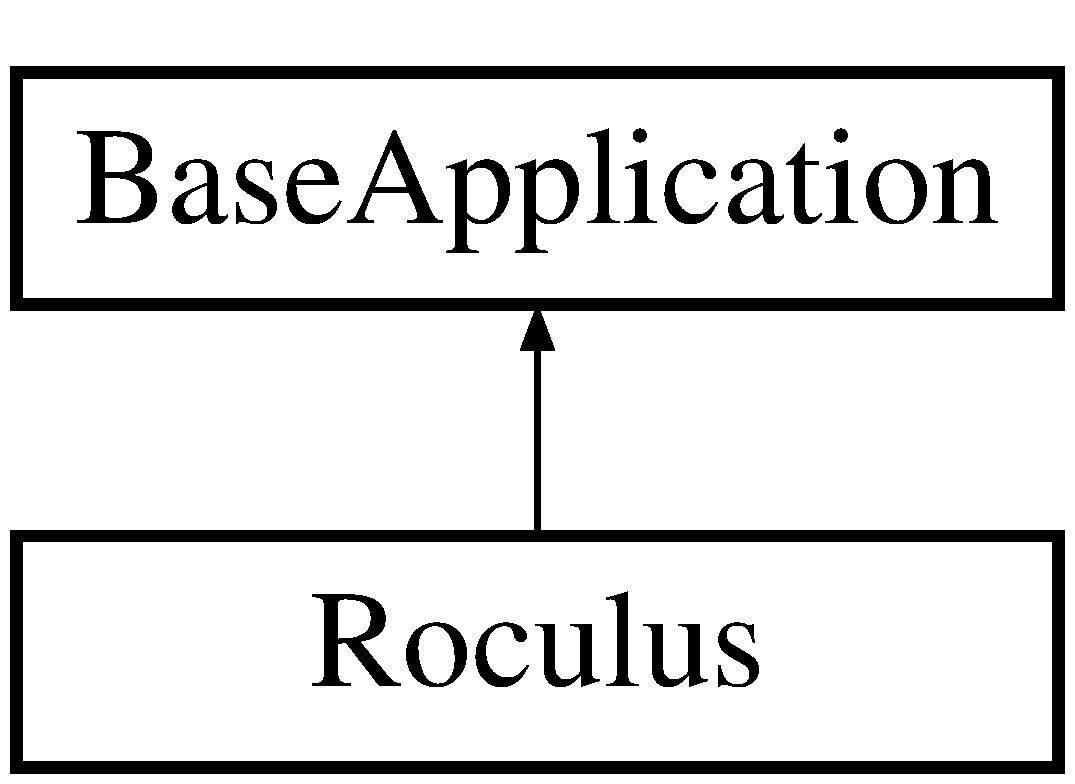
\includegraphics[height=2.000000cm]{classBaseApplication}
\end{center}
\end{figure}
\subsection*{\-Public \-Member \-Functions}
\begin{DoxyCompactItemize}
\item 
\hyperlink{classBaseApplication_a7c897f08816cc064568ae1ec71026719}{\-Base\-Application} (void)
\item 
virtual \hyperlink{classBaseApplication_a39133f736b9eb70263cebaca3e6d2cad}{$\sim$\-Base\-Application} (void)
\item 
virtual void \hyperlink{classBaseApplication_aed497661d1817ed9d659fb4de671ac1c}{go} (void)
\end{DoxyCompactItemize}
\subsection*{\-Protected \-Member \-Functions}
\begin{DoxyCompactItemize}
\item 
virtual bool \hyperlink{classBaseApplication_ae548b5e3ac0cf92d4dc7d478a8f01922}{setup} ()
\item 
virtual bool \hyperlink{classBaseApplication_a7882a8f2e08e8d6cde00e8c29b2153b0}{configure} (void)
\item 
virtual void \hyperlink{classBaseApplication_a0cf5e311b1c7426590ad6831e4c5352a}{choose\-Scene\-Manager} (void)
\item 
virtual void \hyperlink{classBaseApplication_ab672d2b969b8530ee753f8b000d219c6}{create\-Frame\-Listener} (void)
\item 
virtual void \hyperlink{classBaseApplication_aa97beeb4059b17d0ec22eae33286ec2d}{create\-Scene} (void)=0
\item 
virtual void \hyperlink{classBaseApplication_ab61c91a38b99f98ff369ce8098a91133}{destroy\-Scene} (void)
\item 
virtual void \hyperlink{classBaseApplication_aa71428aeca821504352f5f795e6a9226}{setup\-Resources} (void)
\item 
virtual void \hyperlink{classBaseApplication_a9e916d51e4d73e355091d0662c175d85}{create\-Resource\-Listener} (void)
\item 
virtual void \hyperlink{classBaseApplication_a7d72de4f9e3d17ce0a4a034d780baf67}{load\-Resources} (void)
\item 
virtual bool \hyperlink{classBaseApplication_af6c816b6ea18980a887d9fc92179f33b}{frame\-Started} (const \-Ogre\-::\-Frame\-Event \&evt)
\item 
virtual bool \hyperlink{classBaseApplication_adea8d433b93b66ec7ab48b7e244661df}{frame\-Rendering\-Queued} (const \-Ogre\-::\-Frame\-Event \&evt)
\item 
virtual bool \hyperlink{classBaseApplication_a0f1c9d085cafd1ead25cc8a85e944864}{frame\-Ended} (const \-Ogre\-::\-Frame\-Event \&evt)
\item 
virtual bool \hyperlink{classBaseApplication_ad79efa8c9d6f0f6a3cf8a34c25a1bd5f}{key\-Pressed} (const \-O\-I\-S\-::\-Key\-Event \&arg)
\item 
virtual bool \hyperlink{classBaseApplication_a72dbb7e590af8f96904bc55eb1875a56}{key\-Released} (const \-O\-I\-S\-::\-Key\-Event \&arg)
\item 
virtual bool \hyperlink{classBaseApplication_abbb67365fb496300701dc7a6953936fe}{mouse\-Moved} (const \-O\-I\-S\-::\-Mouse\-Event \&arg)
\item 
virtual bool \hyperlink{classBaseApplication_a51b515984916eb7a1582499ee3309ac5}{mouse\-Pressed} (const \-O\-I\-S\-::\-Mouse\-Event \&arg, \-O\-I\-S\-::\-Mouse\-Button\-I\-D id)
\item 
virtual bool \hyperlink{classBaseApplication_ae347f583327e4ba1eb83f2df286c1d76}{mouse\-Released} (const \-O\-I\-S\-::\-Mouse\-Event \&arg, \-O\-I\-S\-::\-Mouse\-Button\-I\-D id)
\item 
virtual void \hyperlink{classBaseApplication_ab5a43497cbab09b76cbe7a4708b7134f}{init\-R\-O\-S} ()
\item 
virtual void \hyperlink{classBaseApplication_ab51382d0741e40aa647e20a3315f84e8}{destroy\-R\-O\-S} ()
\item 
virtual void \hyperlink{classBaseApplication_a420db6b234d9201c678aea3bf32779b5}{joy\-Callback} (const sensor\-\_\-msgs\-::\-Joy\-::\-Const\-Ptr \&)
\item 
virtual void \hyperlink{classBaseApplication_a1b61407bd716b52034e43a53d6409267}{map\-Callback} (const nav\-\_\-msgs\-::\-Occupancy\-Grid\-::\-Const\-Ptr \&)
\item 
virtual void \hyperlink{classBaseApplication_a63abfe637034ac7f620ad62c57a9b899}{sync\-Video\-Callback} (const sensor\-\_\-msgs\-::\-Compressed\-Image\-Const\-Ptr \&, const sensor\-\_\-msgs\-::\-Compressed\-Image\-Const\-Ptr \&)
\item 
virtual void \hyperlink{classBaseApplication_a89d5c75390a28253d2ad3755334d9558}{topo\-Nodes\-C\-B} (const visualization\-\_\-msgs\-::\-Interactive\-Marker\-Init\-::\-Const\-Ptr \&)
\item 
virtual void \hyperlink{classBaseApplication_ac12e0269774652b57894b58ffdbfc4d5}{closest\-Way\-Point\-C\-B} (const std\-\_\-msgs\-::\-String\-::\-Const\-Ptr \&)
\item 
virtual void \hyperlink{classBaseApplication_afe5d7ca9e0f0575b4046c1412e314e69}{window\-Resized} (\-Ogre\-::\-Render\-Window $\ast$rw)
\item 
virtual void \hyperlink{classBaseApplication_aa7130c376136aa3a9b121e2dee561aed}{window\-Closed} (\-Ogre\-::\-Render\-Window $\ast$rw)
\end{DoxyCompactItemize}
\subsection*{\-Protected \-Attributes}
\begin{DoxyCompactItemize}
\item 
\-Ogre\-::\-Root $\ast$ \hyperlink{classBaseApplication_add84ba707dc6c57e6283f214b1274110}{m\-Root}
\item 
\-Ogre\-::\-Scene\-Manager $\ast$ \hyperlink{classBaseApplication_a8a7684f4f9a57ed3089048ad1a913b2d}{m\-Scene\-Mgr}
\item 
\-Ogre\-::\-Render\-Window $\ast$ \hyperlink{classBaseApplication_ac5d8e9c81e036897bc82f81eff8c570f}{m\-Window}
\item 
\-Ogre\-::\-String \hyperlink{classBaseApplication_a765e0df01c141a16df3178ab4f17afe6}{m\-Resources\-Cfg}
\item 
\-Ogre\-::\-String \hyperlink{classBaseApplication_a04f2fe47fa164fd78d986dc0df70b7fb}{m\-Plugins\-Cfg}
\item 
\-Ogre\-::\-Overlay\-System $\ast$ \hyperlink{classBaseApplication_a17ccdacc654eff8ac0d09f025311fbb5}{m\-Overlay\-System}
\item 
\-Ogre\-Bites\-::\-Input\-Context \hyperlink{classBaseApplication_a7da63f46f2ccf2c6385723c11c03301f}{m\-Input\-Context}
\item 
\-Ogre\-Bites\-::\-Sdk\-Tray\-Manager $\ast$ \hyperlink{classBaseApplication_a7faa397f4f4861ee8c361a01e90b4416}{m\-Tray\-Mgr}
\item 
\-Ogre\-Bites\-::\-Params\-Panel $\ast$ \hyperlink{classBaseApplication_a6a11054ca61efdf558e0ff1b2de43a12}{m\-Details\-Panel}
\item 
bool \hyperlink{classBaseApplication_ac7e861799862cb645f1d78b170aef80d}{m\-Cursor\-Was\-Visible}
\item 
bool \hyperlink{classBaseApplication_a755f26d3a9915aaf830750d877e39d86}{m\-Shut\-Down}
\item 
\-O\-I\-S\-::\-Input\-Manager $\ast$ \hyperlink{classBaseApplication_abc9503c8462e225b5d0d55c952d9e4a9}{m\-Input\-Manager}
\item 
\-O\-I\-S\-::\-Mouse $\ast$ \hyperlink{classBaseApplication_add9b97fbe64da2814d3af113bac58c43}{m\-Mouse}
\item 
\-O\-I\-S\-::\-Keyboard $\ast$ \hyperlink{classBaseApplication_a9d6e19cf50c47379fbaae55bff28079c}{m\-Keyboard}
\item 
\hyperlink{classPlayerBody}{\-Player\-Body} $\ast$ \hyperlink{classBaseApplication_a741eec58ff4787a66ce1533517afe1b1}{m\-Player}
\item 
\-Ogre\-::\-Scene\-Node $\ast$ \hyperlink{classBaseApplication_a8c690de5ec96338aa911ae113115da66}{m\-Player\-Body\-Node}
\item 
\hyperlink{classOculus}{\-Oculus} $\ast$ \hyperlink{classBaseApplication_a2edad3c6709f1ff6af45350308a62c8f}{oculus}
\item 
\-Client $\ast$ \hyperlink{classBaseApplication_a2a8d2bd4faf3c20800191f8dd0525983}{ros\-P\-T\-U\-Client}
\item 
boost\-::thread $\ast$ \hyperlink{classBaseApplication_ac9c68350fd4e5888c3256a77db02278e}{ptu\-Sweep}
\item 
ros\-::\-Async\-Spinner $\ast$ \hyperlink{classBaseApplication_abbd36e6d2077310432b8c4f33df7383a}{h\-Ros\-Spinner}
\item 
ros\-::\-Node\-Handle $\ast$ \hyperlink{classBaseApplication_a35b356ea9b074e3f5f1e0b5e66800194}{h\-Ros\-Node}
\item 
ros\-::\-Subscriber $\ast$ \hyperlink{classBaseApplication_ad5628cfeba6fec0ad0cc5b7df4bdbf78}{h\-Ros\-Sub\-Joy}
\item 
ros\-::\-Subscriber $\ast$ \hyperlink{classBaseApplication_a29e8c4acc87f2e63a6d8d360468b56a6}{h\-Ros\-Sub\-Map}
\item 
ros\-::\-Subscriber $\ast$ \hyperlink{classBaseApplication_a92ef2e57f67f525b9910151619f92f37}{h\-Ros\-Sub\-Nodes}
\item 
ros\-::\-Subscriber $\ast$ \hyperlink{classBaseApplication_a244ec7daa7f9247b9121a742b302905c}{h\-Ros\-Sub\-Close\-W\-P}
\item 
message\-\_\-filters\-::\-Subscriber\*
$<$ sensor\-\_\-msgs\-::\-Compressed\-Image $>$ $\ast$ \hyperlink{classBaseApplication_a6ca1659d73ae918a940dcf0e360f1628}{h\-Ros\-Sub\-R\-G\-B}
\item 
message\-\_\-filters\-::\-Subscriber\*
$<$ sensor\-\_\-msgs\-::\-Compressed\-Image $>$ $\ast$ \hyperlink{classBaseApplication_a4a3265b7368e09d95ebaeab383a3d4a5}{h\-Ros\-Sub\-Depth}
\item 
message\-\_\-filters\-::\-Subscriber\*
$<$ sensor\-\_\-msgs\-::\-Compressed\-Image $>$ $\ast$ \hyperlink{classBaseApplication_af475693cdd420f8f8e18269f242fc0af}{h\-Ros\-Sub\-R\-G\-B\-Vid}
\item 
message\-\_\-filters\-::\-Subscriber\*
$<$ sensor\-\_\-msgs\-::\-Compressed\-Image $>$ $\ast$ \hyperlink{classBaseApplication_aa867681d76ee90600daaa741dbdc146d}{h\-Ros\-Sub\-Depth\-Vid}
\item 
message\-\_\-filters\-::\-Synchronizer\*
$<$ \-Approximate\-Time\-Policy $>$ $\ast$ \hyperlink{classBaseApplication_a61075324a878878f31706cd03eac163e}{ros\-Msg\-Sync}
\item 
message\-\_\-filters\-::\-Synchronizer\*
$<$ \-Approximate\-Time\-Policy $>$ $\ast$ \hyperlink{classBaseApplication_a40d9d7bce284716b4f58e5ebf596104b}{ros\-Video\-Sync}
\item 
tf\-::\-Transform\-Listener $\ast$ \hyperlink{classBaseApplication_afed20466bdf46149a1bcad505a3e8022}{tf\-Listener}
\item 
\hyperlink{classRobot}{\-Robot} $\ast$ \hyperlink{classBaseApplication_a884bd9efccf3e8ab710ac74a1a819e69}{robot\-Model}
\item 
\hyperlink{classGlobalMap}{\-Global\-Map} $\ast$ \hyperlink{classBaseApplication_a2f5e751177a5e6d87593fa208ea7ffa3}{global\-Map}
\item 
\-Ogre\-::\-Image \hyperlink{classBaseApplication_a0b2012a7ec70e1b7583b89f40c657320}{dep\-Image}
\item 
\-Ogre\-::\-Image \hyperlink{classBaseApplication_a91123c8ea1b0c3e1562e64b7879de5e4}{tex\-Image}
\item 
\-Ogre\-::\-Image \hyperlink{classBaseApplication_a5851500faacd7d3792ce7a6f6184888e}{dep\-Video}
\item 
\-Ogre\-::\-Image \hyperlink{classBaseApplication_ab70dda7e59099d2309d9fdd4bf11c53a}{tex\-Video}
\item 
\-Ogre\-::\-Image \hyperlink{classBaseApplication_a254410dc2906d4860d66d085f7217ace}{map\-Image}
\item 
cv\-::\-Mat \hyperlink{classBaseApplication_a48295806a980665f17d787215c5f90c6}{cv\-\_\-depth}
\item 
cv\-::\-Mat \hyperlink{classBaseApplication_ad21a1772f66fec18c20a2924ad943d1b}{cv\-\_\-rgb}
\item 
\hyperlink{classSnapshotLibrary}{\-Snapshot\-Library} $\ast$ \hyperlink{classBaseApplication_a51cd2f82fb21d523d6940f5f557b2dff}{sn\-Lib}
\item 
\hyperlink{classSnapshotLibrary}{\-Snapshot\-Library} $\ast$ \hyperlink{classBaseApplication_a804cbbaeae6ea76b47fce0692460451b}{rs\-Lib}
\item 
\hyperlink{classVideo3D}{\-Video3\-D} $\ast$ \hyperlink{classBaseApplication_a3768ce4e283c7cc09b78adba043024be}{vd\-Video}
\item 
\-Ogre\-::\-Vector3 \hyperlink{classBaseApplication_a7762b8555eb6aabd8687b34fafae2405}{sn\-Pos}
\item 
\-Ogre\-::\-Vector3 \hyperlink{classBaseApplication_adec41f9fd119d45e6594749a0147334d}{vd\-Pos}
\item 
\-Ogre\-::\-Quaternion \hyperlink{classBaseApplication_a60cc66a44a0900ec65d19b3903168ca5}{sn\-Ori}
\item 
\-Ogre\-::\-Quaternion \hyperlink{classBaseApplication_ae855031951285ecc5c368fca44af62d5}{vd\-Ori}
\item 
volatile bool \hyperlink{classBaseApplication_a921d190dc1981ae57a49972c3b7ffbc9}{synced\-Update}
\item 
volatile bool \hyperlink{classBaseApplication_abbf6dd8d322875c5dc66d4eaee58049d}{video\-Update}
\item 
volatile bool \hyperlink{classBaseApplication_af7b2240ae783b353704370debc7092ba}{take\-Snapshot}
\item 
volatile bool \hyperlink{classBaseApplication_a5129489840c94ca7bcc092ebe5bea689}{map\-Arrived}
\item 
volatile bool \hyperlink{classBaseApplication_a37fa2d6256de90b4babeee56bcd143d4}{received\-W\-Ps}
\item 
\-Scene\-Node $\ast$ \hyperlink{classBaseApplication_af66eb984ef0ef903c272b79a852cce93}{cursor}
\item 
\hyperlink{classWayPoint}{\-Way\-Point} $\ast$ \hyperlink{classBaseApplication_a1f77aab5b657f16b4aa44200cf12d662}{selected\-W\-P}
\item 
\-Ogre\-::\-String \hyperlink{classBaseApplication_a3aff6a781058410dc648c0d07fd7afb8}{target\-W\-P\-Name}
\item 
int \hyperlink{classBaseApplication_a5dcf0fddc75e2b46d35fd8b9ed592dc9}{closest\-W\-P}
\item 
actionlib\-::\-Simple\-Action\-Client\*
$<$ topological\-\_\-navigation\-::\-Goto\-Node\-Action $>$ $\ast$ \hyperlink{classBaseApplication_a48fdcb84193361574ad803e3e9529b9f}{rosie\-Action\-Client}
\item 
boost\-::recursive\-\_\-mutex \hyperlink{classBaseApplication_a2b3c5be6607bdf48ac909bafe48d3a89}{\-G\-A\-M\-E\-\_\-\-M\-U\-T\-E\-X}
\item 
\-Ogre\-::\-String \hyperlink{classBaseApplication_ad96aabaabb2aeaf7bbb88e995b82eb02}{m\-\_\-\-Resource\-Path}
\end{DoxyCompactItemize}


\subsection{\-Detailed \-Description}
\-Ogre \hyperlink{classBaseApplication}{\-Base\-Application} class \-The \hyperlink{classBaseApplication}{\-Base\-Application} class is the central class in the project. \-It brings all systems together\-: $\ast$initialization and control of the rendering process $\ast$handling keyboard/mouse input $\ast$connection to \-R\-O\-S for joystick input, image sensor data, waypoint data, etc. $\ast$cleaning up after the application finished. 

\subsection{\-Constructor \& \-Destructor \-Documentation}
\hypertarget{classBaseApplication_a7c897f08816cc064568ae1ec71026719}{\index{\-Base\-Application@{\-Base\-Application}!\-Base\-Application@{\-Base\-Application}}
\index{\-Base\-Application@{\-Base\-Application}!BaseApplication@{\-Base\-Application}}
\subsubsection[{\-Base\-Application}]{\setlength{\rightskip}{0pt plus 5cm}{\bf \-Base\-Application\-::\-Base\-Application} (
\begin{DoxyParamCaption}
\item[{void}]{}
\end{DoxyParamCaption}
)}}\label{classBaseApplication_a7c897f08816cc064568ae1ec71026719}
\-Default constructor. \-Initialize all members to default values. \hypertarget{classBaseApplication_a39133f736b9eb70263cebaca3e6d2cad}{\index{\-Base\-Application@{\-Base\-Application}!$\sim$\-Base\-Application@{$\sim$\-Base\-Application}}
\index{$\sim$\-Base\-Application@{$\sim$\-Base\-Application}!BaseApplication@{\-Base\-Application}}
\subsubsection[{$\sim$\-Base\-Application}]{\setlength{\rightskip}{0pt plus 5cm}virtual {\bf \-Base\-Application\-::$\sim$\-Base\-Application} (
\begin{DoxyParamCaption}
\item[{void}]{}
\end{DoxyParamCaption}
)\hspace{0.3cm}{\ttfamily  \mbox{[}virtual\mbox{]}}}}\label{classBaseApplication_a39133f736b9eb70263cebaca3e6d2cad}
\-Default destructor. \-Final cleanup of elements. 

\subsection{\-Member \-Function \-Documentation}
\hypertarget{classBaseApplication_a0cf5e311b1c7426590ad6831e4c5352a}{\index{\-Base\-Application@{\-Base\-Application}!choose\-Scene\-Manager@{choose\-Scene\-Manager}}
\index{choose\-Scene\-Manager@{choose\-Scene\-Manager}!BaseApplication@{\-Base\-Application}}
\subsubsection[{choose\-Scene\-Manager}]{\setlength{\rightskip}{0pt plus 5cm}virtual void {\bf \-Base\-Application\-::choose\-Scene\-Manager} (
\begin{DoxyParamCaption}
\item[{void}]{}
\end{DoxyParamCaption}
)\hspace{0.3cm}{\ttfamily  \mbox{[}protected, virtual\mbox{]}}}}\label{classBaseApplication_a0cf5e311b1c7426590ad6831e4c5352a}
\-Set up a \-G\-E\-N\-E\-R\-I\-C scene manager and initiate the \-Overlay \-System. \hypertarget{classBaseApplication_ac12e0269774652b57894b58ffdbfc4d5}{\index{\-Base\-Application@{\-Base\-Application}!closest\-Way\-Point\-C\-B@{closest\-Way\-Point\-C\-B}}
\index{closest\-Way\-Point\-C\-B@{closest\-Way\-Point\-C\-B}!BaseApplication@{\-Base\-Application}}
\subsubsection[{closest\-Way\-Point\-C\-B}]{\setlength{\rightskip}{0pt plus 5cm}virtual void {\bf \-Base\-Application\-::closest\-Way\-Point\-C\-B} (
\begin{DoxyParamCaption}
\item[{const std\-\_\-msgs\-::\-String\-::\-Const\-Ptr \&}]{}
\end{DoxyParamCaption}
)\hspace{0.3cm}{\ttfamily  \mbox{[}protected, virtual\mbox{]}}}}\label{classBaseApplication_ac12e0269774652b57894b58ffdbfc4d5}
\-Update the closest waypoint (or current waypoint) the \hyperlink{classRobot}{\-Robot} is located at. \hypertarget{classBaseApplication_a7882a8f2e08e8d6cde00e8c29b2153b0}{\index{\-Base\-Application@{\-Base\-Application}!configure@{configure}}
\index{configure@{configure}!BaseApplication@{\-Base\-Application}}
\subsubsection[{configure}]{\setlength{\rightskip}{0pt plus 5cm}virtual bool {\bf \-Base\-Application\-::configure} (
\begin{DoxyParamCaption}
\item[{void}]{}
\end{DoxyParamCaption}
)\hspace{0.3cm}{\ttfamily  \mbox{[}protected, virtual\mbox{]}}}}\label{classBaseApplication_a7882a8f2e08e8d6cde00e8c29b2153b0}
\-Parse the file ogre.\-cfg, or show the config dialog if the file is corrupt. \hypertarget{classBaseApplication_ab672d2b969b8530ee753f8b000d219c6}{\index{\-Base\-Application@{\-Base\-Application}!create\-Frame\-Listener@{create\-Frame\-Listener}}
\index{create\-Frame\-Listener@{create\-Frame\-Listener}!BaseApplication@{\-Base\-Application}}
\subsubsection[{create\-Frame\-Listener}]{\setlength{\rightskip}{0pt plus 5cm}virtual void {\bf \-Base\-Application\-::create\-Frame\-Listener} (
\begin{DoxyParamCaption}
\item[{void}]{}
\end{DoxyParamCaption}
)\hspace{0.3cm}{\ttfamily  \mbox{[}protected, virtual\mbox{]}}}}\label{classBaseApplication_ab672d2b969b8530ee753f8b000d219c6}
\-Sets up the \-Frame\-Listener, which will register the input components handled by \-O\-I\-S (\-Object \-Oriented \-Input \-System) and configure the info-\/panels \hypertarget{classBaseApplication_a9e916d51e4d73e355091d0662c175d85}{\index{\-Base\-Application@{\-Base\-Application}!create\-Resource\-Listener@{create\-Resource\-Listener}}
\index{create\-Resource\-Listener@{create\-Resource\-Listener}!BaseApplication@{\-Base\-Application}}
\subsubsection[{create\-Resource\-Listener}]{\setlength{\rightskip}{0pt plus 5cm}virtual void {\bf \-Base\-Application\-::create\-Resource\-Listener} (
\begin{DoxyParamCaption}
\item[{void}]{}
\end{DoxyParamCaption}
)\hspace{0.3cm}{\ttfamily  \mbox{[}protected, virtual\mbox{]}}}}\label{classBaseApplication_a9e916d51e4d73e355091d0662c175d85}
\-Default method from \-Ogre. \-Not used currently. \-Resource listeners can be applied to react on changes in the resource system. \hypertarget{classBaseApplication_aa97beeb4059b17d0ec22eae33286ec2d}{\index{\-Base\-Application@{\-Base\-Application}!create\-Scene@{create\-Scene}}
\index{create\-Scene@{create\-Scene}!BaseApplication@{\-Base\-Application}}
\subsubsection[{create\-Scene}]{\setlength{\rightskip}{0pt plus 5cm}virtual void {\bf \-Base\-Application\-::create\-Scene} (
\begin{DoxyParamCaption}
\item[{void}]{}
\end{DoxyParamCaption}
)\hspace{0.3cm}{\ttfamily  \mbox{[}protected, pure virtual\mbox{]}}}}\label{classBaseApplication_aa97beeb4059b17d0ec22eae33286ec2d}
\-Create the displayed environment. \-This method has to be reimplemented in the \hyperlink{classRoculus}{\-Roculus} class. 

\-Implemented in \hyperlink{classRoculus_a2da8d57d448a37e544d86d51e610f9d6}{\-Roculus}.

\hypertarget{classBaseApplication_ab51382d0741e40aa647e20a3315f84e8}{\index{\-Base\-Application@{\-Base\-Application}!destroy\-R\-O\-S@{destroy\-R\-O\-S}}
\index{destroy\-R\-O\-S@{destroy\-R\-O\-S}!BaseApplication@{\-Base\-Application}}
\subsubsection[{destroy\-R\-O\-S}]{\setlength{\rightskip}{0pt plus 5cm}virtual void {\bf \-Base\-Application\-::destroy\-R\-O\-S} (
\begin{DoxyParamCaption}
{}
\end{DoxyParamCaption}
)\hspace{0.3cm}{\ttfamily  \mbox{[}protected, virtual\mbox{]}}}}\label{classBaseApplication_ab51382d0741e40aa647e20a3315f84e8}
\-Clean up the various \-R\-O\-S pointers (node-\/handle, subscribers, clients,...) \hypertarget{classBaseApplication_ab61c91a38b99f98ff369ce8098a91133}{\index{\-Base\-Application@{\-Base\-Application}!destroy\-Scene@{destroy\-Scene}}
\index{destroy\-Scene@{destroy\-Scene}!BaseApplication@{\-Base\-Application}}
\subsubsection[{destroy\-Scene}]{\setlength{\rightskip}{0pt plus 5cm}virtual void {\bf \-Base\-Application\-::destroy\-Scene} (
\begin{DoxyParamCaption}
\item[{void}]{}
\end{DoxyParamCaption}
)\hspace{0.3cm}{\ttfamily  \mbox{[}protected, virtual\mbox{]}}}}\label{classBaseApplication_ab61c91a38b99f98ff369ce8098a91133}
\-Clean-\/up the displayed environment (if necessary). \-Currenty does nothing. \hypertarget{classBaseApplication_a0f1c9d085cafd1ead25cc8a85e944864}{\index{\-Base\-Application@{\-Base\-Application}!frame\-Ended@{frame\-Ended}}
\index{frame\-Ended@{frame\-Ended}!BaseApplication@{\-Base\-Application}}
\subsubsection[{frame\-Ended}]{\setlength{\rightskip}{0pt plus 5cm}virtual bool {\bf \-Base\-Application\-::frame\-Ended} (
\begin{DoxyParamCaption}
\item[{const \-Ogre\-::\-Frame\-Event \&}]{evt}
\end{DoxyParamCaption}
)\hspace{0.3cm}{\ttfamily  \mbox{[}protected, virtual\mbox{]}}}}\label{classBaseApplication_a0f1c9d085cafd1ead25cc8a85e944864}
\-Started when the frame processing is nearly finished. \-Used to balance the frame rate. \hypertarget{classBaseApplication_adea8d433b93b66ec7ab48b7e244661df}{\index{\-Base\-Application@{\-Base\-Application}!frame\-Rendering\-Queued@{frame\-Rendering\-Queued}}
\index{frame\-Rendering\-Queued@{frame\-Rendering\-Queued}!BaseApplication@{\-Base\-Application}}
\subsubsection[{frame\-Rendering\-Queued}]{\setlength{\rightskip}{0pt plus 5cm}virtual bool {\bf \-Base\-Application\-::frame\-Rendering\-Queued} (
\begin{DoxyParamCaption}
\item[{const \-Ogre\-::\-Frame\-Event \&}]{evt}
\end{DoxyParamCaption}
)\hspace{0.3cm}{\ttfamily  \mbox{[}protected, virtual\mbox{]}}}}\label{classBaseApplication_adea8d433b93b66ec7ab48b7e244661df}
\-Started once the render system is processing, the mean-\/time is used to update the overlay-\/panels and to process the \-G\-A\-M\-E logic. \hypertarget{classBaseApplication_af6c816b6ea18980a887d9fc92179f33b}{\index{\-Base\-Application@{\-Base\-Application}!frame\-Started@{frame\-Started}}
\index{frame\-Started@{frame\-Started}!BaseApplication@{\-Base\-Application}}
\subsubsection[{frame\-Started}]{\setlength{\rightskip}{0pt plus 5cm}virtual bool {\bf \-Base\-Application\-::frame\-Started} (
\begin{DoxyParamCaption}
\item[{const \-Ogre\-::\-Frame\-Event \&}]{evt}
\end{DoxyParamCaption}
)\hspace{0.3cm}{\ttfamily  \mbox{[}protected, virtual\mbox{]}}}}\label{classBaseApplication_af6c816b6ea18980a887d9fc92179f33b}
\-Started before the rendering-\/process handles the current frame. \-Used to update the \-Video stream and eventually record \-Snapshots. \hypertarget{classBaseApplication_aed497661d1817ed9d659fb4de671ac1c}{\index{\-Base\-Application@{\-Base\-Application}!go@{go}}
\index{go@{go}!BaseApplication@{\-Base\-Application}}
\subsubsection[{go}]{\setlength{\rightskip}{0pt plus 5cm}virtual void {\bf \-Base\-Application\-::go} (
\begin{DoxyParamCaption}
\item[{void}]{}
\end{DoxyParamCaption}
)\hspace{0.3cm}{\ttfamily  \mbox{[}virtual\mbox{]}}}}\label{classBaseApplication_aed497661d1817ed9d659fb4de671ac1c}
\-Start the application (reimplemented in \-Roculus.\-cpp). \hypertarget{classBaseApplication_ab5a43497cbab09b76cbe7a4708b7134f}{\index{\-Base\-Application@{\-Base\-Application}!init\-R\-O\-S@{init\-R\-O\-S}}
\index{init\-R\-O\-S@{init\-R\-O\-S}!BaseApplication@{\-Base\-Application}}
\subsubsection[{init\-R\-O\-S}]{\setlength{\rightskip}{0pt plus 5cm}virtual void {\bf \-Base\-Application\-::init\-R\-O\-S} (
\begin{DoxyParamCaption}
{}
\end{DoxyParamCaption}
)\hspace{0.3cm}{\ttfamily  \mbox{[}protected, virtual\mbox{]}}}}\label{classBaseApplication_ab5a43497cbab09b76cbe7a4708b7134f}
\-Initialize the \-R\-O\-S \-System. \-Configure all subscribers, method synchronization and action clients and register the corresponding callbacks. \-This method initializes as well an \-Async\-Spinner with a single independent message thread. \hypertarget{classBaseApplication_a420db6b234d9201c678aea3bf32779b5}{\index{\-Base\-Application@{\-Base\-Application}!joy\-Callback@{joy\-Callback}}
\index{joy\-Callback@{joy\-Callback}!BaseApplication@{\-Base\-Application}}
\subsubsection[{joy\-Callback}]{\setlength{\rightskip}{0pt plus 5cm}virtual void {\bf \-Base\-Application\-::joy\-Callback} (
\begin{DoxyParamCaption}
\item[{const sensor\-\_\-msgs\-::\-Joy\-::\-Const\-Ptr \&}]{}
\end{DoxyParamCaption}
)\hspace{0.3cm}{\ttfamily  \mbox{[}protected, virtual\mbox{]}}}}\label{classBaseApplication_a420db6b234d9201c678aea3bf32779b5}
\-Handle the \-Joy\-::\-Const\-Ptr messages from the \-R\-O\-S system. \-The message is checked for the state of the interesting triggers and buttons and communicates the resulting actions to e.\-g. the \hyperlink{classPlayerBody}{\-Player\-Body} class. \hypertarget{classBaseApplication_ad79efa8c9d6f0f6a3cf8a34c25a1bd5f}{\index{\-Base\-Application@{\-Base\-Application}!key\-Pressed@{key\-Pressed}}
\index{key\-Pressed@{key\-Pressed}!BaseApplication@{\-Base\-Application}}
\subsubsection[{key\-Pressed}]{\setlength{\rightskip}{0pt plus 5cm}virtual bool {\bf \-Base\-Application\-::key\-Pressed} (
\begin{DoxyParamCaption}
\item[{const \-O\-I\-S\-::\-Key\-Event \&}]{arg}
\end{DoxyParamCaption}
)\hspace{0.3cm}{\ttfamily  \mbox{[}protected, virtual\mbox{]}}}}\label{classBaseApplication_ad79efa8c9d6f0f6a3cf8a34c25a1bd5f}
\-React on key-\/pressed events (\-O\-I\-S handler). \hypertarget{classBaseApplication_a72dbb7e590af8f96904bc55eb1875a56}{\index{\-Base\-Application@{\-Base\-Application}!key\-Released@{key\-Released}}
\index{key\-Released@{key\-Released}!BaseApplication@{\-Base\-Application}}
\subsubsection[{key\-Released}]{\setlength{\rightskip}{0pt plus 5cm}virtual bool {\bf \-Base\-Application\-::key\-Released} (
\begin{DoxyParamCaption}
\item[{const \-O\-I\-S\-::\-Key\-Event \&}]{arg}
\end{DoxyParamCaption}
)\hspace{0.3cm}{\ttfamily  \mbox{[}protected, virtual\mbox{]}}}}\label{classBaseApplication_a72dbb7e590af8f96904bc55eb1875a56}
\-React on key-\/release events (\-O\-I\-S handler). \hypertarget{classBaseApplication_a7d72de4f9e3d17ce0a4a034d780baf67}{\index{\-Base\-Application@{\-Base\-Application}!load\-Resources@{load\-Resources}}
\index{load\-Resources@{load\-Resources}!BaseApplication@{\-Base\-Application}}
\subsubsection[{load\-Resources}]{\setlength{\rightskip}{0pt plus 5cm}virtual void {\bf \-Base\-Application\-::load\-Resources} (
\begin{DoxyParamCaption}
\item[{void}]{}
\end{DoxyParamCaption}
)\hspace{0.3cm}{\ttfamily  \mbox{[}protected, virtual\mbox{]}}}}\label{classBaseApplication_a7d72de4f9e3d17ce0a4a034d780baf67}
\-Load all resources that were parsed in 'setup\-Resources' \hypertarget{classBaseApplication_a1b61407bd716b52034e43a53d6409267}{\index{\-Base\-Application@{\-Base\-Application}!map\-Callback@{map\-Callback}}
\index{map\-Callback@{map\-Callback}!BaseApplication@{\-Base\-Application}}
\subsubsection[{map\-Callback}]{\setlength{\rightskip}{0pt plus 5cm}virtual void {\bf \-Base\-Application\-::map\-Callback} (
\begin{DoxyParamCaption}
\item[{const nav\-\_\-msgs\-::\-Occupancy\-Grid\-::\-Const\-Ptr \&}]{}
\end{DoxyParamCaption}
)\hspace{0.3cm}{\ttfamily  \mbox{[}protected, virtual\mbox{]}}}}\label{classBaseApplication_a1b61407bd716b52034e43a53d6409267}
\-Receive the 2\-D ground map and make it available for rendering. \-Unpacks the msg. stores it in the corresponding \-Ogre\-::\-Image, unsubscribes from the topic and sets the flag for map arrival. \hypertarget{classBaseApplication_abbb67365fb496300701dc7a6953936fe}{\index{\-Base\-Application@{\-Base\-Application}!mouse\-Moved@{mouse\-Moved}}
\index{mouse\-Moved@{mouse\-Moved}!BaseApplication@{\-Base\-Application}}
\subsubsection[{mouse\-Moved}]{\setlength{\rightskip}{0pt plus 5cm}virtual bool {\bf \-Base\-Application\-::mouse\-Moved} (
\begin{DoxyParamCaption}
\item[{const \-O\-I\-S\-::\-Mouse\-Event \&}]{arg}
\end{DoxyParamCaption}
)\hspace{0.3cm}{\ttfamily  \mbox{[}protected, virtual\mbox{]}}}}\label{classBaseApplication_abbb67365fb496300701dc7a6953936fe}
\-React on mouse-\/moved events (\-O\-I\-S handler). \hypertarget{classBaseApplication_a51b515984916eb7a1582499ee3309ac5}{\index{\-Base\-Application@{\-Base\-Application}!mouse\-Pressed@{mouse\-Pressed}}
\index{mouse\-Pressed@{mouse\-Pressed}!BaseApplication@{\-Base\-Application}}
\subsubsection[{mouse\-Pressed}]{\setlength{\rightskip}{0pt plus 5cm}virtual bool {\bf \-Base\-Application\-::mouse\-Pressed} (
\begin{DoxyParamCaption}
\item[{const \-O\-I\-S\-::\-Mouse\-Event \&}]{arg, }
\item[{\-O\-I\-S\-::\-Mouse\-Button\-I\-D}]{id}
\end{DoxyParamCaption}
)\hspace{0.3cm}{\ttfamily  \mbox{[}protected, virtual\mbox{]}}}}\label{classBaseApplication_a51b515984916eb7a1582499ee3309ac5}
\-React on mouse-\/button-\/pressed events (\-O\-I\-S handler). \hypertarget{classBaseApplication_ae347f583327e4ba1eb83f2df286c1d76}{\index{\-Base\-Application@{\-Base\-Application}!mouse\-Released@{mouse\-Released}}
\index{mouse\-Released@{mouse\-Released}!BaseApplication@{\-Base\-Application}}
\subsubsection[{mouse\-Released}]{\setlength{\rightskip}{0pt plus 5cm}virtual bool {\bf \-Base\-Application\-::mouse\-Released} (
\begin{DoxyParamCaption}
\item[{const \-O\-I\-S\-::\-Mouse\-Event \&}]{arg, }
\item[{\-O\-I\-S\-::\-Mouse\-Button\-I\-D}]{id}
\end{DoxyParamCaption}
)\hspace{0.3cm}{\ttfamily  \mbox{[}protected, virtual\mbox{]}}}}\label{classBaseApplication_ae347f583327e4ba1eb83f2df286c1d76}
\-React on mouse-\/button-\/released events (\-O\-I\-S handler). \hypertarget{classBaseApplication_ae548b5e3ac0cf92d4dc7d478a8f01922}{\index{\-Base\-Application@{\-Base\-Application}!setup@{setup}}
\index{setup@{setup}!BaseApplication@{\-Base\-Application}}
\subsubsection[{setup}]{\setlength{\rightskip}{0pt plus 5cm}virtual bool {\bf \-Base\-Application\-::setup} (
\begin{DoxyParamCaption}
{}
\end{DoxyParamCaption}
)\hspace{0.3cm}{\ttfamily  \mbox{[}protected, virtual\mbox{]}}}}\label{classBaseApplication_ae548b5e3ac0cf92d4dc7d478a8f01922}
\-Take all necessary steps to setup the application. \-Chose the \-Scene\-Mgr., create resource listenener, create the scene and initiate \hyperlink{classGame}{\-Game} and \-R\-O\-S \hypertarget{classBaseApplication_aa71428aeca821504352f5f795e6a9226}{\index{\-Base\-Application@{\-Base\-Application}!setup\-Resources@{setup\-Resources}}
\index{setup\-Resources@{setup\-Resources}!BaseApplication@{\-Base\-Application}}
\subsubsection[{setup\-Resources}]{\setlength{\rightskip}{0pt plus 5cm}virtual void {\bf \-Base\-Application\-::setup\-Resources} (
\begin{DoxyParamCaption}
\item[{void}]{}
\end{DoxyParamCaption}
)\hspace{0.3cm}{\ttfamily  \mbox{[}protected, virtual\mbox{]}}}}\label{classBaseApplication_aa71428aeca821504352f5f795e6a9226}
\-Parses the resource.\-cfg to load the specified files (scripts, textures, shaders, ...) into memory. \hypertarget{classBaseApplication_a63abfe637034ac7f620ad62c57a9b899}{\index{\-Base\-Application@{\-Base\-Application}!sync\-Video\-Callback@{sync\-Video\-Callback}}
\index{sync\-Video\-Callback@{sync\-Video\-Callback}!BaseApplication@{\-Base\-Application}}
\subsubsection[{sync\-Video\-Callback}]{\setlength{\rightskip}{0pt plus 5cm}virtual void {\bf \-Base\-Application\-::sync\-Video\-Callback} (
\begin{DoxyParamCaption}
\item[{const sensor\-\_\-msgs\-::\-Compressed\-Image\-Const\-Ptr \&}]{, }
\item[{const sensor\-\_\-msgs\-::\-Compressed\-Image\-Const\-Ptr \&}]{}
\end{DoxyParamCaption}
)\hspace{0.3cm}{\ttfamily  \mbox{[}protected, virtual\mbox{]}}}}\label{classBaseApplication_a63abfe637034ac7f620ad62c57a9b899}
\-Synchronized message processing for the depth-\/rgb messages of the video-\/stream (used for snapshots as well). \-Smoothing of the arrived depth image, color transformation of the rgb image and mapping of the camera transformation into \-Ogre coordinates. \-Signalizes the arrival of a video update with a boolean flag. \hypertarget{classBaseApplication_a89d5c75390a28253d2ad3755334d9558}{\index{\-Base\-Application@{\-Base\-Application}!topo\-Nodes\-C\-B@{topo\-Nodes\-C\-B}}
\index{topo\-Nodes\-C\-B@{topo\-Nodes\-C\-B}!BaseApplication@{\-Base\-Application}}
\subsubsection[{topo\-Nodes\-C\-B}]{\setlength{\rightskip}{0pt plus 5cm}virtual void {\bf \-Base\-Application\-::topo\-Nodes\-C\-B} (
\begin{DoxyParamCaption}
\item[{const visualization\-\_\-msgs\-::\-Interactive\-Marker\-Init\-::\-Const\-Ptr \&}]{}
\end{DoxyParamCaption}
)\hspace{0.3cm}{\ttfamily  \mbox{[}protected, virtual\mbox{]}}}}\label{classBaseApplication_a89d5c75390a28253d2ad3755334d9558}
\-Receive the waypoint markers from \-R\-O\-S, extract and set the required parameters for the \hyperlink{classGame}{\-Game}. \hypertarget{classBaseApplication_aa7130c376136aa3a9b121e2dee561aed}{\index{\-Base\-Application@{\-Base\-Application}!window\-Closed@{window\-Closed}}
\index{window\-Closed@{window\-Closed}!BaseApplication@{\-Base\-Application}}
\subsubsection[{window\-Closed}]{\setlength{\rightskip}{0pt plus 5cm}virtual void {\bf \-Base\-Application\-::window\-Closed} (
\begin{DoxyParamCaption}
\item[{\-Ogre\-::\-Render\-Window $\ast$}]{rw}
\end{DoxyParamCaption}
)\hspace{0.3cm}{\ttfamily  \mbox{[}protected, virtual\mbox{]}}}}\label{classBaseApplication_aa7130c376136aa3a9b121e2dee561aed}
\-Detach the \-O\-I\-S system before the engine shuts down, in order to make the devices available for other applications again. \hypertarget{classBaseApplication_afe5d7ca9e0f0575b4046c1412e314e69}{\index{\-Base\-Application@{\-Base\-Application}!window\-Resized@{window\-Resized}}
\index{window\-Resized@{window\-Resized}!BaseApplication@{\-Base\-Application}}
\subsubsection[{window\-Resized}]{\setlength{\rightskip}{0pt plus 5cm}virtual void {\bf \-Base\-Application\-::window\-Resized} (
\begin{DoxyParamCaption}
\item[{\-Ogre\-::\-Render\-Window $\ast$}]{rw}
\end{DoxyParamCaption}
)\hspace{0.3cm}{\ttfamily  \mbox{[}protected, virtual\mbox{]}}}}\label{classBaseApplication_afe5d7ca9e0f0575b4046c1412e314e69}
\-Adjust the clipping area, if the application is running in a window and is resized. 

\subsection{\-Member \-Data \-Documentation}
\hypertarget{classBaseApplication_a5dcf0fddc75e2b46d35fd8b9ed592dc9}{\index{\-Base\-Application@{\-Base\-Application}!closest\-W\-P@{closest\-W\-P}}
\index{closest\-W\-P@{closest\-W\-P}!BaseApplication@{\-Base\-Application}}
\subsubsection[{closest\-W\-P}]{\setlength{\rightskip}{0pt plus 5cm}int {\bf \-Base\-Application\-::closest\-W\-P}\hspace{0.3cm}{\ttfamily  \mbox{[}protected\mbox{]}}}}\label{classBaseApplication_a5dcf0fddc75e2b46d35fd8b9ed592dc9}
\-I\-D of the closest waypoint (or current waypoint, depending on the subscription). \hypertarget{classBaseApplication_af66eb984ef0ef903c272b79a852cce93}{\index{\-Base\-Application@{\-Base\-Application}!cursor@{cursor}}
\index{cursor@{cursor}!BaseApplication@{\-Base\-Application}}
\subsubsection[{cursor}]{\setlength{\rightskip}{0pt plus 5cm}\-Scene\-Node$\ast$ {\bf \-Base\-Application\-::cursor}\hspace{0.3cm}{\ttfamily  \mbox{[}protected\mbox{]}}}}\label{classBaseApplication_af66eb984ef0ef903c272b79a852cce93}
\-Added for the \hyperlink{classGame}{\-Game}. \-Holds the cursor, which is projected onto the ground from the \hyperlink{classOculus}{\-Oculus} \-Rift position and orientation. \hypertarget{classBaseApplication_a48295806a980665f17d787215c5f90c6}{\index{\-Base\-Application@{\-Base\-Application}!cv\-\_\-depth@{cv\-\_\-depth}}
\index{cv\-\_\-depth@{cv\-\_\-depth}!BaseApplication@{\-Base\-Application}}
\subsubsection[{cv\-\_\-depth}]{\setlength{\rightskip}{0pt plus 5cm}cv\-::\-Mat {\bf \-Base\-Application\-::cv\-\_\-depth}\hspace{0.3cm}{\ttfamily  \mbox{[}protected\mbox{]}}}}\label{classBaseApplication_a48295806a980665f17d787215c5f90c6}
\-Open\-C\-V image (cv\-::\-Mat) for preprocessing of the incomming depth image (video, smoothing). \hypertarget{classBaseApplication_ad21a1772f66fec18c20a2924ad943d1b}{\index{\-Base\-Application@{\-Base\-Application}!cv\-\_\-rgb@{cv\-\_\-rgb}}
\index{cv\-\_\-rgb@{cv\-\_\-rgb}!BaseApplication@{\-Base\-Application}}
\subsubsection[{cv\-\_\-rgb}]{\setlength{\rightskip}{0pt plus 5cm}cv\-::\-Mat {\bf \-Base\-Application\-::cv\-\_\-rgb}\hspace{0.3cm}{\ttfamily  \mbox{[}protected\mbox{]}}}}\label{classBaseApplication_ad21a1772f66fec18c20a2924ad943d1b}
\-Open\-C\-V image (cv\-::\-Mat) for preprocessing of the incomming rgb image (video, color transformation). \hypertarget{classBaseApplication_a0b2012a7ec70e1b7583b89f40c657320}{\index{\-Base\-Application@{\-Base\-Application}!dep\-Image@{dep\-Image}}
\index{dep\-Image@{dep\-Image}!BaseApplication@{\-Base\-Application}}
\subsubsection[{dep\-Image}]{\setlength{\rightskip}{0pt plus 5cm}\-Ogre\-::\-Image {\bf \-Base\-Application\-::dep\-Image}\hspace{0.3cm}{\ttfamily  \mbox{[}protected\mbox{]}}}}\label{classBaseApplication_a0b2012a7ec70e1b7583b89f40c657320}
\-Image to transfer the incomming depth image (room sweep) into the rendering thread. \hypertarget{classBaseApplication_a5851500faacd7d3792ce7a6f6184888e}{\index{\-Base\-Application@{\-Base\-Application}!dep\-Video@{dep\-Video}}
\index{dep\-Video@{dep\-Video}!BaseApplication@{\-Base\-Application}}
\subsubsection[{dep\-Video}]{\setlength{\rightskip}{0pt plus 5cm}\-Ogre\-::\-Image {\bf \-Base\-Application\-::dep\-Video}\hspace{0.3cm}{\ttfamily  \mbox{[}protected\mbox{]}}}}\label{classBaseApplication_a5851500faacd7d3792ce7a6f6184888e}
\-Image to transfer the incomming depth image (video) into the rendering thread. \hypertarget{classBaseApplication_a2b3c5be6607bdf48ac909bafe48d3a89}{\index{\-Base\-Application@{\-Base\-Application}!\-G\-A\-M\-E\-\_\-\-M\-U\-T\-E\-X@{\-G\-A\-M\-E\-\_\-\-M\-U\-T\-E\-X}}
\index{\-G\-A\-M\-E\-\_\-\-M\-U\-T\-E\-X@{\-G\-A\-M\-E\-\_\-\-M\-U\-T\-E\-X}!BaseApplication@{\-Base\-Application}}
\subsubsection[{\-G\-A\-M\-E\-\_\-\-M\-U\-T\-E\-X}]{\setlength{\rightskip}{0pt plus 5cm}boost\-::recursive\-\_\-mutex {\bf \-Base\-Application\-::\-G\-A\-M\-E\-\_\-\-M\-U\-T\-E\-X}\hspace{0.3cm}{\ttfamily  \mbox{[}protected\mbox{]}}}}\label{classBaseApplication_a2b3c5be6607bdf48ac909bafe48d3a89}
\-Mutex to block collision between incomming waypoint update and rendering thread accessing \-G\-A\-M\-E parameters. \hypertarget{classBaseApplication_a2f5e751177a5e6d87593fa208ea7ffa3}{\index{\-Base\-Application@{\-Base\-Application}!global\-Map@{global\-Map}}
\index{global\-Map@{global\-Map}!BaseApplication@{\-Base\-Application}}
\subsubsection[{global\-Map}]{\setlength{\rightskip}{0pt plus 5cm}{\bf \-Global\-Map}$\ast$ {\bf \-Base\-Application\-::global\-Map}\hspace{0.3cm}{\ttfamily  \mbox{[}protected\mbox{]}}}}\label{classBaseApplication_a2f5e751177a5e6d87593fa208ea7ffa3}
\-Display and manage the global map. \hypertarget{classBaseApplication_a35b356ea9b074e3f5f1e0b5e66800194}{\index{\-Base\-Application@{\-Base\-Application}!h\-Ros\-Node@{h\-Ros\-Node}}
\index{h\-Ros\-Node@{h\-Ros\-Node}!BaseApplication@{\-Base\-Application}}
\subsubsection[{h\-Ros\-Node}]{\setlength{\rightskip}{0pt plus 5cm}ros\-::\-Node\-Handle$\ast$ {\bf \-Base\-Application\-::h\-Ros\-Node}\hspace{0.3cm}{\ttfamily  \mbox{[}protected\mbox{]}}}}\label{classBaseApplication_a35b356ea9b074e3f5f1e0b5e66800194}
\-R\-O\-S node handle, necessary to run this application as a ros node. \hypertarget{classBaseApplication_abbd36e6d2077310432b8c4f33df7383a}{\index{\-Base\-Application@{\-Base\-Application}!h\-Ros\-Spinner@{h\-Ros\-Spinner}}
\index{h\-Ros\-Spinner@{h\-Ros\-Spinner}!BaseApplication@{\-Base\-Application}}
\subsubsection[{h\-Ros\-Spinner}]{\setlength{\rightskip}{0pt plus 5cm}ros\-::\-Async\-Spinner$\ast$ {\bf \-Base\-Application\-::h\-Ros\-Spinner}\hspace{0.3cm}{\ttfamily  \mbox{[}protected\mbox{]}}}}\label{classBaseApplication_abbd36e6d2077310432b8c4f33df7383a}
\-R\-O\-S \-Async\-Spinner, will start the message handling in a separate thread. \hypertarget{classBaseApplication_a244ec7daa7f9247b9121a742b302905c}{\index{\-Base\-Application@{\-Base\-Application}!h\-Ros\-Sub\-Close\-W\-P@{h\-Ros\-Sub\-Close\-W\-P}}
\index{h\-Ros\-Sub\-Close\-W\-P@{h\-Ros\-Sub\-Close\-W\-P}!BaseApplication@{\-Base\-Application}}
\subsubsection[{h\-Ros\-Sub\-Close\-W\-P}]{\setlength{\rightskip}{0pt plus 5cm}ros\-::\-Subscriber $\ast$ {\bf \-Base\-Application\-::h\-Ros\-Sub\-Close\-W\-P}\hspace{0.3cm}{\ttfamily  \mbox{[}protected\mbox{]}}}}\label{classBaseApplication_a244ec7daa7f9247b9121a742b302905c}
\-Subscriber for the closest/actual waypoint. \hypertarget{classBaseApplication_a4a3265b7368e09d95ebaeab383a3d4a5}{\index{\-Base\-Application@{\-Base\-Application}!h\-Ros\-Sub\-Depth@{h\-Ros\-Sub\-Depth}}
\index{h\-Ros\-Sub\-Depth@{h\-Ros\-Sub\-Depth}!BaseApplication@{\-Base\-Application}}
\subsubsection[{h\-Ros\-Sub\-Depth}]{\setlength{\rightskip}{0pt plus 5cm}message\-\_\-filters\-::\-Subscriber$<$sensor\-\_\-msgs\-::\-Compressed\-Image$>$ $\ast$ {\bf \-Base\-Application\-::h\-Ros\-Sub\-Depth}\hspace{0.3cm}{\ttfamily  \mbox{[}protected\mbox{]}}}}\label{classBaseApplication_a4a3265b7368e09d95ebaeab383a3d4a5}
\-Message filtering to be able to synchronize the image streams. \hypertarget{classBaseApplication_aa867681d76ee90600daaa741dbdc146d}{\index{\-Base\-Application@{\-Base\-Application}!h\-Ros\-Sub\-Depth\-Vid@{h\-Ros\-Sub\-Depth\-Vid}}
\index{h\-Ros\-Sub\-Depth\-Vid@{h\-Ros\-Sub\-Depth\-Vid}!BaseApplication@{\-Base\-Application}}
\subsubsection[{h\-Ros\-Sub\-Depth\-Vid}]{\setlength{\rightskip}{0pt plus 5cm}message\-\_\-filters\-::\-Subscriber$<$sensor\-\_\-msgs\-::\-Compressed\-Image$>$ $\ast$ {\bf \-Base\-Application\-::h\-Ros\-Sub\-Depth\-Vid}\hspace{0.3cm}{\ttfamily  \mbox{[}protected\mbox{]}}}}\label{classBaseApplication_aa867681d76ee90600daaa741dbdc146d}
\-Message filtering to be able to synchronize the image streams. \hypertarget{classBaseApplication_ad5628cfeba6fec0ad0cc5b7df4bdbf78}{\index{\-Base\-Application@{\-Base\-Application}!h\-Ros\-Sub\-Joy@{h\-Ros\-Sub\-Joy}}
\index{h\-Ros\-Sub\-Joy@{h\-Ros\-Sub\-Joy}!BaseApplication@{\-Base\-Application}}
\subsubsection[{h\-Ros\-Sub\-Joy}]{\setlength{\rightskip}{0pt plus 5cm}ros\-::\-Subscriber$\ast$ {\bf \-Base\-Application\-::h\-Ros\-Sub\-Joy}\hspace{0.3cm}{\ttfamily  \mbox{[}protected\mbox{]}}}}\label{classBaseApplication_ad5628cfeba6fec0ad0cc5b7df4bdbf78}
\-Subscriber for the joystick topic. \hypertarget{classBaseApplication_a29e8c4acc87f2e63a6d8d360468b56a6}{\index{\-Base\-Application@{\-Base\-Application}!h\-Ros\-Sub\-Map@{h\-Ros\-Sub\-Map}}
\index{h\-Ros\-Sub\-Map@{h\-Ros\-Sub\-Map}!BaseApplication@{\-Base\-Application}}
\subsubsection[{h\-Ros\-Sub\-Map}]{\setlength{\rightskip}{0pt plus 5cm}ros\-::\-Subscriber $\ast$ {\bf \-Base\-Application\-::h\-Ros\-Sub\-Map}\hspace{0.3cm}{\ttfamily  \mbox{[}protected\mbox{]}}}}\label{classBaseApplication_a29e8c4acc87f2e63a6d8d360468b56a6}
\-Subscriber for the map topic. \hypertarget{classBaseApplication_a92ef2e57f67f525b9910151619f92f37}{\index{\-Base\-Application@{\-Base\-Application}!h\-Ros\-Sub\-Nodes@{h\-Ros\-Sub\-Nodes}}
\index{h\-Ros\-Sub\-Nodes@{h\-Ros\-Sub\-Nodes}!BaseApplication@{\-Base\-Application}}
\subsubsection[{h\-Ros\-Sub\-Nodes}]{\setlength{\rightskip}{0pt plus 5cm}ros\-::\-Subscriber $\ast$ {\bf \-Base\-Application\-::h\-Ros\-Sub\-Nodes}\hspace{0.3cm}{\ttfamily  \mbox{[}protected\mbox{]}}}}\label{classBaseApplication_a92ef2e57f67f525b9910151619f92f37}
\-Subscriber for the waypoints. \hypertarget{classBaseApplication_a6ca1659d73ae918a940dcf0e360f1628}{\index{\-Base\-Application@{\-Base\-Application}!h\-Ros\-Sub\-R\-G\-B@{h\-Ros\-Sub\-R\-G\-B}}
\index{h\-Ros\-Sub\-R\-G\-B@{h\-Ros\-Sub\-R\-G\-B}!BaseApplication@{\-Base\-Application}}
\subsubsection[{h\-Ros\-Sub\-R\-G\-B}]{\setlength{\rightskip}{0pt plus 5cm}message\-\_\-filters\-::\-Subscriber$<$sensor\-\_\-msgs\-::\-Compressed\-Image$>$$\ast$ {\bf \-Base\-Application\-::h\-Ros\-Sub\-R\-G\-B}\hspace{0.3cm}{\ttfamily  \mbox{[}protected\mbox{]}}}}\label{classBaseApplication_a6ca1659d73ae918a940dcf0e360f1628}
\-Message filtering to be able to synchronize the image streams. \hypertarget{classBaseApplication_af475693cdd420f8f8e18269f242fc0af}{\index{\-Base\-Application@{\-Base\-Application}!h\-Ros\-Sub\-R\-G\-B\-Vid@{h\-Ros\-Sub\-R\-G\-B\-Vid}}
\index{h\-Ros\-Sub\-R\-G\-B\-Vid@{h\-Ros\-Sub\-R\-G\-B\-Vid}!BaseApplication@{\-Base\-Application}}
\subsubsection[{h\-Ros\-Sub\-R\-G\-B\-Vid}]{\setlength{\rightskip}{0pt plus 5cm}message\-\_\-filters\-::\-Subscriber$<$sensor\-\_\-msgs\-::\-Compressed\-Image$>$ $\ast$ {\bf \-Base\-Application\-::h\-Ros\-Sub\-R\-G\-B\-Vid}\hspace{0.3cm}{\ttfamily  \mbox{[}protected\mbox{]}}}}\label{classBaseApplication_af475693cdd420f8f8e18269f242fc0af}
\-Message filtering to be able to synchronize the image streams. \hypertarget{classBaseApplication_ad96aabaabb2aeaf7bbb88e995b82eb02}{\index{\-Base\-Application@{\-Base\-Application}!m\-\_\-\-Resource\-Path@{m\-\_\-\-Resource\-Path}}
\index{m\-\_\-\-Resource\-Path@{m\-\_\-\-Resource\-Path}!BaseApplication@{\-Base\-Application}}
\subsubsection[{m\-\_\-\-Resource\-Path}]{\setlength{\rightskip}{0pt plus 5cm}\-Ogre\-::\-String {\bf \-Base\-Application\-::m\-\_\-\-Resource\-Path}\hspace{0.3cm}{\ttfamily  \mbox{[}protected\mbox{]}}}}\label{classBaseApplication_ad96aabaabb2aeaf7bbb88e995b82eb02}
\-Additional path variable for \-Mac compatibility. \hypertarget{classBaseApplication_a5129489840c94ca7bcc092ebe5bea689}{\index{\-Base\-Application@{\-Base\-Application}!map\-Arrived@{map\-Arrived}}
\index{map\-Arrived@{map\-Arrived}!BaseApplication@{\-Base\-Application}}
\subsubsection[{map\-Arrived}]{\setlength{\rightskip}{0pt plus 5cm}volatile bool {\bf \-Base\-Application\-::map\-Arrived}\hspace{0.3cm}{\ttfamily  \mbox{[}protected\mbox{]}}}}\label{classBaseApplication_a5129489840c94ca7bcc092ebe5bea689}
\-Flag to communicate the arrival of the map between message and rendering thread. \hypertarget{classBaseApplication_a254410dc2906d4860d66d085f7217ace}{\index{\-Base\-Application@{\-Base\-Application}!map\-Image@{map\-Image}}
\index{map\-Image@{map\-Image}!BaseApplication@{\-Base\-Application}}
\subsubsection[{map\-Image}]{\setlength{\rightskip}{0pt plus 5cm}\-Ogre\-::\-Image {\bf \-Base\-Application\-::map\-Image}\hspace{0.3cm}{\ttfamily  \mbox{[}protected\mbox{]}}}}\label{classBaseApplication_a254410dc2906d4860d66d085f7217ace}
\-Image to transfer the incomming messages into the rendering thread. \hypertarget{classBaseApplication_ac7e861799862cb645f1d78b170aef80d}{\index{\-Base\-Application@{\-Base\-Application}!m\-Cursor\-Was\-Visible@{m\-Cursor\-Was\-Visible}}
\index{m\-Cursor\-Was\-Visible@{m\-Cursor\-Was\-Visible}!BaseApplication@{\-Base\-Application}}
\subsubsection[{m\-Cursor\-Was\-Visible}]{\setlength{\rightskip}{0pt plus 5cm}bool {\bf \-Base\-Application\-::m\-Cursor\-Was\-Visible}\hspace{0.3cm}{\ttfamily  \mbox{[}protected\mbox{]}}}}\label{classBaseApplication_ac7e861799862cb645f1d78b170aef80d}
\-Was the cursor visible before the \-Dialog was shown. \hypertarget{classBaseApplication_a6a11054ca61efdf558e0ff1b2de43a12}{\index{\-Base\-Application@{\-Base\-Application}!m\-Details\-Panel@{m\-Details\-Panel}}
\index{m\-Details\-Panel@{m\-Details\-Panel}!BaseApplication@{\-Base\-Application}}
\subsubsection[{m\-Details\-Panel}]{\setlength{\rightskip}{0pt plus 5cm}\-Ogre\-Bites\-::\-Params\-Panel$\ast$ {\bf \-Base\-Application\-::m\-Details\-Panel}\hspace{0.3cm}{\ttfamily  \mbox{[}protected\mbox{]}}}}\label{classBaseApplication_a6a11054ca61efdf558e0ff1b2de43a12}
\-Panel for the details. \hypertarget{classBaseApplication_a7da63f46f2ccf2c6385723c11c03301f}{\index{\-Base\-Application@{\-Base\-Application}!m\-Input\-Context@{m\-Input\-Context}}
\index{m\-Input\-Context@{m\-Input\-Context}!BaseApplication@{\-Base\-Application}}
\subsubsection[{m\-Input\-Context}]{\setlength{\rightskip}{0pt plus 5cm}\-Ogre\-Bites\-::\-Input\-Context {\bf \-Base\-Application\-::m\-Input\-Context}\hspace{0.3cm}{\ttfamily  \mbox{[}protected\mbox{]}}}}\label{classBaseApplication_a7da63f46f2ccf2c6385723c11c03301f}
\-Registers the inputs from \-O\-I\-S. \hypertarget{classBaseApplication_abc9503c8462e225b5d0d55c952d9e4a9}{\index{\-Base\-Application@{\-Base\-Application}!m\-Input\-Manager@{m\-Input\-Manager}}
\index{m\-Input\-Manager@{m\-Input\-Manager}!BaseApplication@{\-Base\-Application}}
\subsubsection[{m\-Input\-Manager}]{\setlength{\rightskip}{0pt plus 5cm}\-O\-I\-S\-::\-Input\-Manager$\ast$ {\bf \-Base\-Application\-::m\-Input\-Manager}\hspace{0.3cm}{\ttfamily  \mbox{[}protected\mbox{]}}}}\label{classBaseApplication_abc9503c8462e225b5d0d55c952d9e4a9}
\-The input manager for the \-O\-I\-S devices. \hypertarget{classBaseApplication_a9d6e19cf50c47379fbaae55bff28079c}{\index{\-Base\-Application@{\-Base\-Application}!m\-Keyboard@{m\-Keyboard}}
\index{m\-Keyboard@{m\-Keyboard}!BaseApplication@{\-Base\-Application}}
\subsubsection[{m\-Keyboard}]{\setlength{\rightskip}{0pt plus 5cm}\-O\-I\-S\-::\-Keyboard$\ast$ {\bf \-Base\-Application\-::m\-Keyboard}\hspace{0.3cm}{\ttfamily  \mbox{[}protected\mbox{]}}}}\label{classBaseApplication_a9d6e19cf50c47379fbaae55bff28079c}
\-The default keyboard. \hypertarget{classBaseApplication_add9b97fbe64da2814d3af113bac58c43}{\index{\-Base\-Application@{\-Base\-Application}!m\-Mouse@{m\-Mouse}}
\index{m\-Mouse@{m\-Mouse}!BaseApplication@{\-Base\-Application}}
\subsubsection[{m\-Mouse}]{\setlength{\rightskip}{0pt plus 5cm}\-O\-I\-S\-::\-Mouse$\ast$ {\bf \-Base\-Application\-::m\-Mouse}\hspace{0.3cm}{\ttfamily  \mbox{[}protected\mbox{]}}}}\label{classBaseApplication_add9b97fbe64da2814d3af113bac58c43}
\-The default mouse. \hypertarget{classBaseApplication_a17ccdacc654eff8ac0d09f025311fbb5}{\index{\-Base\-Application@{\-Base\-Application}!m\-Overlay\-System@{m\-Overlay\-System}}
\index{m\-Overlay\-System@{m\-Overlay\-System}!BaseApplication@{\-Base\-Application}}
\subsubsection[{m\-Overlay\-System}]{\setlength{\rightskip}{0pt plus 5cm}\-Ogre\-::\-Overlay\-System$\ast$ {\bf \-Base\-Application\-::m\-Overlay\-System}\hspace{0.3cm}{\ttfamily  \mbox{[}protected\mbox{]}}}}\label{classBaseApplication_a17ccdacc654eff8ac0d09f025311fbb5}
\-Overlay \-System to display info-\/panels. \hypertarget{classBaseApplication_a741eec58ff4787a66ce1533517afe1b1}{\index{\-Base\-Application@{\-Base\-Application}!m\-Player@{m\-Player}}
\index{m\-Player@{m\-Player}!BaseApplication@{\-Base\-Application}}
\subsubsection[{m\-Player}]{\setlength{\rightskip}{0pt plus 5cm}{\bf \-Player\-Body}$\ast$ {\bf \-Base\-Application\-::m\-Player}\hspace{0.3cm}{\ttfamily  \mbox{[}protected\mbox{]}}}}\label{classBaseApplication_a741eec58ff4787a66ce1533517afe1b1}
\-Member of the \hyperlink{classPlayerBody}{\-Player\-Body} class (part of the src). \hypertarget{classBaseApplication_a8c690de5ec96338aa911ae113115da66}{\index{\-Base\-Application@{\-Base\-Application}!m\-Player\-Body\-Node@{m\-Player\-Body\-Node}}
\index{m\-Player\-Body\-Node@{m\-Player\-Body\-Node}!BaseApplication@{\-Base\-Application}}
\subsubsection[{m\-Player\-Body\-Node}]{\setlength{\rightskip}{0pt plus 5cm}\-Ogre\-::\-Scene\-Node$\ast$ {\bf \-Base\-Application\-::m\-Player\-Body\-Node}\hspace{0.3cm}{\ttfamily  \mbox{[}protected\mbox{]}}}}\label{classBaseApplication_a8c690de5ec96338aa911ae113115da66}
\-Scene\-Node to keep track of the player position. \hypertarget{classBaseApplication_a04f2fe47fa164fd78d986dc0df70b7fb}{\index{\-Base\-Application@{\-Base\-Application}!m\-Plugins\-Cfg@{m\-Plugins\-Cfg}}
\index{m\-Plugins\-Cfg@{m\-Plugins\-Cfg}!BaseApplication@{\-Base\-Application}}
\subsubsection[{m\-Plugins\-Cfg}]{\setlength{\rightskip}{0pt plus 5cm}\-Ogre\-::\-String {\bf \-Base\-Application\-::m\-Plugins\-Cfg}\hspace{0.3cm}{\ttfamily  \mbox{[}protected\mbox{]}}}}\label{classBaseApplication_a04f2fe47fa164fd78d986dc0df70b7fb}
\-Path/\-Name of the plugins.\-cfg file. \hypertarget{classBaseApplication_a765e0df01c141a16df3178ab4f17afe6}{\index{\-Base\-Application@{\-Base\-Application}!m\-Resources\-Cfg@{m\-Resources\-Cfg}}
\index{m\-Resources\-Cfg@{m\-Resources\-Cfg}!BaseApplication@{\-Base\-Application}}
\subsubsection[{m\-Resources\-Cfg}]{\setlength{\rightskip}{0pt plus 5cm}\-Ogre\-::\-String {\bf \-Base\-Application\-::m\-Resources\-Cfg}\hspace{0.3cm}{\ttfamily  \mbox{[}protected\mbox{]}}}}\label{classBaseApplication_a765e0df01c141a16df3178ab4f17afe6}
\-Path/\-Name of the resources.\-cfg file. \hypertarget{classBaseApplication_add84ba707dc6c57e6283f214b1274110}{\index{\-Base\-Application@{\-Base\-Application}!m\-Root@{m\-Root}}
\index{m\-Root@{m\-Root}!BaseApplication@{\-Base\-Application}}
\subsubsection[{m\-Root}]{\setlength{\rightskip}{0pt plus 5cm}\-Ogre\-::\-Root$\ast$ {\bf \-Base\-Application\-::m\-Root}\hspace{0.3cm}{\ttfamily  \mbox{[}protected\mbox{]}}}}\label{classBaseApplication_add84ba707dc6c57e6283f214b1274110}
\-The \-O\-G\-R\-E root. \hypertarget{classBaseApplication_a8a7684f4f9a57ed3089048ad1a913b2d}{\index{\-Base\-Application@{\-Base\-Application}!m\-Scene\-Mgr@{m\-Scene\-Mgr}}
\index{m\-Scene\-Mgr@{m\-Scene\-Mgr}!BaseApplication@{\-Base\-Application}}
\subsubsection[{m\-Scene\-Mgr}]{\setlength{\rightskip}{0pt plus 5cm}\-Ogre\-::\-Scene\-Manager$\ast$ {\bf \-Base\-Application\-::m\-Scene\-Mgr}\hspace{0.3cm}{\ttfamily  \mbox{[}protected\mbox{]}}}}\label{classBaseApplication_a8a7684f4f9a57ed3089048ad1a913b2d}
\-The scene manager. \hypertarget{classBaseApplication_a755f26d3a9915aaf830750d877e39d86}{\index{\-Base\-Application@{\-Base\-Application}!m\-Shut\-Down@{m\-Shut\-Down}}
\index{m\-Shut\-Down@{m\-Shut\-Down}!BaseApplication@{\-Base\-Application}}
\subsubsection[{m\-Shut\-Down}]{\setlength{\rightskip}{0pt plus 5cm}bool {\bf \-Base\-Application\-::m\-Shut\-Down}\hspace{0.3cm}{\ttfamily  \mbox{[}protected\mbox{]}}}}\label{classBaseApplication_a755f26d3a9915aaf830750d877e39d86}
\-Shut down all systems (broadcasted by this flag). \hypertarget{classBaseApplication_a7faa397f4f4861ee8c361a01e90b4416}{\index{\-Base\-Application@{\-Base\-Application}!m\-Tray\-Mgr@{m\-Tray\-Mgr}}
\index{m\-Tray\-Mgr@{m\-Tray\-Mgr}!BaseApplication@{\-Base\-Application}}
\subsubsection[{m\-Tray\-Mgr}]{\setlength{\rightskip}{0pt plus 5cm}\-Ogre\-Bites\-::\-Sdk\-Tray\-Manager$\ast$ {\bf \-Base\-Application\-::m\-Tray\-Mgr}\hspace{0.3cm}{\ttfamily  \mbox{[}protected\mbox{]}}}}\label{classBaseApplication_a7faa397f4f4861ee8c361a01e90b4416}
\-The tray manager (for the panels). \hypertarget{classBaseApplication_ac5d8e9c81e036897bc82f81eff8c570f}{\index{\-Base\-Application@{\-Base\-Application}!m\-Window@{m\-Window}}
\index{m\-Window@{m\-Window}!BaseApplication@{\-Base\-Application}}
\subsubsection[{m\-Window}]{\setlength{\rightskip}{0pt plus 5cm}\-Ogre\-::\-Render\-Window$\ast$ {\bf \-Base\-Application\-::m\-Window}\hspace{0.3cm}{\ttfamily  \mbox{[}protected\mbox{]}}}}\label{classBaseApplication_ac5d8e9c81e036897bc82f81eff8c570f}
\-The application window. \hypertarget{classBaseApplication_a2edad3c6709f1ff6af45350308a62c8f}{\index{\-Base\-Application@{\-Base\-Application}!oculus@{oculus}}
\index{oculus@{oculus}!BaseApplication@{\-Base\-Application}}
\subsubsection[{oculus}]{\setlength{\rightskip}{0pt plus 5cm}{\bf \-Oculus}$\ast$ {\bf \-Base\-Application\-::oculus}\hspace{0.3cm}{\ttfamily  \mbox{[}protected\mbox{]}}}}\label{classBaseApplication_a2edad3c6709f1ff6af45350308a62c8f}
\-Handler for the \-O\-C\-U\-L\-U\-S \-R\-I\-F\-T (\-S\-D\-K1), by community member \-Kojack (see \-Ogre \-Forum). \hypertarget{classBaseApplication_ac9c68350fd4e5888c3256a77db02278e}{\index{\-Base\-Application@{\-Base\-Application}!ptu\-Sweep@{ptu\-Sweep}}
\index{ptu\-Sweep@{ptu\-Sweep}!BaseApplication@{\-Base\-Application}}
\subsubsection[{ptu\-Sweep}]{\setlength{\rightskip}{0pt plus 5cm}boost\-::thread$\ast$ {\bf \-Base\-Application\-::ptu\-Sweep}\hspace{0.3cm}{\ttfamily  \mbox{[}protected\mbox{]}}}}\label{classBaseApplication_ac9c68350fd4e5888c3256a77db02278e}
\-Thread to launch the \-P\-T\-U sweeps without blocking the rendering. \hypertarget{classBaseApplication_a37fa2d6256de90b4babeee56bcd143d4}{\index{\-Base\-Application@{\-Base\-Application}!received\-W\-Ps@{received\-W\-Ps}}
\index{received\-W\-Ps@{received\-W\-Ps}!BaseApplication@{\-Base\-Application}}
\subsubsection[{received\-W\-Ps}]{\setlength{\rightskip}{0pt plus 5cm}volatile bool {\bf \-Base\-Application\-::received\-W\-Ps}\hspace{0.3cm}{\ttfamily  \mbox{[}protected\mbox{]}}}}\label{classBaseApplication_a37fa2d6256de90b4babeee56bcd143d4}
\-Flag to communicate the arrival of the waypoints between message and rendering thread. \hypertarget{classBaseApplication_a884bd9efccf3e8ab710ac74a1a819e69}{\index{\-Base\-Application@{\-Base\-Application}!robot\-Model@{robot\-Model}}
\index{robot\-Model@{robot\-Model}!BaseApplication@{\-Base\-Application}}
\subsubsection[{robot\-Model}]{\setlength{\rightskip}{0pt plus 5cm}{\bf \-Robot}$\ast$ {\bf \-Base\-Application\-::robot\-Model}\hspace{0.3cm}{\ttfamily  \mbox{[}protected\mbox{]}}}}\label{classBaseApplication_a884bd9efccf3e8ab710ac74a1a819e69}
\-Display and manage the robot avatar. \hypertarget{classBaseApplication_a48fdcb84193361574ad803e3e9529b9f}{\index{\-Base\-Application@{\-Base\-Application}!rosie\-Action\-Client@{rosie\-Action\-Client}}
\index{rosie\-Action\-Client@{rosie\-Action\-Client}!BaseApplication@{\-Base\-Application}}
\subsubsection[{rosie\-Action\-Client}]{\setlength{\rightskip}{0pt plus 5cm}actionlib\-::\-Simple\-Action\-Client$<$topological\-\_\-navigation\-::\-Goto\-Node\-Action$>$$\ast$ {\bf \-Base\-Application\-::rosie\-Action\-Client}\hspace{0.3cm}{\ttfamily  \mbox{[}protected\mbox{]}}}}\label{classBaseApplication_a48fdcb84193361574ad803e3e9529b9f}
\-Client for the communication of navigation targets. \hypertarget{classBaseApplication_a61075324a878878f31706cd03eac163e}{\index{\-Base\-Application@{\-Base\-Application}!ros\-Msg\-Sync@{ros\-Msg\-Sync}}
\index{ros\-Msg\-Sync@{ros\-Msg\-Sync}!BaseApplication@{\-Base\-Application}}
\subsubsection[{ros\-Msg\-Sync}]{\setlength{\rightskip}{0pt plus 5cm}message\-\_\-filters\-::\-Synchronizer$<$\-Approximate\-Time\-Policy$>$$\ast$ {\bf \-Base\-Application\-::ros\-Msg\-Sync}\hspace{0.3cm}{\ttfamily  \mbox{[}protected\mbox{]}}}}\label{classBaseApplication_a61075324a878878f31706cd03eac163e}
\-Synchronization of the room sweep images. \hypertarget{classBaseApplication_a2a8d2bd4faf3c20800191f8dd0525983}{\index{\-Base\-Application@{\-Base\-Application}!ros\-P\-T\-U\-Client@{ros\-P\-T\-U\-Client}}
\index{ros\-P\-T\-U\-Client@{ros\-P\-T\-U\-Client}!BaseApplication@{\-Base\-Application}}
\subsubsection[{ros\-P\-T\-U\-Client}]{\setlength{\rightskip}{0pt plus 5cm}\-Client$\ast$ {\bf \-Base\-Application\-::ros\-P\-T\-U\-Client}\hspace{0.3cm}{\ttfamily  \mbox{[}protected\mbox{]}}}}\label{classBaseApplication_a2a8d2bd4faf3c20800191f8dd0525983}
\-R\-O\-S action-\/client for the \-P\-T\-U commands. \hypertarget{classBaseApplication_a40d9d7bce284716b4f58e5ebf596104b}{\index{\-Base\-Application@{\-Base\-Application}!ros\-Video\-Sync@{ros\-Video\-Sync}}
\index{ros\-Video\-Sync@{ros\-Video\-Sync}!BaseApplication@{\-Base\-Application}}
\subsubsection[{ros\-Video\-Sync}]{\setlength{\rightskip}{0pt plus 5cm}message\-\_\-filters\-::\-Synchronizer$<$\-Approximate\-Time\-Policy$>$ $\ast$ {\bf \-Base\-Application\-::ros\-Video\-Sync}\hspace{0.3cm}{\ttfamily  \mbox{[}protected\mbox{]}}}}\label{classBaseApplication_a40d9d7bce284716b4f58e5ebf596104b}
\-Synchronization of the video image streams. \hypertarget{classBaseApplication_a804cbbaeae6ea76b47fce0692460451b}{\index{\-Base\-Application@{\-Base\-Application}!rs\-Lib@{rs\-Lib}}
\index{rs\-Lib@{rs\-Lib}!BaseApplication@{\-Base\-Application}}
\subsubsection[{rs\-Lib}]{\setlength{\rightskip}{0pt plus 5cm}{\bf \-Snapshot\-Library} $\ast$ {\bf \-Base\-Application\-::rs\-Lib}\hspace{0.3cm}{\ttfamily  \mbox{[}protected\mbox{]}}}}\label{classBaseApplication_a804cbbaeae6ea76b47fce0692460451b}
\-Stores prerecorded \-Snapshots (part of the src). \hypertarget{classBaseApplication_a1f77aab5b657f16b4aa44200cf12d662}{\index{\-Base\-Application@{\-Base\-Application}!selected\-W\-P@{selected\-W\-P}}
\index{selected\-W\-P@{selected\-W\-P}!BaseApplication@{\-Base\-Application}}
\subsubsection[{selected\-W\-P}]{\setlength{\rightskip}{0pt plus 5cm}{\bf \-Way\-Point}$\ast$ {\bf \-Base\-Application\-::selected\-W\-P}\hspace{0.3cm}{\ttfamily  \mbox{[}protected\mbox{]}}}}\label{classBaseApplication_a1f77aab5b657f16b4aa44200cf12d662}
\-The currently selected waypoint. \hypertarget{classBaseApplication_a51cd2f82fb21d523d6940f5f557b2dff}{\index{\-Base\-Application@{\-Base\-Application}!sn\-Lib@{sn\-Lib}}
\index{sn\-Lib@{sn\-Lib}!BaseApplication@{\-Base\-Application}}
\subsubsection[{sn\-Lib}]{\setlength{\rightskip}{0pt plus 5cm}{\bf \-Snapshot\-Library}$\ast$ {\bf \-Base\-Application\-::sn\-Lib}\hspace{0.3cm}{\ttfamily  \mbox{[}protected\mbox{]}}}}\label{classBaseApplication_a51cd2f82fb21d523d6940f5f557b2dff}
\-Stores manually recorded \-Snapshots (part of the src). \hypertarget{classBaseApplication_a60cc66a44a0900ec65d19b3903168ca5}{\index{\-Base\-Application@{\-Base\-Application}!sn\-Ori@{sn\-Ori}}
\index{sn\-Ori@{sn\-Ori}!BaseApplication@{\-Base\-Application}}
\subsubsection[{sn\-Ori}]{\setlength{\rightskip}{0pt plus 5cm}\-Ogre\-::\-Quaternion {\bf \-Base\-Application\-::sn\-Ori}\hspace{0.3cm}{\ttfamily  \mbox{[}protected\mbox{]}}}}\label{classBaseApplication_a60cc66a44a0900ec65d19b3903168ca5}
\-Quaternion to transfer the orientation on incomming (synchronized) image messages from the room sweep. \hypertarget{classBaseApplication_a7762b8555eb6aabd8687b34fafae2405}{\index{\-Base\-Application@{\-Base\-Application}!sn\-Pos@{sn\-Pos}}
\index{sn\-Pos@{sn\-Pos}!BaseApplication@{\-Base\-Application}}
\subsubsection[{sn\-Pos}]{\setlength{\rightskip}{0pt plus 5cm}\-Ogre\-::\-Vector3 {\bf \-Base\-Application\-::sn\-Pos}\hspace{0.3cm}{\ttfamily  \mbox{[}protected\mbox{]}}}}\label{classBaseApplication_a7762b8555eb6aabd8687b34fafae2405}
\-Vector to transfer the position of incomming (synchronized) image messages from the room sweep. \hypertarget{classBaseApplication_a921d190dc1981ae57a49972c3b7ffbc9}{\index{\-Base\-Application@{\-Base\-Application}!synced\-Update@{synced\-Update}}
\index{synced\-Update@{synced\-Update}!BaseApplication@{\-Base\-Application}}
\subsubsection[{synced\-Update}]{\setlength{\rightskip}{0pt plus 5cm}volatile bool {\bf \-Base\-Application\-::synced\-Update}\hspace{0.3cm}{\ttfamily  \mbox{[}protected\mbox{]}}}}\label{classBaseApplication_a921d190dc1981ae57a49972c3b7ffbc9}
\-Flag to communicate the arrival of a (synchronized) image update between message and rendering thread (room sweep). \hypertarget{classBaseApplication_af7b2240ae783b353704370debc7092ba}{\index{\-Base\-Application@{\-Base\-Application}!take\-Snapshot@{take\-Snapshot}}
\index{take\-Snapshot@{take\-Snapshot}!BaseApplication@{\-Base\-Application}}
\subsubsection[{take\-Snapshot}]{\setlength{\rightskip}{0pt plus 5cm}volatile bool {\bf \-Base\-Application\-::take\-Snapshot}\hspace{0.3cm}{\ttfamily  \mbox{[}protected\mbox{]}}}}\label{classBaseApplication_af7b2240ae783b353704370debc7092ba}
\-Indicator that a snapshot is requested. \hypertarget{classBaseApplication_a3aff6a781058410dc648c0d07fd7afb8}{\index{\-Base\-Application@{\-Base\-Application}!target\-W\-P\-Name@{target\-W\-P\-Name}}
\index{target\-W\-P\-Name@{target\-W\-P\-Name}!BaseApplication@{\-Base\-Application}}
\subsubsection[{target\-W\-P\-Name}]{\setlength{\rightskip}{0pt plus 5cm}\-Ogre\-::\-String {\bf \-Base\-Application\-::target\-W\-P\-Name}\hspace{0.3cm}{\ttfamily  \mbox{[}protected\mbox{]}}}}\label{classBaseApplication_a3aff6a781058410dc648c0d07fd7afb8}
\-The name of the waypoint that was selected as a navigation target. \hypertarget{classBaseApplication_a91123c8ea1b0c3e1562e64b7879de5e4}{\index{\-Base\-Application@{\-Base\-Application}!tex\-Image@{tex\-Image}}
\index{tex\-Image@{tex\-Image}!BaseApplication@{\-Base\-Application}}
\subsubsection[{tex\-Image}]{\setlength{\rightskip}{0pt plus 5cm}\-Ogre\-::\-Image {\bf \-Base\-Application\-::tex\-Image}\hspace{0.3cm}{\ttfamily  \mbox{[}protected\mbox{]}}}}\label{classBaseApplication_a91123c8ea1b0c3e1562e64b7879de5e4}
\-Image to transfer the incomming rgb image (room sweep) into the rendering thread. \hypertarget{classBaseApplication_ab70dda7e59099d2309d9fdd4bf11c53a}{\index{\-Base\-Application@{\-Base\-Application}!tex\-Video@{tex\-Video}}
\index{tex\-Video@{tex\-Video}!BaseApplication@{\-Base\-Application}}
\subsubsection[{tex\-Video}]{\setlength{\rightskip}{0pt plus 5cm}\-Ogre\-::\-Image {\bf \-Base\-Application\-::tex\-Video}\hspace{0.3cm}{\ttfamily  \mbox{[}protected\mbox{]}}}}\label{classBaseApplication_ab70dda7e59099d2309d9fdd4bf11c53a}
\-Image to transfer the incomming rgb image (video) into the rendering thread. \hypertarget{classBaseApplication_afed20466bdf46149a1bcad505a3e8022}{\index{\-Base\-Application@{\-Base\-Application}!tf\-Listener@{tf\-Listener}}
\index{tf\-Listener@{tf\-Listener}!BaseApplication@{\-Base\-Application}}
\subsubsection[{tf\-Listener}]{\setlength{\rightskip}{0pt plus 5cm}tf\-::\-Transform\-Listener$\ast$ {\bf \-Base\-Application\-::tf\-Listener}\hspace{0.3cm}{\ttfamily  \mbox{[}protected\mbox{]}}}}\label{classBaseApplication_afed20466bdf46149a1bcad505a3e8022}
\-Keeps track of all coordinate frames. \-Enables application to compute arbitrary transformations between \-R\-O\-S coordinate frames (see frames.\-pdf). \hypertarget{classBaseApplication_ae855031951285ecc5c368fca44af62d5}{\index{\-Base\-Application@{\-Base\-Application}!vd\-Ori@{vd\-Ori}}
\index{vd\-Ori@{vd\-Ori}!BaseApplication@{\-Base\-Application}}
\subsubsection[{vd\-Ori}]{\setlength{\rightskip}{0pt plus 5cm}\-Ogre\-::\-Quaternion {\bf \-Base\-Application\-::vd\-Ori}\hspace{0.3cm}{\ttfamily  \mbox{[}protected\mbox{]}}}}\label{classBaseApplication_ae855031951285ecc5c368fca44af62d5}
\-Quaternion to transfer the orientation on incomming (synchronized) image messages from the video stream. \hypertarget{classBaseApplication_adec41f9fd119d45e6594749a0147334d}{\index{\-Base\-Application@{\-Base\-Application}!vd\-Pos@{vd\-Pos}}
\index{vd\-Pos@{vd\-Pos}!BaseApplication@{\-Base\-Application}}
\subsubsection[{vd\-Pos}]{\setlength{\rightskip}{0pt plus 5cm}\-Ogre\-::\-Vector3 {\bf \-Base\-Application\-::vd\-Pos}\hspace{0.3cm}{\ttfamily  \mbox{[}protected\mbox{]}}}}\label{classBaseApplication_adec41f9fd119d45e6594749a0147334d}
\-Vector to transfer the position of incomming (synchronized) image messages from the video stream. \hypertarget{classBaseApplication_a3768ce4e283c7cc09b78adba043024be}{\index{\-Base\-Application@{\-Base\-Application}!vd\-Video@{vd\-Video}}
\index{vd\-Video@{vd\-Video}!BaseApplication@{\-Base\-Application}}
\subsubsection[{vd\-Video}]{\setlength{\rightskip}{0pt plus 5cm}{\bf \-Video3\-D}$\ast$ {\bf \-Base\-Application\-::vd\-Video}\hspace{0.3cm}{\ttfamily  \mbox{[}protected\mbox{]}}}}\label{classBaseApplication_a3768ce4e283c7cc09b78adba043024be}
\-Manages the live-\/feed from the kinect-\/like camera on the robot. \hypertarget{classBaseApplication_abbf6dd8d322875c5dc66d4eaee58049d}{\index{\-Base\-Application@{\-Base\-Application}!video\-Update@{video\-Update}}
\index{video\-Update@{video\-Update}!BaseApplication@{\-Base\-Application}}
\subsubsection[{video\-Update}]{\setlength{\rightskip}{0pt plus 5cm}volatile bool {\bf \-Base\-Application\-::video\-Update}\hspace{0.3cm}{\ttfamily  \mbox{[}protected\mbox{]}}}}\label{classBaseApplication_abbf6dd8d322875c5dc66d4eaee58049d}
\-Flag to communicate the arrival of a (synchronized) image update between message and rendering thread (video stream). 

\-The documentation for this class was generated from the following file\-:\begin{DoxyCompactItemize}
\item 
roculus/include/\-Base\-Application.\-h\end{DoxyCompactItemize}

\hypertarget{classDoor}{\section{\-Door \-Class \-Reference}
\label{classDoor}\index{\-Door@{\-Door}}
}


\-Represents a \hyperlink{classDoor}{\-Door} in the demo-\/game. \-A door is a \hyperlink{classGameObject}{\-Game\-Object} and takes care of the appearance, as well as the behaviour of a door.  




{\ttfamily \#include $<$\-Door.\-h$>$}

\-Inheritance diagram for \-Door\-:\begin{figure}[H]
\begin{center}
\leavevmode
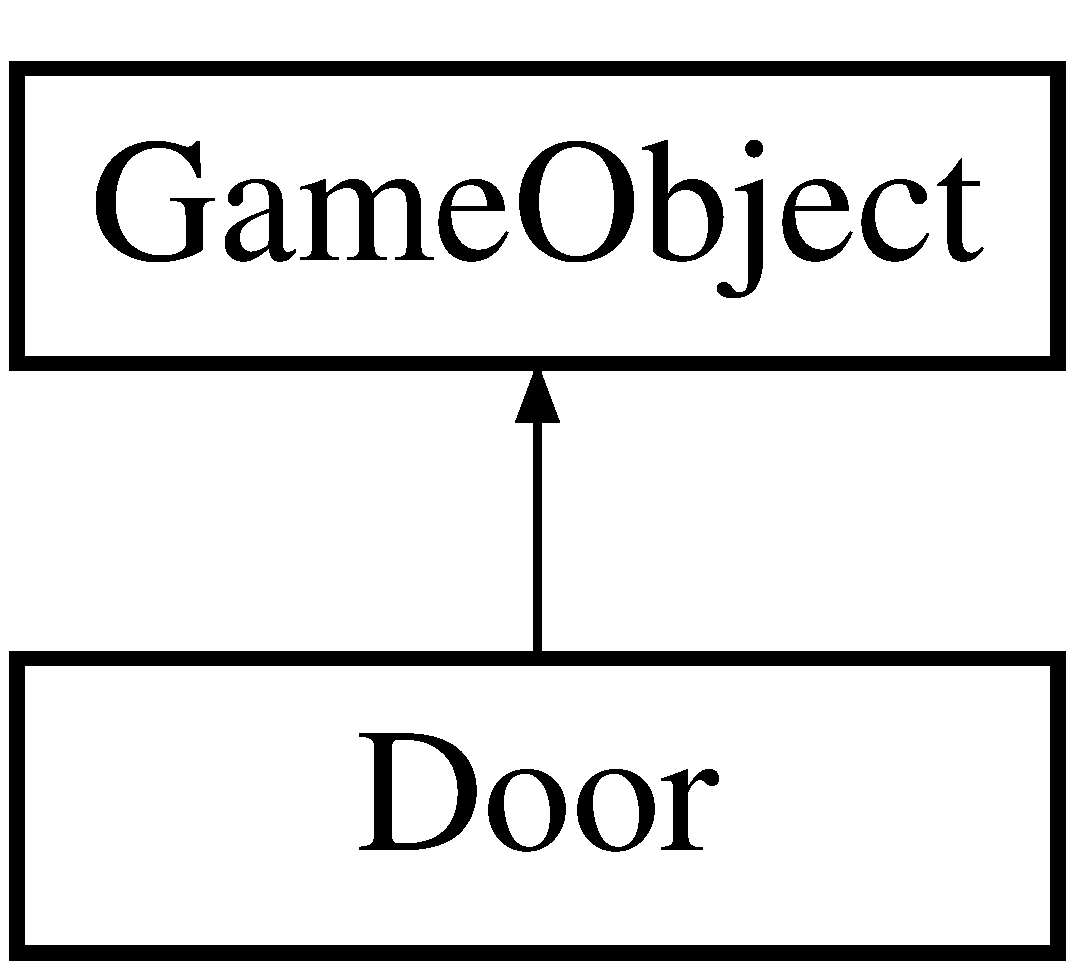
\includegraphics[height=2.000000cm]{classDoor}
\end{center}
\end{figure}
\subsection*{\-Public \-Member \-Functions}
\begin{DoxyCompactItemize}
\item 
\hyperlink{classDoor_a658ddc4507a266a241ad8caa3288c922}{\-Door} (\-Scene\-Manager $\ast$, int)
\item 
virtual \-Game\-State \hyperlink{classDoor_a2e526ecea542d817e04771ed5487bebc}{frame\-Event\-Queued} (\hyperlink{classWayPoint}{\-Way\-Point} $\ast$current\-W\-P, \-Game\-State gs)
\item 
virtual void \hyperlink{classDoor_a6d9a56dd103f3f26b4beaf5682c22187}{init} (\hyperlink{classRoom}{\-Room} $\ast$\hyperlink{classGameObject_a9f63419cc03f2513f757a317a2e37557}{room})
\end{DoxyCompactItemize}
\subsection*{\-Protected \-Member \-Functions}
\begin{DoxyCompactItemize}
\item 
\hyperlink{classDoor_a5191a649ed79b50f886e5c43b473c369}{\-Door} ()
\end{DoxyCompactItemize}
\subsection*{\-Protected \-Attributes}
\begin{DoxyCompactItemize}
\item 
\-Game\-State \hyperlink{classDoor_a3a6559434b958ebf3514348d5065c413}{keys}
\item 
const \-Vector3 \hyperlink{classDoor_a2e00eb490d6c7ea3a37759361fb3d188}{mask}
\end{DoxyCompactItemize}


\subsection{\-Detailed \-Description}
\-Represents a \hyperlink{classDoor}{\-Door} in the demo-\/game. \-A door is a \hyperlink{classGameObject}{\-Game\-Object} and takes care of the appearance, as well as the behaviour of a door. 

\subsection{\-Constructor \& \-Destructor \-Documentation}
\hypertarget{classDoor_a5191a649ed79b50f886e5c43b473c369}{\index{\-Door@{\-Door}!\-Door@{\-Door}}
\index{\-Door@{\-Door}!Door@{\-Door}}
\subsubsection[{\-Door}]{\setlength{\rightskip}{0pt plus 5cm}{\bf \-Door\-::\-Door} (
\begin{DoxyParamCaption}
{}
\end{DoxyParamCaption}
)\hspace{0.3cm}{\ttfamily  \mbox{[}protected\mbox{]}}}}\label{classDoor_a5191a649ed79b50f886e5c43b473c369}
\-Default constructor may not be used outside class scope. \hypertarget{classDoor_a658ddc4507a266a241ad8caa3288c922}{\index{\-Door@{\-Door}!\-Door@{\-Door}}
\index{\-Door@{\-Door}!Door@{\-Door}}
\subsubsection[{\-Door}]{\setlength{\rightskip}{0pt plus 5cm}{\bf \-Door\-::\-Door} (
\begin{DoxyParamCaption}
\item[{\-Scene\-Manager $\ast$}]{, }
\item[{int}]{}
\end{DoxyParamCaption}
)}}\label{classDoor_a658ddc4507a266a241ad8caa3288c922}
\-Constructor\-: initialized the elements for appearance and some game parameters. \-Takes the scene manager (to set up the scene node and entities) and the number of keys that are placed in the game. 

\subsection{\-Member \-Function \-Documentation}
\hypertarget{classDoor_a2e526ecea542d817e04771ed5487bebc}{\index{\-Door@{\-Door}!frame\-Event\-Queued@{frame\-Event\-Queued}}
\index{frame\-Event\-Queued@{frame\-Event\-Queued}!Door@{\-Door}}
\subsubsection[{frame\-Event\-Queued}]{\setlength{\rightskip}{0pt plus 5cm}virtual \-Game\-State {\bf \-Door\-::frame\-Event\-Queued} (
\begin{DoxyParamCaption}
\item[{{\bf \-Way\-Point} $\ast$}]{current\-W\-P, }
\item[{\-Game\-State}]{gs}
\end{DoxyParamCaption}
)\hspace{0.3cm}{\ttfamily  \mbox{[}virtual\mbox{]}}}}\label{classDoor_a2e526ecea542d817e04771ed5487bebc}
\-If the game is in the door event \-Game\-State and the robot reached the trigger. \-Make the room accessible and the door disappear. 

\-Reimplemented from \hyperlink{classGameObject_aa643df342c50df77f053eee2c703c619}{\-Game\-Object}.

\hypertarget{classDoor_a6d9a56dd103f3f26b4beaf5682c22187}{\index{\-Door@{\-Door}!init@{init}}
\index{init@{init}!Door@{\-Door}}
\subsubsection[{init}]{\setlength{\rightskip}{0pt plus 5cm}virtual void {\bf \-Door\-::init} (
\begin{DoxyParamCaption}
\item[{{\bf \-Room} $\ast$}]{room}
\end{DoxyParamCaption}
)\hspace{0.3cm}{\ttfamily  \mbox{[}virtual\mbox{]}}}}\label{classDoor_a6d9a56dd103f3f26b4beaf5682c22187}
(\-Re)\-Initialize the door. \-Place it according to the given room specifications, lock the room and make the virtual door visible again. 

\-Reimplemented from \hyperlink{classGameObject_ac3ab6708ce47b4ef8fd35d8bb43149dc}{\-Game\-Object}.



\subsection{\-Member \-Data \-Documentation}
\hypertarget{classDoor_a3a6559434b958ebf3514348d5065c413}{\index{\-Door@{\-Door}!keys@{keys}}
\index{keys@{keys}!Door@{\-Door}}
\subsubsection[{keys}]{\setlength{\rightskip}{0pt plus 5cm}\-Game\-State {\bf \-Door\-::keys}\hspace{0.3cm}{\ttfamily  \mbox{[}protected\mbox{]}}}}\label{classDoor_a3a6559434b958ebf3514348d5065c413}
\-Specifies in which \-Game\-State the \hyperlink{classDoor}{\-Door} event (to open/disappear) can be triggered. \hypertarget{classDoor_a2e00eb490d6c7ea3a37759361fb3d188}{\index{\-Door@{\-Door}!mask@{mask}}
\index{mask@{mask}!Door@{\-Door}}
\subsubsection[{mask}]{\setlength{\rightskip}{0pt plus 5cm}const \-Vector3 {\bf \-Door\-::mask}\hspace{0.3cm}{\ttfamily  \mbox{[}protected\mbox{]}}}}\label{classDoor_a2e00eb490d6c7ea3a37759361fb3d188}
\-For internal calculation of the door position. 

\-The documentation for this class was generated from the following file\-:\begin{DoxyCompactItemize}
\item 
roculus/include/\-Door.\-h\end{DoxyCompactItemize}

\hypertarget{classGame}{\section{\-Game \-Class \-Reference}
\label{classGame}\index{\-Game@{\-Game}}
}


\-Singleton pattern class to manage the demo-\/game. \-This class manages the demo-\/game and is responsible for all related objects, their (repeatable) initialization and the game process.  




{\ttfamily \#include $<$\-Game.\-h$>$}

\subsection*{\-Public \-Member \-Functions}
\begin{DoxyCompactItemize}
\item 
void \hyperlink{classGame_a2f27f1c291c93f6d7f92e83d887f829f}{init} (\-Scene\-Manager $\ast$)
\item 
\hyperlink{classWayPoint}{\-Way\-Point} $\ast$ \hyperlink{classGame_a866d4f9558c0db8b9df1a86ae8300858}{get\-W\-P\-By\-Id} (int)
\item 
\hyperlink{classWayPoint}{\-Way\-Point} $\ast$ \hyperlink{classGame_aa364e9488c80216844c77ce81b2495a8}{get\-W\-P\-By\-Name} (const \-String \&)
\item 
std\-::string \hyperlink{classGame_af74c96ac1d39ce6f1ca9874c8cef4444}{get\-Init\-W\-P} ()
\item 
\-String \hyperlink{classGame_a8c026e73dbeeb6972f54c3d21a39b89e}{highlight\-Closest\-W\-P} (const \-Vector3 \&)
\item 
\-String \hyperlink{classGame_a62853a0ff9af086067da2dc102850cbb}{get\-State} ()
\item 
void \hyperlink{classGame_a7c39e1c575ef58a513f32fe1a7f42c52}{place\-Persistent\-Marker} (const \-String \&)
\item 
void \hyperlink{classGame_ae954c7759cc186cdf83bd6cc3cfa8419}{print} ()
\item 
void \hyperlink{classGame_ab136a509fabb87b2a0d1fda33d11a457}{start\-Game\-Session} ()
\item 
\-Game\-State \hyperlink{classGame_ae2e9b7906d1484b598edc707b1bd45dd}{frame\-Event\-Queued} (int)
\item 
bool \hyperlink{classGame_a84a979ffa2ce4f8b0df1951a9ce76ecb}{is\-Running} ()
\end{DoxyCompactItemize}
\subsection*{\-Static \-Public \-Member \-Functions}
\begin{DoxyCompactItemize}
\item 
static \hyperlink{classGame}{\-Game} \& \hyperlink{classGame_ab5b377b52d78849aed162538121a20a0}{get\-Instance} ()
\end{DoxyCompactItemize}
\subsection*{\-Protected \-Member \-Functions}
\begin{DoxyCompactItemize}
\item 
\hyperlink{classGame_ad59df6562a58a614fda24622d3715b65}{\-Game} ()
\item 
\hyperlink{classGame_ae3d112ca6e0e55150d2fdbc704474530}{$\sim$\-Game} ()
\item 
\hyperlink{classGame_aa79443880de5f26387c2a1c70c8c1aae}{\-Game} (const \hyperlink{classGame}{\-Game} \&)
\item 
\hyperlink{classGame}{\-Game} \& \hyperlink{classGame_a3face37327a3fcbbdb96494d58d85c48}{operator=} (const \hyperlink{classGame}{\-Game} \&)
\item 
\hyperlink{classRoom}{\-Room} $\ast$ \hyperlink{classGame_aa9c0d063672042d5751fb4c904b6a5b3}{get\-Rnd\-Room} (std\-::set$<$ int $>$ \&room\-N\-Rs)
\end{DoxyCompactItemize}
\subsection*{\-Protected \-Attributes}
\begin{DoxyCompactItemize}
\item 
bool \hyperlink{classGame_aea14eeeea7d21e4ec2353957275aa8d9}{initiated}
\item 
\-Scene\-Manager $\ast$ \hyperlink{classGame_a5f59202a5d81c57c0f1c8f8c717067ff}{m\-Scene\-Mgr}
\item 
\-Scene\-Node $\ast$ \hyperlink{classGame_a1ea0118411f7ae6315bc8e48dea4d074}{marker}
\item 
\-Scene\-Node $\ast$ \hyperlink{classGame_a01b72d441b419041c80ba13b17ccd1a3}{pers\-Marker}
\item 
std\-::vector$<$ \hyperlink{classWayPoint}{\-Way\-Point} $\ast$ $>$ \hyperlink{classGame_ad8fcb3fbae1a4b604fc243e5e2717909}{way\-Points}
\item 
std\-::vector$<$ \hyperlink{classRoom}{\-Room} $\ast$ $>$ \hyperlink{classGame_a2224f48ac11275212f97d0bfad0aa5d0}{rooms}
\item 
std\-::vector$<$ \hyperlink{classRoom}{\-Room} $\ast$ $>$ \hyperlink{classGame_ae3be567935e24e323adfd4d49d345f95}{corridors}
\item 
std\-::vector$<$ \hyperlink{classGameObject}{\-Game\-Object} $\ast$ $>$ \hyperlink{classGame_a9fbc762ef50edb2804683eaafb3d45f3}{game\-Objects}
\item 
\hyperlink{classWayPoint}{\-Way\-Point} $\ast$ \hyperlink{classGame_ab249da316eee71f550d2cb8962c1525f}{select}
\item 
\hyperlink{classWayPoint}{\-Way\-Point} $\ast$ \hyperlink{classGame_a9f00f5b2803e11c6916f5b473b16af74}{init\-W\-P}
\item 
\-Real \hyperlink{classGame_a2ad28722eec0aea922bb205220a80fe8}{dist\-Min}
\item 
\-Real \hyperlink{classGame_a77c996af0e47853d824e25a20faecb0d}{distance}
\item 
\-Game\-State \hyperlink{classGame_ad9fc2a8710ee56916f79314b91112ed0}{state}
\item 
\hyperlink{classDoor}{\-Door} $\ast$ \hyperlink{classGame_af92011162a240ad43f9171329e391942}{door}
\item 
\hyperlink{classTreasure}{\-Treasure} $\ast$ \hyperlink{classGame_ad13ac2228cd02743a92666aa7ecdf5ea}{treasure}
\item 
bool \hyperlink{classGame_a8ca5b9f8a62990e6022de17785beac2c}{running}
\end{DoxyCompactItemize}


\subsection{\-Detailed \-Description}
\-Singleton pattern class to manage the demo-\/game. \-This class manages the demo-\/game and is responsible for all related objects, their (repeatable) initialization and the game process. 

\subsection{\-Constructor \& \-Destructor \-Documentation}
\hypertarget{classGame_ad59df6562a58a614fda24622d3715b65}{\index{\-Game@{\-Game}!\-Game@{\-Game}}
\index{\-Game@{\-Game}!Game@{\-Game}}
\subsubsection[{\-Game}]{\setlength{\rightskip}{0pt plus 5cm}{\bf \-Game\-::\-Game} (
\begin{DoxyParamCaption}
{}
\end{DoxyParamCaption}
)\hspace{0.3cm}{\ttfamily  \mbox{[}inline, protected\mbox{]}}}}\label{classGame_ad59df6562a58a614fda24622d3715b65}
\-Default constructor, not to be used outside class scope. \hypertarget{classGame_ae3d112ca6e0e55150d2fdbc704474530}{\index{\-Game@{\-Game}!$\sim$\-Game@{$\sim$\-Game}}
\index{$\sim$\-Game@{$\sim$\-Game}!Game@{\-Game}}
\subsubsection[{$\sim$\-Game}]{\setlength{\rightskip}{0pt plus 5cm}{\bf \-Game\-::$\sim$\-Game} (
\begin{DoxyParamCaption}
{}
\end{DoxyParamCaption}
)\hspace{0.3cm}{\ttfamily  \mbox{[}protected\mbox{]}}}}\label{classGame_ae3d112ca6e0e55150d2fdbc704474530}
\-Default destructor. \hypertarget{classGame_aa79443880de5f26387c2a1c70c8c1aae}{\index{\-Game@{\-Game}!\-Game@{\-Game}}
\index{\-Game@{\-Game}!Game@{\-Game}}
\subsubsection[{\-Game}]{\setlength{\rightskip}{0pt plus 5cm}{\bf \-Game\-::\-Game} (
\begin{DoxyParamCaption}
\item[{const {\bf \-Game} \&}]{}
\end{DoxyParamCaption}
)\hspace{0.3cm}{\ttfamily  \mbox{[}protected\mbox{]}}}}\label{classGame_aa79443880de5f26387c2a1c70c8c1aae}
\-Copy constructor, hidden due to singleton pattern. 

\subsection{\-Member \-Function \-Documentation}
\hypertarget{classGame_ae2e9b7906d1484b598edc707b1bd45dd}{\index{\-Game@{\-Game}!frame\-Event\-Queued@{frame\-Event\-Queued}}
\index{frame\-Event\-Queued@{frame\-Event\-Queued}!Game@{\-Game}}
\subsubsection[{frame\-Event\-Queued}]{\setlength{\rightskip}{0pt plus 5cm}\-Game\-State {\bf \-Game\-::frame\-Event\-Queued} (
\begin{DoxyParamCaption}
\item[{int}]{}
\end{DoxyParamCaption}
)}}\label{classGame_ae2e9b7906d1484b598edc707b1bd45dd}
\-Process the game. \-The \-Game\-State is known internally, the parameter is the current waypoint \-I\-D of the robot. \hypertarget{classGame_af74c96ac1d39ce6f1ca9874c8cef4444}{\index{\-Game@{\-Game}!get\-Init\-W\-P@{get\-Init\-W\-P}}
\index{get\-Init\-W\-P@{get\-Init\-W\-P}!Game@{\-Game}}
\subsubsection[{get\-Init\-W\-P}]{\setlength{\rightskip}{0pt plus 5cm}std\-::string {\bf \-Game\-::get\-Init\-W\-P} (
\begin{DoxyParamCaption}
{}
\end{DoxyParamCaption}
)}}\label{classGame_af74c96ac1d39ce6f1ca9874c8cef4444}
\-Get the waypoint the game shall be started at (robot location). \hypertarget{classGame_ab5b377b52d78849aed162538121a20a0}{\index{\-Game@{\-Game}!get\-Instance@{get\-Instance}}
\index{get\-Instance@{get\-Instance}!Game@{\-Game}}
\subsubsection[{get\-Instance}]{\setlength{\rightskip}{0pt plus 5cm}static {\bf \-Game}\& {\bf \-Game\-::get\-Instance} (
\begin{DoxyParamCaption}
{}
\end{DoxyParamCaption}
)\hspace{0.3cm}{\ttfamily  \mbox{[}static\mbox{]}}}}\label{classGame_ab5b377b52d78849aed162538121a20a0}
\-Get the single instance of the \hyperlink{classGame}{\-Game} class. \hypertarget{classGame_aa9c0d063672042d5751fb4c904b6a5b3}{\index{\-Game@{\-Game}!get\-Rnd\-Room@{get\-Rnd\-Room}}
\index{get\-Rnd\-Room@{get\-Rnd\-Room}!Game@{\-Game}}
\subsubsection[{get\-Rnd\-Room}]{\setlength{\rightskip}{0pt plus 5cm}{\bf \-Room}$\ast$ {\bf \-Game\-::get\-Rnd\-Room} (
\begin{DoxyParamCaption}
\item[{std\-::set$<$ int $>$ \&}]{room\-N\-Rs}
\end{DoxyParamCaption}
)\hspace{0.3cm}{\ttfamily  \mbox{[}protected\mbox{]}}}}\label{classGame_aa9c0d063672042d5751fb4c904b6a5b3}
\-Utility function\-: get a random room from the set of all rooms and erase that room number/index from the set. \hypertarget{classGame_a62853a0ff9af086067da2dc102850cbb}{\index{\-Game@{\-Game}!get\-State@{get\-State}}
\index{get\-State@{get\-State}!Game@{\-Game}}
\subsubsection[{get\-State}]{\setlength{\rightskip}{0pt plus 5cm}\-String {\bf \-Game\-::get\-State} (
\begin{DoxyParamCaption}
{}
\end{DoxyParamCaption}
)}}\label{classGame_a62853a0ff9af086067da2dc102850cbb}
\-Return the \-Game\-State. \hypertarget{classGame_a866d4f9558c0db8b9df1a86ae8300858}{\index{\-Game@{\-Game}!get\-W\-P\-By\-Id@{get\-W\-P\-By\-Id}}
\index{get\-W\-P\-By\-Id@{get\-W\-P\-By\-Id}!Game@{\-Game}}
\subsubsection[{get\-W\-P\-By\-Id}]{\setlength{\rightskip}{0pt plus 5cm}{\bf \-Way\-Point}$\ast$ {\bf \-Game\-::get\-W\-P\-By\-Id} (
\begin{DoxyParamCaption}
\item[{int}]{}
\end{DoxyParamCaption}
)}}\label{classGame_a866d4f9558c0db8b9df1a86ae8300858}
\-Get a waypoint using its \-I\-D as identifier. \hypertarget{classGame_aa364e9488c80216844c77ce81b2495a8}{\index{\-Game@{\-Game}!get\-W\-P\-By\-Name@{get\-W\-P\-By\-Name}}
\index{get\-W\-P\-By\-Name@{get\-W\-P\-By\-Name}!Game@{\-Game}}
\subsubsection[{get\-W\-P\-By\-Name}]{\setlength{\rightskip}{0pt plus 5cm}{\bf \-Way\-Point}$\ast$ {\bf \-Game\-::get\-W\-P\-By\-Name} (
\begin{DoxyParamCaption}
\item[{const \-String \&}]{}
\end{DoxyParamCaption}
)}}\label{classGame_aa364e9488c80216844c77ce81b2495a8}
\-Get a waypoint using its name as identifier. \-String search is not very performant -\/$>$ use with care. (\-Not \-E\-A\-C\-H frame!!!). \hypertarget{classGame_a8c026e73dbeeb6972f54c3d21a39b89e}{\index{\-Game@{\-Game}!highlight\-Closest\-W\-P@{highlight\-Closest\-W\-P}}
\index{highlight\-Closest\-W\-P@{highlight\-Closest\-W\-P}!Game@{\-Game}}
\subsubsection[{highlight\-Closest\-W\-P}]{\setlength{\rightskip}{0pt plus 5cm}\-String {\bf \-Game\-::highlight\-Closest\-W\-P} (
\begin{DoxyParamCaption}
\item[{const \-Vector3 \&}]{}
\end{DoxyParamCaption}
)}}\label{classGame_a8c026e73dbeeb6972f54c3d21a39b89e}
\-Find the closest waypoint and return its name. \hypertarget{classGame_a2f27f1c291c93f6d7f92e83d887f829f}{\index{\-Game@{\-Game}!init@{init}}
\index{init@{init}!Game@{\-Game}}
\subsubsection[{init}]{\setlength{\rightskip}{0pt plus 5cm}void {\bf \-Game\-::init} (
\begin{DoxyParamCaption}
\item[{\-Scene\-Manager $\ast$}]{}
\end{DoxyParamCaption}
)}}\label{classGame_a2f27f1c291c93f6d7f92e83d887f829f}
\-Initialize the \hyperlink{classGame}{\-Game} class. \-Has to be called before the singleton can be used with \hyperlink{classGame_ab5b377b52d78849aed162538121a20a0}{get\-Instance()}. \hypertarget{classGame_a84a979ffa2ce4f8b0df1951a9ce76ecb}{\index{\-Game@{\-Game}!is\-Running@{is\-Running}}
\index{is\-Running@{is\-Running}!Game@{\-Game}}
\subsubsection[{is\-Running}]{\setlength{\rightskip}{0pt plus 5cm}bool {\bf \-Game\-::is\-Running} (
\begin{DoxyParamCaption}
{}
\end{DoxyParamCaption}
)}}\label{classGame_a84a979ffa2ce4f8b0df1951a9ce76ecb}
\-Is the game running? \hypertarget{classGame_a3face37327a3fcbbdb96494d58d85c48}{\index{\-Game@{\-Game}!operator=@{operator=}}
\index{operator=@{operator=}!Game@{\-Game}}
\subsubsection[{operator=}]{\setlength{\rightskip}{0pt plus 5cm}{\bf \-Game}\& \-Game\-::operator= (
\begin{DoxyParamCaption}
\item[{const {\bf \-Game} \&}]{}
\end{DoxyParamCaption}
)\hspace{0.3cm}{\ttfamily  \mbox{[}protected\mbox{]}}}}\label{classGame_a3face37327a3fcbbdb96494d58d85c48}
\-Copy operator, hidden due to singleton pattern. \hypertarget{classGame_a7c39e1c575ef58a513f32fe1a7f42c52}{\index{\-Game@{\-Game}!place\-Persistent\-Marker@{place\-Persistent\-Marker}}
\index{place\-Persistent\-Marker@{place\-Persistent\-Marker}!Game@{\-Game}}
\subsubsection[{place\-Persistent\-Marker}]{\setlength{\rightskip}{0pt plus 5cm}void {\bf \-Game\-::place\-Persistent\-Marker} (
\begin{DoxyParamCaption}
\item[{const \-String \&}]{}
\end{DoxyParamCaption}
)}}\label{classGame_a7c39e1c575ef58a513f32fe1a7f42c52}
\-Place the persistent marker (for the navigation target) on the waypoint specified by name. \hypertarget{classGame_ae954c7759cc186cdf83bd6cc3cfa8419}{\index{\-Game@{\-Game}!print@{print}}
\index{print@{print}!Game@{\-Game}}
\subsubsection[{print}]{\setlength{\rightskip}{0pt plus 5cm}void {\bf \-Game\-::print} (
\begin{DoxyParamCaption}
{}
\end{DoxyParamCaption}
)}}\label{classGame_ae954c7759cc186cdf83bd6cc3cfa8419}
\-Print the configuration of the game (waypoints, corridors, rooms) on the console. \-Useful for debugging. \hypertarget{classGame_ab136a509fabb87b2a0d1fda33d11a457}{\index{\-Game@{\-Game}!start\-Game\-Session@{start\-Game\-Session}}
\index{start\-Game\-Session@{start\-Game\-Session}!Game@{\-Game}}
\subsubsection[{start\-Game\-Session}]{\setlength{\rightskip}{0pt plus 5cm}void {\bf \-Game\-::start\-Game\-Session} (
\begin{DoxyParamCaption}
{}
\end{DoxyParamCaption}
)}}\label{classGame_ab136a509fabb87b2a0d1fda33d11a457}
\-Start a new game (reinitialize). 

\subsection{\-Member \-Data \-Documentation}
\hypertarget{classGame_ae3be567935e24e323adfd4d49d345f95}{\index{\-Game@{\-Game}!corridors@{corridors}}
\index{corridors@{corridors}!Game@{\-Game}}
\subsubsection[{corridors}]{\setlength{\rightskip}{0pt plus 5cm}std\-::vector$<${\bf \-Room}$\ast$$>$ {\bf \-Game\-::corridors}\hspace{0.3cm}{\ttfamily  \mbox{[}protected\mbox{]}}}}\label{classGame_ae3be567935e24e323adfd4d49d345f95}
\-Vector of all corridors. \hypertarget{classGame_a77c996af0e47853d824e25a20faecb0d}{\index{\-Game@{\-Game}!distance@{distance}}
\index{distance@{distance}!Game@{\-Game}}
\subsubsection[{distance}]{\setlength{\rightskip}{0pt plus 5cm}\-Real {\bf \-Game\-::distance}\hspace{0.3cm}{\ttfamily  \mbox{[}protected\mbox{]}}}}\label{classGame_a77c996af0e47853d824e25a20faecb0d}
\-Internal calculus, global to avoid continuous memory alloc.\-: distance for the current iteration of the sorting algorithm. \hypertarget{classGame_a2ad28722eec0aea922bb205220a80fe8}{\index{\-Game@{\-Game}!dist\-Min@{dist\-Min}}
\index{dist\-Min@{dist\-Min}!Game@{\-Game}}
\subsubsection[{dist\-Min}]{\setlength{\rightskip}{0pt plus 5cm}\-Real {\bf \-Game\-::dist\-Min}\hspace{0.3cm}{\ttfamily  \mbox{[}protected\mbox{]}}}}\label{classGame_a2ad28722eec0aea922bb205220a80fe8}
\-Internal calculus, global to avoid continuous memory alloc.\-: current found min. distance in the sorting algorithm. \hypertarget{classGame_af92011162a240ad43f9171329e391942}{\index{\-Game@{\-Game}!door@{door}}
\index{door@{door}!Game@{\-Game}}
\subsubsection[{door}]{\setlength{\rightskip}{0pt plus 5cm}{\bf \-Door}$\ast$ {\bf \-Game\-::door}\hspace{0.3cm}{\ttfamily  \mbox{[}protected\mbox{]}}}}\label{classGame_af92011162a240ad43f9171329e391942}
\-The door in the game (there is just one). \hypertarget{classGame_a9fbc762ef50edb2804683eaafb3d45f3}{\index{\-Game@{\-Game}!game\-Objects@{game\-Objects}}
\index{game\-Objects@{game\-Objects}!Game@{\-Game}}
\subsubsection[{game\-Objects}]{\setlength{\rightskip}{0pt plus 5cm}std\-::vector$<${\bf \-Game\-Object}$\ast$$>$ {\bf \-Game\-::game\-Objects}\hspace{0.3cm}{\ttfamily  \mbox{[}protected\mbox{]}}}}\label{classGame_a9fbc762ef50edb2804683eaafb3d45f3}
\-Vector of all \-Game\-Objects. \hypertarget{classGame_aea14eeeea7d21e4ec2353957275aa8d9}{\index{\-Game@{\-Game}!initiated@{initiated}}
\index{initiated@{initiated}!Game@{\-Game}}
\subsubsection[{initiated}]{\setlength{\rightskip}{0pt plus 5cm}bool {\bf \-Game\-::initiated}\hspace{0.3cm}{\ttfamily  \mbox{[}protected\mbox{]}}}}\label{classGame_aea14eeeea7d21e4ec2353957275aa8d9}
\-Marks if the game was successfully initiated for the first time. \hypertarget{classGame_a9f00f5b2803e11c6916f5b473b16af74}{\index{\-Game@{\-Game}!init\-W\-P@{init\-W\-P}}
\index{init\-W\-P@{init\-W\-P}!Game@{\-Game}}
\subsubsection[{init\-W\-P}]{\setlength{\rightskip}{0pt plus 5cm}{\bf \-Way\-Point}$\ast$ {\bf \-Game\-::init\-W\-P}\hspace{0.3cm}{\ttfamily  \mbox{[}protected\mbox{]}}}}\label{classGame_a9f00f5b2803e11c6916f5b473b16af74}
\-Currently not in use, but generally the waypoint the robot should navigate to, if the game is restarted. \-The code for this should be commented-\/in in \hyperlink{classBaseApplication}{\-Base\-Application}. \hypertarget{classGame_a1ea0118411f7ae6315bc8e48dea4d074}{\index{\-Game@{\-Game}!marker@{marker}}
\index{marker@{marker}!Game@{\-Game}}
\subsubsection[{marker}]{\setlength{\rightskip}{0pt plus 5cm}\-Scene\-Node$\ast$ {\bf \-Game\-::marker}\hspace{0.3cm}{\ttfamily  \mbox{[}protected\mbox{]}}}}\label{classGame_a1ea0118411f7ae6315bc8e48dea4d074}
\-The waypoint marker (green flagg) that will jump between possible navigation targets. \hypertarget{classGame_a5f59202a5d81c57c0f1c8f8c717067ff}{\index{\-Game@{\-Game}!m\-Scene\-Mgr@{m\-Scene\-Mgr}}
\index{m\-Scene\-Mgr@{m\-Scene\-Mgr}!Game@{\-Game}}
\subsubsection[{m\-Scene\-Mgr}]{\setlength{\rightskip}{0pt plus 5cm}\-Scene\-Manager$\ast$ {\bf \-Game\-::m\-Scene\-Mgr}\hspace{0.3cm}{\ttfamily  \mbox{[}protected\mbox{]}}}}\label{classGame_a5f59202a5d81c57c0f1c8f8c717067ff}
\-The scene manager (used for object creation). \hypertarget{classGame_a01b72d441b419041c80ba13b17ccd1a3}{\index{\-Game@{\-Game}!pers\-Marker@{pers\-Marker}}
\index{pers\-Marker@{pers\-Marker}!Game@{\-Game}}
\subsubsection[{pers\-Marker}]{\setlength{\rightskip}{0pt plus 5cm}\-Scene\-Node $\ast$ {\bf \-Game\-::pers\-Marker}\hspace{0.3cm}{\ttfamily  \mbox{[}protected\mbox{]}}}}\label{classGame_a01b72d441b419041c80ba13b17ccd1a3}
\-The waypoint marker (red flagg) that will stay on the current navigation target. \hypertarget{classGame_a2224f48ac11275212f97d0bfad0aa5d0}{\index{\-Game@{\-Game}!rooms@{rooms}}
\index{rooms@{rooms}!Game@{\-Game}}
\subsubsection[{rooms}]{\setlength{\rightskip}{0pt plus 5cm}std\-::vector$<${\bf \-Room}$\ast$$>$ {\bf \-Game\-::rooms}\hspace{0.3cm}{\ttfamily  \mbox{[}protected\mbox{]}}}}\label{classGame_a2224f48ac11275212f97d0bfad0aa5d0}
\-Vector of all rooms. \hypertarget{classGame_a8ca5b9f8a62990e6022de17785beac2c}{\index{\-Game@{\-Game}!running@{running}}
\index{running@{running}!Game@{\-Game}}
\subsubsection[{running}]{\setlength{\rightskip}{0pt plus 5cm}bool {\bf \-Game\-::running}\hspace{0.3cm}{\ttfamily  \mbox{[}protected\mbox{]}}}}\label{classGame_a8ca5b9f8a62990e6022de17785beac2c}
\-Is the game initialized and started? \hypertarget{classGame_ab249da316eee71f550d2cb8962c1525f}{\index{\-Game@{\-Game}!select@{select}}
\index{select@{select}!Game@{\-Game}}
\subsubsection[{select}]{\setlength{\rightskip}{0pt plus 5cm}{\bf \-Way\-Point}$\ast$ {\bf \-Game\-::select}\hspace{0.3cm}{\ttfamily  \mbox{[}protected\mbox{]}}}}\label{classGame_ab249da316eee71f550d2cb8962c1525f}
\-Waypoint to which the cursor is closest (with some maximum distance threshold). \hypertarget{classGame_ad9fc2a8710ee56916f79314b91112ed0}{\index{\-Game@{\-Game}!state@{state}}
\index{state@{state}!Game@{\-Game}}
\subsubsection[{state}]{\setlength{\rightskip}{0pt plus 5cm}\-Game\-State {\bf \-Game\-::state}\hspace{0.3cm}{\ttfamily  \mbox{[}protected\mbox{]}}}}\label{classGame_ad9fc2a8710ee56916f79314b91112ed0}
\-The current state of the game. \hypertarget{classGame_ad13ac2228cd02743a92666aa7ecdf5ea}{\index{\-Game@{\-Game}!treasure@{treasure}}
\index{treasure@{treasure}!Game@{\-Game}}
\subsubsection[{treasure}]{\setlength{\rightskip}{0pt plus 5cm}{\bf \-Treasure}$\ast$ {\bf \-Game\-::treasure}\hspace{0.3cm}{\ttfamily  \mbox{[}protected\mbox{]}}}}\label{classGame_ad13ac2228cd02743a92666aa7ecdf5ea}
\-The treasure in the game (there is just one). \hypertarget{classGame_ad8fcb3fbae1a4b604fc243e5e2717909}{\index{\-Game@{\-Game}!way\-Points@{way\-Points}}
\index{way\-Points@{way\-Points}!Game@{\-Game}}
\subsubsection[{way\-Points}]{\setlength{\rightskip}{0pt plus 5cm}std\-::vector$<${\bf \-Way\-Point}$\ast$$>$ {\bf \-Game\-::way\-Points}\hspace{0.3cm}{\ttfamily  \mbox{[}protected\mbox{]}}}}\label{classGame_ad8fcb3fbae1a4b604fc243e5e2717909}
\-Vector of all waypoints. 

\-The documentation for this class was generated from the following file\-:\begin{DoxyCompactItemize}
\item 
roculus/include/\-Game.\-h\end{DoxyCompactItemize}

\hypertarget{classGameCFGParser}{\section{\-Game\-C\-F\-G\-Parser \-Class \-Reference}
\label{classGameCFGParser}\index{\-Game\-C\-F\-G\-Parser@{\-Game\-C\-F\-G\-Parser}}
}


\-Parses the 'game.\-cfg' file. \-This class provides an easy-\/to-\/use parser for the config file of a game. \-Note that the filename is hardcoded in the constructor.  




{\ttfamily \#include $<$\-Game\-C\-F\-G\-Parser.\-h$>$}

\subsection*{\-Public \-Member \-Functions}
\begin{DoxyCompactItemize}
\item 
std\-::string \hyperlink{classGameCFGParser_ad703ab9f55a3542232f90f6b87cd85e5}{get\-Init\-Node} ()
\item 
int \hyperlink{classGameCFGParser_a48546c5931ccc40303713cdbbc3362f7}{get\-Nr\-Keys} ()
\item 
int \hyperlink{classGameCFGParser_ac7001b9a73ab8d89870d4a01d3fcb3e9}{get\-Nr\-Rooms} ()
\item 
int \hyperlink{classGameCFGParser_af35e4757b4cb39753b3a3779252ef61f}{get\-Nr\-Corridors} ()
\item 
int \hyperlink{classGameCFGParser_a4762e0fc122db2360a01d92ccf66a290}{get\-Nr\-Way\-Points} ()
\item 
int \hyperlink{classGameCFGParser_af4e55769fb6c312e1946320f5871d137}{get\-Door} (const std\-::string \&)
\item 
int \hyperlink{classGameCFGParser_a331c9e8f80f4e9db2712062e8526ea0d}{get\-Door\-Evt} (const std\-::string \&)
\item 
std\-::vector$<$ int $>$ \hyperlink{classGameCFGParser_a6ebc74939d28da7cfd68018202aba3f4}{get\-W\-Ps2\-Use} (const std\-::string \&)
\item 
std\-::vector$<$ int $>$ \hyperlink{classGameCFGParser_a88232d196c405ce5736749db1f200981}{get\-W\-Ps} (const std\-::string \&)
\item 
std\-::string \hyperlink{classGameCFGParser_adb5f04b377373467e3568c546e1b0eb2}{get\-Value\-As\-String} (const std\-::string \&)
\item 
bool \hyperlink{classGameCFGParser_ab283cea504bf1db9d35a89e95b285402}{get\-Key\-Exists} (const std\-::string \&)
\end{DoxyCompactItemize}
\subsection*{\-Static \-Public \-Member \-Functions}
\begin{DoxyCompactItemize}
\item 
static \hyperlink{classGameCFGParser}{\-Game\-C\-F\-G\-Parser} \& \hyperlink{classGameCFGParser_a5e16899911e9978520f2b3899f05ca36}{get\-Instance} ()
\end{DoxyCompactItemize}
\subsection*{\-Protected \-Member \-Functions}
\begin{DoxyCompactItemize}
\item 
\hyperlink{classGameCFGParser_ad746b796abbe8e061e3da92e08d3dab7}{\-Game\-C\-F\-G\-Parser} ()
\item 
\hyperlink{classGameCFGParser_a2abbb5569224df6be70644311d524433}{$\sim$\-Game\-C\-F\-G\-Parser} ()
\item 
\hyperlink{classGameCFGParser_a50298175551786f51749010622390163}{\-Game\-C\-F\-G\-Parser} (const \hyperlink{classGameCFGParser}{\-Game\-C\-F\-G\-Parser} \&)
\item 
\hyperlink{classGameCFGParser}{\-Game\-C\-F\-G\-Parser} \& \hyperlink{classGameCFGParser_a8f95dc8cadfc64f785fa929d63339220}{operator=} (const \hyperlink{classGameCFGParser}{\-Game\-C\-F\-G\-Parser} \&)
\end{DoxyCompactItemize}
\subsection*{\-Protected \-Attributes}
\begin{DoxyCompactItemize}
\item 
\-Ogre\-::\-Config\-File \hyperlink{classGameCFGParser_a959aad3003435f1deef6f92ca7902316}{game\-\_\-cfg}
\item 
std\-::map$<$ std\-::string, \*
std\-::string $>$ \hyperlink{classGameCFGParser_a4c61cec38365caa5ed4650eff682ecd9}{m\-\_\-\-Config}
\item 
int \hyperlink{classGameCFGParser_a42c185380b0fb82948ef24fcdbcf1f0f}{cnt\-Corridors}
\item 
int \hyperlink{classGameCFGParser_a026f91734a398714a8e8fae1fa3a4f7f}{cnt\-Rooms}
\end{DoxyCompactItemize}


\subsection{\-Detailed \-Description}
\-Parses the 'game.\-cfg' file. \-This class provides an easy-\/to-\/use parser for the config file of a game. \-Note that the filename is hardcoded in the constructor. 

\subsection{\-Constructor \& \-Destructor \-Documentation}
\hypertarget{classGameCFGParser_ad746b796abbe8e061e3da92e08d3dab7}{\index{\-Game\-C\-F\-G\-Parser@{\-Game\-C\-F\-G\-Parser}!\-Game\-C\-F\-G\-Parser@{\-Game\-C\-F\-G\-Parser}}
\index{\-Game\-C\-F\-G\-Parser@{\-Game\-C\-F\-G\-Parser}!GameCFGParser@{\-Game\-C\-F\-G\-Parser}}
\subsubsection[{\-Game\-C\-F\-G\-Parser}]{\setlength{\rightskip}{0pt plus 5cm}{\bf \-Game\-C\-F\-G\-Parser\-::\-Game\-C\-F\-G\-Parser} (
\begin{DoxyParamCaption}
{}
\end{DoxyParamCaption}
)\hspace{0.3cm}{\ttfamily  \mbox{[}protected\mbox{]}}}}\label{classGameCFGParser_ad746b796abbe8e061e3da92e08d3dab7}
\-Default constructor. \-Hidden due to \-Singleton pattern. \hypertarget{classGameCFGParser_a2abbb5569224df6be70644311d524433}{\index{\-Game\-C\-F\-G\-Parser@{\-Game\-C\-F\-G\-Parser}!$\sim$\-Game\-C\-F\-G\-Parser@{$\sim$\-Game\-C\-F\-G\-Parser}}
\index{$\sim$\-Game\-C\-F\-G\-Parser@{$\sim$\-Game\-C\-F\-G\-Parser}!GameCFGParser@{\-Game\-C\-F\-G\-Parser}}
\subsubsection[{$\sim$\-Game\-C\-F\-G\-Parser}]{\setlength{\rightskip}{0pt plus 5cm}{\bf \-Game\-C\-F\-G\-Parser\-::$\sim$\-Game\-C\-F\-G\-Parser} (
\begin{DoxyParamCaption}
{}
\end{DoxyParamCaption}
)\hspace{0.3cm}{\ttfamily  \mbox{[}protected\mbox{]}}}}\label{classGameCFGParser_a2abbb5569224df6be70644311d524433}
\-Default destructor. \-Hidden due to \-Singleton pattern. \hypertarget{classGameCFGParser_a50298175551786f51749010622390163}{\index{\-Game\-C\-F\-G\-Parser@{\-Game\-C\-F\-G\-Parser}!\-Game\-C\-F\-G\-Parser@{\-Game\-C\-F\-G\-Parser}}
\index{\-Game\-C\-F\-G\-Parser@{\-Game\-C\-F\-G\-Parser}!GameCFGParser@{\-Game\-C\-F\-G\-Parser}}
\subsubsection[{\-Game\-C\-F\-G\-Parser}]{\setlength{\rightskip}{0pt plus 5cm}{\bf \-Game\-C\-F\-G\-Parser\-::\-Game\-C\-F\-G\-Parser} (
\begin{DoxyParamCaption}
\item[{const {\bf \-Game\-C\-F\-G\-Parser} \&}]{}
\end{DoxyParamCaption}
)\hspace{0.3cm}{\ttfamily  \mbox{[}protected\mbox{]}}}}\label{classGameCFGParser_a50298175551786f51749010622390163}
\-Copy constructor. \-Hidden due to \-Singleton pattern. 

\subsection{\-Member \-Function \-Documentation}
\hypertarget{classGameCFGParser_af4e55769fb6c312e1946320f5871d137}{\index{\-Game\-C\-F\-G\-Parser@{\-Game\-C\-F\-G\-Parser}!get\-Door@{get\-Door}}
\index{get\-Door@{get\-Door}!GameCFGParser@{\-Game\-C\-F\-G\-Parser}}
\subsubsection[{get\-Door}]{\setlength{\rightskip}{0pt plus 5cm}int {\bf \-Game\-C\-F\-G\-Parser\-::get\-Door} (
\begin{DoxyParamCaption}
\item[{const std\-::string \&}]{}
\end{DoxyParamCaption}
)}}\label{classGameCFGParser_af4e55769fb6c312e1946320f5871d137}
\-Returns the index of the 'door' waypoint in the specified room. \hypertarget{classGameCFGParser_a331c9e8f80f4e9db2712062e8526ea0d}{\index{\-Game\-C\-F\-G\-Parser@{\-Game\-C\-F\-G\-Parser}!get\-Door\-Evt@{get\-Door\-Evt}}
\index{get\-Door\-Evt@{get\-Door\-Evt}!GameCFGParser@{\-Game\-C\-F\-G\-Parser}}
\subsubsection[{get\-Door\-Evt}]{\setlength{\rightskip}{0pt plus 5cm}int {\bf \-Game\-C\-F\-G\-Parser\-::get\-Door\-Evt} (
\begin{DoxyParamCaption}
\item[{const std\-::string \&}]{}
\end{DoxyParamCaption}
)}}\label{classGameCFGParser_a331c9e8f80f4e9db2712062e8526ea0d}
\-Returns the index of the 'door event' waypoint in the specified room. \hypertarget{classGameCFGParser_ad703ab9f55a3542232f90f6b87cd85e5}{\index{\-Game\-C\-F\-G\-Parser@{\-Game\-C\-F\-G\-Parser}!get\-Init\-Node@{get\-Init\-Node}}
\index{get\-Init\-Node@{get\-Init\-Node}!GameCFGParser@{\-Game\-C\-F\-G\-Parser}}
\subsubsection[{get\-Init\-Node}]{\setlength{\rightskip}{0pt plus 5cm}std\-::string {\bf \-Game\-C\-F\-G\-Parser\-::get\-Init\-Node} (
\begin{DoxyParamCaption}
{}
\end{DoxyParamCaption}
)}}\label{classGameCFGParser_ad703ab9f55a3542232f90f6b87cd85e5}
\-Returns the node at which the game should be started (with the robot on it). \hypertarget{classGameCFGParser_a5e16899911e9978520f2b3899f05ca36}{\index{\-Game\-C\-F\-G\-Parser@{\-Game\-C\-F\-G\-Parser}!get\-Instance@{get\-Instance}}
\index{get\-Instance@{get\-Instance}!GameCFGParser@{\-Game\-C\-F\-G\-Parser}}
\subsubsection[{get\-Instance}]{\setlength{\rightskip}{0pt plus 5cm}static {\bf \-Game\-C\-F\-G\-Parser}\& {\bf \-Game\-C\-F\-G\-Parser\-::get\-Instance} (
\begin{DoxyParamCaption}
{}
\end{DoxyParamCaption}
)\hspace{0.3cm}{\ttfamily  \mbox{[}static\mbox{]}}}}\label{classGameCFGParser_a5e16899911e9978520f2b3899f05ca36}
\-Get the (single) instance of this class. \hypertarget{classGameCFGParser_ab283cea504bf1db9d35a89e95b285402}{\index{\-Game\-C\-F\-G\-Parser@{\-Game\-C\-F\-G\-Parser}!get\-Key\-Exists@{get\-Key\-Exists}}
\index{get\-Key\-Exists@{get\-Key\-Exists}!GameCFGParser@{\-Game\-C\-F\-G\-Parser}}
\subsubsection[{get\-Key\-Exists}]{\setlength{\rightskip}{0pt plus 5cm}bool {\bf \-Game\-C\-F\-G\-Parser\-::get\-Key\-Exists} (
\begin{DoxyParamCaption}
\item[{const std\-::string \&}]{}
\end{DoxyParamCaption}
)}}\label{classGameCFGParser_ab283cea504bf1db9d35a89e95b285402}
\-Checks whether the specified key exists (return true), or not (false). \hypertarget{classGameCFGParser_af35e4757b4cb39753b3a3779252ef61f}{\index{\-Game\-C\-F\-G\-Parser@{\-Game\-C\-F\-G\-Parser}!get\-Nr\-Corridors@{get\-Nr\-Corridors}}
\index{get\-Nr\-Corridors@{get\-Nr\-Corridors}!GameCFGParser@{\-Game\-C\-F\-G\-Parser}}
\subsubsection[{get\-Nr\-Corridors}]{\setlength{\rightskip}{0pt plus 5cm}int {\bf \-Game\-C\-F\-G\-Parser\-::get\-Nr\-Corridors} (
\begin{DoxyParamCaption}
{}
\end{DoxyParamCaption}
)}}\label{classGameCFGParser_af35e4757b4cb39753b3a3779252ef61f}
\-Returns the number of corridors in the game. \hypertarget{classGameCFGParser_a48546c5931ccc40303713cdbbc3362f7}{\index{\-Game\-C\-F\-G\-Parser@{\-Game\-C\-F\-G\-Parser}!get\-Nr\-Keys@{get\-Nr\-Keys}}
\index{get\-Nr\-Keys@{get\-Nr\-Keys}!GameCFGParser@{\-Game\-C\-F\-G\-Parser}}
\subsubsection[{get\-Nr\-Keys}]{\setlength{\rightskip}{0pt plus 5cm}int {\bf \-Game\-C\-F\-G\-Parser\-::get\-Nr\-Keys} (
\begin{DoxyParamCaption}
{}
\end{DoxyParamCaption}
)}}\label{classGameCFGParser_a48546c5931ccc40303713cdbbc3362f7}
\-Returns the number of keys that are placed in the game. \hypertarget{classGameCFGParser_ac7001b9a73ab8d89870d4a01d3fcb3e9}{\index{\-Game\-C\-F\-G\-Parser@{\-Game\-C\-F\-G\-Parser}!get\-Nr\-Rooms@{get\-Nr\-Rooms}}
\index{get\-Nr\-Rooms@{get\-Nr\-Rooms}!GameCFGParser@{\-Game\-C\-F\-G\-Parser}}
\subsubsection[{get\-Nr\-Rooms}]{\setlength{\rightskip}{0pt plus 5cm}int {\bf \-Game\-C\-F\-G\-Parser\-::get\-Nr\-Rooms} (
\begin{DoxyParamCaption}
{}
\end{DoxyParamCaption}
)}}\label{classGameCFGParser_ac7001b9a73ab8d89870d4a01d3fcb3e9}
\-Retruns the number of rooms in the game. \hypertarget{classGameCFGParser_a4762e0fc122db2360a01d92ccf66a290}{\index{\-Game\-C\-F\-G\-Parser@{\-Game\-C\-F\-G\-Parser}!get\-Nr\-Way\-Points@{get\-Nr\-Way\-Points}}
\index{get\-Nr\-Way\-Points@{get\-Nr\-Way\-Points}!GameCFGParser@{\-Game\-C\-F\-G\-Parser}}
\subsubsection[{get\-Nr\-Way\-Points}]{\setlength{\rightskip}{0pt plus 5cm}int {\bf \-Game\-C\-F\-G\-Parser\-::get\-Nr\-Way\-Points} (
\begin{DoxyParamCaption}
{}
\end{DoxyParamCaption}
)}}\label{classGameCFGParser_a4762e0fc122db2360a01d92ccf66a290}
\-Returns the number of waypoints in the game. \hypertarget{classGameCFGParser_adb5f04b377373467e3568c546e1b0eb2}{\index{\-Game\-C\-F\-G\-Parser@{\-Game\-C\-F\-G\-Parser}!get\-Value\-As\-String@{get\-Value\-As\-String}}
\index{get\-Value\-As\-String@{get\-Value\-As\-String}!GameCFGParser@{\-Game\-C\-F\-G\-Parser}}
\subsubsection[{get\-Value\-As\-String}]{\setlength{\rightskip}{0pt plus 5cm}std\-::string {\bf \-Game\-C\-F\-G\-Parser\-::get\-Value\-As\-String} (
\begin{DoxyParamCaption}
\item[{const std\-::string \&}]{}
\end{DoxyParamCaption}
)}}\label{classGameCFGParser_adb5f04b377373467e3568c546e1b0eb2}
\-Utility method to get a value for the specified key. \hypertarget{classGameCFGParser_a88232d196c405ce5736749db1f200981}{\index{\-Game\-C\-F\-G\-Parser@{\-Game\-C\-F\-G\-Parser}!get\-W\-Ps@{get\-W\-Ps}}
\index{get\-W\-Ps@{get\-W\-Ps}!GameCFGParser@{\-Game\-C\-F\-G\-Parser}}
\subsubsection[{get\-W\-Ps}]{\setlength{\rightskip}{0pt plus 5cm}std\-::vector$<$int$>$ {\bf \-Game\-C\-F\-G\-Parser\-::get\-W\-Ps} (
\begin{DoxyParamCaption}
\item[{const std\-::string \&}]{}
\end{DoxyParamCaption}
)}}\label{classGameCFGParser_a88232d196c405ce5736749db1f200981}
\-Return all waypoints that belong to the specified room. \hypertarget{classGameCFGParser_a6ebc74939d28da7cfd68018202aba3f4}{\index{\-Game\-C\-F\-G\-Parser@{\-Game\-C\-F\-G\-Parser}!get\-W\-Ps2\-Use@{get\-W\-Ps2\-Use}}
\index{get\-W\-Ps2\-Use@{get\-W\-Ps2\-Use}!GameCFGParser@{\-Game\-C\-F\-G\-Parser}}
\subsubsection[{get\-W\-Ps2\-Use}]{\setlength{\rightskip}{0pt plus 5cm}std\-::vector$<$int$>$ {\bf \-Game\-C\-F\-G\-Parser\-::get\-W\-Ps2\-Use} (
\begin{DoxyParamCaption}
\item[{const std\-::string \&}]{}
\end{DoxyParamCaption}
)}}\label{classGameCFGParser_a6ebc74939d28da7cfd68018202aba3f4}
\-Returns the indices of the waypoints to use for the placement of treasures or keys in the specified room. \hypertarget{classGameCFGParser_a8f95dc8cadfc64f785fa929d63339220}{\index{\-Game\-C\-F\-G\-Parser@{\-Game\-C\-F\-G\-Parser}!operator=@{operator=}}
\index{operator=@{operator=}!GameCFGParser@{\-Game\-C\-F\-G\-Parser}}
\subsubsection[{operator=}]{\setlength{\rightskip}{0pt plus 5cm}{\bf \-Game\-C\-F\-G\-Parser}\& \-Game\-C\-F\-G\-Parser\-::operator= (
\begin{DoxyParamCaption}
\item[{const {\bf \-Game\-C\-F\-G\-Parser} \&}]{}
\end{DoxyParamCaption}
)\hspace{0.3cm}{\ttfamily  \mbox{[}protected\mbox{]}}}}\label{classGameCFGParser_a8f95dc8cadfc64f785fa929d63339220}
\-Assginment operator. \-Hidden due to \-Singleton pattern. 

\subsection{\-Member \-Data \-Documentation}
\hypertarget{classGameCFGParser_a42c185380b0fb82948ef24fcdbcf1f0f}{\index{\-Game\-C\-F\-G\-Parser@{\-Game\-C\-F\-G\-Parser}!cnt\-Corridors@{cnt\-Corridors}}
\index{cnt\-Corridors@{cnt\-Corridors}!GameCFGParser@{\-Game\-C\-F\-G\-Parser}}
\subsubsection[{cnt\-Corridors}]{\setlength{\rightskip}{0pt plus 5cm}int {\bf \-Game\-C\-F\-G\-Parser\-::cnt\-Corridors}\hspace{0.3cm}{\ttfamily  \mbox{[}protected\mbox{]}}}}\label{classGameCFGParser_a42c185380b0fb82948ef24fcdbcf1f0f}
\-Number of \-Corridors. \hypertarget{classGameCFGParser_a026f91734a398714a8e8fae1fa3a4f7f}{\index{\-Game\-C\-F\-G\-Parser@{\-Game\-C\-F\-G\-Parser}!cnt\-Rooms@{cnt\-Rooms}}
\index{cnt\-Rooms@{cnt\-Rooms}!GameCFGParser@{\-Game\-C\-F\-G\-Parser}}
\subsubsection[{cnt\-Rooms}]{\setlength{\rightskip}{0pt plus 5cm}int {\bf \-Game\-C\-F\-G\-Parser\-::cnt\-Rooms}\hspace{0.3cm}{\ttfamily  \mbox{[}protected\mbox{]}}}}\label{classGameCFGParser_a026f91734a398714a8e8fae1fa3a4f7f}
\-Number of \-Rooms. \hypertarget{classGameCFGParser_a959aad3003435f1deef6f92ca7902316}{\index{\-Game\-C\-F\-G\-Parser@{\-Game\-C\-F\-G\-Parser}!game\-\_\-cfg@{game\-\_\-cfg}}
\index{game\-\_\-cfg@{game\-\_\-cfg}!GameCFGParser@{\-Game\-C\-F\-G\-Parser}}
\subsubsection[{game\-\_\-cfg}]{\setlength{\rightskip}{0pt plus 5cm}\-Ogre\-::\-Config\-File {\bf \-Game\-C\-F\-G\-Parser\-::game\-\_\-cfg}\hspace{0.3cm}{\ttfamily  \mbox{[}protected\mbox{]}}}}\label{classGameCFGParser_a959aad3003435f1deef6f92ca7902316}
\-Stores the config file to parse. \hypertarget{classGameCFGParser_a4c61cec38365caa5ed4650eff682ecd9}{\index{\-Game\-C\-F\-G\-Parser@{\-Game\-C\-F\-G\-Parser}!m\-\_\-\-Config@{m\-\_\-\-Config}}
\index{m\-\_\-\-Config@{m\-\_\-\-Config}!GameCFGParser@{\-Game\-C\-F\-G\-Parser}}
\subsubsection[{m\-\_\-\-Config}]{\setlength{\rightskip}{0pt plus 5cm}std\-::map$<$std\-::string, std\-::string$>$ {\bf \-Game\-C\-F\-G\-Parser\-::m\-\_\-\-Config}\hspace{0.3cm}{\ttfamily  \mbox{[}protected\mbox{]}}}}\label{classGameCFGParser_a4c61cec38365caa5ed4650eff682ecd9}
\-Collects the key-\/value pairs. 

\-The documentation for this class was generated from the following file\-:\begin{DoxyCompactItemize}
\item 
roculus/include/\-Game\-C\-F\-G\-Parser.\-h\end{DoxyCompactItemize}

\hypertarget{classGameObject}{\section{\-Game\-Object \-Class \-Reference}
\label{classGameObject}\index{\-Game\-Object@{\-Game\-Object}}
}


\-Describes a generic game object. \-This class is an abstract description of a game object. \-It give some default functionality and is otherwise used to inherit the properties to its child classes\-: \hyperlink{classDoor}{\-Door}, \hyperlink{classKey}{\-Key}, \hyperlink{classTreasure}{\-Treasure} and \hyperlink{classLock}{\-Lock}.  




{\ttfamily \#include $<$\-Game\-Object.\-h$>$}

\-Inheritance diagram for \-Game\-Object\-:\begin{figure}[H]
\begin{center}
\leavevmode
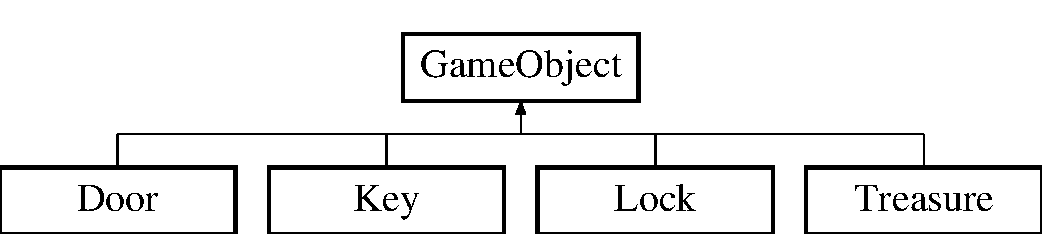
\includegraphics[height=2.000000cm]{classGameObject}
\end{center}
\end{figure}
\subsection*{\-Public \-Member \-Functions}
\begin{DoxyCompactItemize}
\item 
\hyperlink{classGameObject_a0996f1381d0512d9db0a89121e07335a}{\-Game\-Object} (\-Scene\-Manager $\ast$m\-Scene\-Mgr)
\item 
void \hyperlink{classGameObject_aa9a2c30e2cc2f6a7ddbb55d46dd9b45d}{place\-Object\-On\-W\-P} (\hyperlink{classWayPoint}{\-Way\-Point} $\ast$location)
\item 
\hyperlink{classWayPoint}{\-Way\-Point} $\ast$ \hyperlink{classGameObject_a0000c172fae6c5609ecd34ca0c335d8c}{get\-Trigger} ()
\item 
\hyperlink{classWayPoint}{\-Way\-Point} $\ast$ \hyperlink{classGameObject_a2e858346bacb7c0c078284dee036a927}{get\-W\-P} () const 
\item 
\-Game\-Object\-Type \hyperlink{classGameObject_a248b04d1269cb1d28c8b0cc2e886c1cb}{get\-Type} ()
\item 
virtual \-Game\-State \hyperlink{classGameObject_aa643df342c50df77f053eee2c703c619}{frame\-Event\-Queued} (\hyperlink{classWayPoint}{\-Way\-Point} $\ast$current\-W\-P, \-Game\-State gs)
\item 
void \hyperlink{classGameObject_a1f5648272592844af52605d1c83cc347}{set\-Visible} (bool val)
\item 
virtual void \hyperlink{classGameObject_ac3ab6708ce47b4ef8fd35d8bb43149dc}{init} (\hyperlink{classRoom}{\-Room} $\ast$\hyperlink{classGameObject_a9f63419cc03f2513f757a317a2e37557}{room})
\item 
void \hyperlink{classGameObject_afaea76d5acbb65e5f808bce98d8fda20}{reset\-Init} ()
\item 
bool \hyperlink{classGameObject_a5b3972654914248d6e757d409b596a96}{is\-Initialized} ()
\end{DoxyCompactItemize}
\subsection*{\-Protected \-Member \-Functions}
\begin{DoxyCompactItemize}
\item 
\hyperlink{classGameObject_a0348e3ee2e83d56eafca7a3547f432c4}{\-Game\-Object} ()
\end{DoxyCompactItemize}
\subsection*{\-Protected \-Attributes}
\begin{DoxyCompactItemize}
\item 
\-Scene\-Node $\ast$ \hyperlink{classGameObject_a44fbbf424125cebcb1e9a071946b6567}{my\-Node}
\item 
\hyperlink{classWayPoint}{\-Way\-Point} $\ast$ \hyperlink{classGameObject_ae8983dfdcfe7bcd2e81fe20a674bb3e6}{place}
\item 
\hyperlink{classWayPoint}{\-Way\-Point} $\ast$ \hyperlink{classGameObject_ace2db5f1940d0489b8766a77f0832069}{trigger}
\item 
\hyperlink{classRoom}{\-Room} $\ast$ \hyperlink{classGameObject_a9f63419cc03f2513f757a317a2e37557}{room}
\item 
bool \hyperlink{classGameObject_af98cecb661e1ffaa19d0d92041020319}{initialized}
\item 
\-Game\-Object\-Type \hyperlink{classGameObject_a6f5c85c8b3a4cb373efb1faa229fc9f3}{type}
\end{DoxyCompactItemize}


\subsection{\-Detailed \-Description}
\-Describes a generic game object. \-This class is an abstract description of a game object. \-It give some default functionality and is otherwise used to inherit the properties to its child classes\-: \hyperlink{classDoor}{\-Door}, \hyperlink{classKey}{\-Key}, \hyperlink{classTreasure}{\-Treasure} and \hyperlink{classLock}{\-Lock}. 

\subsection{\-Constructor \& \-Destructor \-Documentation}
\hypertarget{classGameObject_a0348e3ee2e83d56eafca7a3547f432c4}{\index{\-Game\-Object@{\-Game\-Object}!\-Game\-Object@{\-Game\-Object}}
\index{\-Game\-Object@{\-Game\-Object}!GameObject@{\-Game\-Object}}
\subsubsection[{\-Game\-Object}]{\setlength{\rightskip}{0pt plus 5cm}{\bf \-Game\-Object\-::\-Game\-Object} (
\begin{DoxyParamCaption}
{}
\end{DoxyParamCaption}
)\hspace{0.3cm}{\ttfamily  \mbox{[}inline, protected\mbox{]}}}}\label{classGameObject_a0348e3ee2e83d56eafca7a3547f432c4}
\-Default constructor. \-Not to be used outside class scope. \hypertarget{classGameObject_a0996f1381d0512d9db0a89121e07335a}{\index{\-Game\-Object@{\-Game\-Object}!\-Game\-Object@{\-Game\-Object}}
\index{\-Game\-Object@{\-Game\-Object}!GameObject@{\-Game\-Object}}
\subsubsection[{\-Game\-Object}]{\setlength{\rightskip}{0pt plus 5cm}{\bf \-Game\-Object\-::\-Game\-Object} (
\begin{DoxyParamCaption}
\item[{\-Scene\-Manager $\ast$}]{m\-Scene\-Mgr}
\end{DoxyParamCaption}
)\hspace{0.3cm}{\ttfamily  \mbox{[}inline\mbox{]}}}}\label{classGameObject_a0996f1381d0512d9db0a89121e07335a}
\-Do some standard initialization, needed by all object types. 

\subsection{\-Member \-Function \-Documentation}
\hypertarget{classGameObject_aa643df342c50df77f053eee2c703c619}{\index{\-Game\-Object@{\-Game\-Object}!frame\-Event\-Queued@{frame\-Event\-Queued}}
\index{frame\-Event\-Queued@{frame\-Event\-Queued}!GameObject@{\-Game\-Object}}
\subsubsection[{frame\-Event\-Queued}]{\setlength{\rightskip}{0pt plus 5cm}virtual \-Game\-State {\bf \-Game\-Object\-::frame\-Event\-Queued} (
\begin{DoxyParamCaption}
\item[{{\bf \-Way\-Point} $\ast$}]{current\-W\-P, }
\item[{\-Game\-State}]{gs}
\end{DoxyParamCaption}
)\hspace{0.3cm}{\ttfamily  \mbox{[}inline, virtual\mbox{]}}}}\label{classGameObject_aa643df342c50df77f053eee2c703c619}
\-Process the \-Game\-State and the current robot \hyperlink{classWayPoint}{\-Way\-Point} to derive the next \-Game\-State. 

\-Reimplemented in \hyperlink{classTreasure_a31089b8e8c8478e7c3e950b80bdb3785}{\-Treasure}, \hyperlink{classLock_a286412e42f06eff3d38b03028300cc01}{\-Lock}, \hyperlink{classDoor_a2e526ecea542d817e04771ed5487bebc}{\-Door}, and \hyperlink{classKey_a0ed28ed2112095183608b764e4453f9b}{\-Key}.

\hypertarget{classGameObject_a0000c172fae6c5609ecd34ca0c335d8c}{\index{\-Game\-Object@{\-Game\-Object}!get\-Trigger@{get\-Trigger}}
\index{get\-Trigger@{get\-Trigger}!GameObject@{\-Game\-Object}}
\subsubsection[{get\-Trigger}]{\setlength{\rightskip}{0pt plus 5cm}{\bf \-Way\-Point}$\ast$ {\bf \-Game\-Object\-::get\-Trigger} (
\begin{DoxyParamCaption}
{}
\end{DoxyParamCaption}
)\hspace{0.3cm}{\ttfamily  \mbox{[}inline\mbox{]}}}}\label{classGameObject_a0000c172fae6c5609ecd34ca0c335d8c}
\-Return the triggering \hyperlink{classWayPoint}{\-Way\-Point}. \hypertarget{classGameObject_a248b04d1269cb1d28c8b0cc2e886c1cb}{\index{\-Game\-Object@{\-Game\-Object}!get\-Type@{get\-Type}}
\index{get\-Type@{get\-Type}!GameObject@{\-Game\-Object}}
\subsubsection[{get\-Type}]{\setlength{\rightskip}{0pt plus 5cm}\-Game\-Object\-Type {\bf \-Game\-Object\-::get\-Type} (
\begin{DoxyParamCaption}
{}
\end{DoxyParamCaption}
)\hspace{0.3cm}{\ttfamily  \mbox{[}inline\mbox{]}}}}\label{classGameObject_a248b04d1269cb1d28c8b0cc2e886c1cb}
\-Return the type/use of this object. \hypertarget{classGameObject_a2e858346bacb7c0c078284dee036a927}{\index{\-Game\-Object@{\-Game\-Object}!get\-W\-P@{get\-W\-P}}
\index{get\-W\-P@{get\-W\-P}!GameObject@{\-Game\-Object}}
\subsubsection[{get\-W\-P}]{\setlength{\rightskip}{0pt plus 5cm}{\bf \-Way\-Point}$\ast$ {\bf \-Game\-Object\-::get\-W\-P} (
\begin{DoxyParamCaption}
{}
\end{DoxyParamCaption}
) const\hspace{0.3cm}{\ttfamily  \mbox{[}inline\mbox{]}}}}\label{classGameObject_a2e858346bacb7c0c078284dee036a927}
\-Return the location of the object. \hypertarget{classGameObject_ac3ab6708ce47b4ef8fd35d8bb43149dc}{\index{\-Game\-Object@{\-Game\-Object}!init@{init}}
\index{init@{init}!GameObject@{\-Game\-Object}}
\subsubsection[{init}]{\setlength{\rightskip}{0pt plus 5cm}virtual void {\bf \-Game\-Object\-::init} (
\begin{DoxyParamCaption}
\item[{{\bf \-Room} $\ast$}]{room}
\end{DoxyParamCaption}
)\hspace{0.3cm}{\ttfamily  \mbox{[}inline, virtual\mbox{]}}}}\label{classGameObject_ac3ab6708ce47b4ef8fd35d8bb43149dc}
(\-Re)initializes the \hyperlink{classGameObject}{\-Game\-Object} and the specified \hyperlink{classRoom}{\-Room} for a new game session. 

\-Reimplemented in \hyperlink{classTreasure_a5fcd48652f78053fcb0c84e6a89415fe}{\-Treasure}, \hyperlink{classLock_a357536468a884a9c2943b15b5fc6b39c}{\-Lock}, \hyperlink{classDoor_a6d9a56dd103f3f26b4beaf5682c22187}{\-Door}, and \hyperlink{classKey_a2c7e2bc5cc7099a52676ec8885142fde}{\-Key}.

\hypertarget{classGameObject_a5b3972654914248d6e757d409b596a96}{\index{\-Game\-Object@{\-Game\-Object}!is\-Initialized@{is\-Initialized}}
\index{is\-Initialized@{is\-Initialized}!GameObject@{\-Game\-Object}}
\subsubsection[{is\-Initialized}]{\setlength{\rightskip}{0pt plus 5cm}bool {\bf \-Game\-Object\-::is\-Initialized} (
\begin{DoxyParamCaption}
{}
\end{DoxyParamCaption}
)\hspace{0.3cm}{\ttfamily  \mbox{[}inline\mbox{]}}}}\label{classGameObject_a5b3972654914248d6e757d409b596a96}
\-Return if the object was initialized with init(...). \hypertarget{classGameObject_aa9a2c30e2cc2f6a7ddbb55d46dd9b45d}{\index{\-Game\-Object@{\-Game\-Object}!place\-Object\-On\-W\-P@{place\-Object\-On\-W\-P}}
\index{place\-Object\-On\-W\-P@{place\-Object\-On\-W\-P}!GameObject@{\-Game\-Object}}
\subsubsection[{place\-Object\-On\-W\-P}]{\setlength{\rightskip}{0pt plus 5cm}void {\bf \-Game\-Object\-::place\-Object\-On\-W\-P} (
\begin{DoxyParamCaption}
\item[{{\bf \-Way\-Point} $\ast$}]{location}
\end{DoxyParamCaption}
)\hspace{0.3cm}{\ttfamily  \mbox{[}inline\mbox{]}}}}\label{classGameObject_aa9a2c30e2cc2f6a7ddbb55d46dd9b45d}
\-Places the object on the specified \hyperlink{classWayPoint}{\-Way\-Point} and sets the scene node's visibility to true. \hypertarget{classGameObject_afaea76d5acbb65e5f808bce98d8fda20}{\index{\-Game\-Object@{\-Game\-Object}!reset\-Init@{reset\-Init}}
\index{reset\-Init@{reset\-Init}!GameObject@{\-Game\-Object}}
\subsubsection[{reset\-Init}]{\setlength{\rightskip}{0pt plus 5cm}void {\bf \-Game\-Object\-::reset\-Init} (
\begin{DoxyParamCaption}
{}
\end{DoxyParamCaption}
)\hspace{0.3cm}{\ttfamily  \mbox{[}inline\mbox{]}}}}\label{classGameObject_afaea76d5acbb65e5f808bce98d8fda20}
\-Make the object ready for reinitialization. \-Has to be called before init every time after the first. \hypertarget{classGameObject_a1f5648272592844af52605d1c83cc347}{\index{\-Game\-Object@{\-Game\-Object}!set\-Visible@{set\-Visible}}
\index{set\-Visible@{set\-Visible}!GameObject@{\-Game\-Object}}
\subsubsection[{set\-Visible}]{\setlength{\rightskip}{0pt plus 5cm}void {\bf \-Game\-Object\-::set\-Visible} (
\begin{DoxyParamCaption}
\item[{bool}]{val}
\end{DoxyParamCaption}
)\hspace{0.3cm}{\ttfamily  \mbox{[}inline\mbox{]}}}}\label{classGameObject_a1f5648272592844af52605d1c83cc347}
\-Sets the scene node visibility. 

\subsection{\-Member \-Data \-Documentation}
\hypertarget{classGameObject_af98cecb661e1ffaa19d0d92041020319}{\index{\-Game\-Object@{\-Game\-Object}!initialized@{initialized}}
\index{initialized@{initialized}!GameObject@{\-Game\-Object}}
\subsubsection[{initialized}]{\setlength{\rightskip}{0pt plus 5cm}bool {\bf \-Game\-Object\-::initialized}\hspace{0.3cm}{\ttfamily  \mbox{[}protected\mbox{]}}}}\label{classGameObject_af98cecb661e1ffaa19d0d92041020319}
\-Remember if this object was initialized with the init(...) method. \hypertarget{classGameObject_a44fbbf424125cebcb1e9a071946b6567}{\index{\-Game\-Object@{\-Game\-Object}!my\-Node@{my\-Node}}
\index{my\-Node@{my\-Node}!GameObject@{\-Game\-Object}}
\subsubsection[{my\-Node}]{\setlength{\rightskip}{0pt plus 5cm}\-Scene\-Node$\ast$ {\bf \-Game\-Object\-::my\-Node}\hspace{0.3cm}{\ttfamily  \mbox{[}protected\mbox{]}}}}\label{classGameObject_a44fbbf424125cebcb1e9a071946b6567}
\-Each \hyperlink{classGameObject}{\-Game\-Object} has its own \-Scene\-Node. \hypertarget{classGameObject_ae8983dfdcfe7bcd2e81fe20a674bb3e6}{\index{\-Game\-Object@{\-Game\-Object}!place@{place}}
\index{place@{place}!GameObject@{\-Game\-Object}}
\subsubsection[{place}]{\setlength{\rightskip}{0pt plus 5cm}{\bf \-Way\-Point}$\ast$ {\bf \-Game\-Object\-::place}\hspace{0.3cm}{\ttfamily  \mbox{[}protected\mbox{]}}}}\label{classGameObject_ae8983dfdcfe7bcd2e81fe20a674bb3e6}
\-Remember the waypoint this object is placed at. \hypertarget{classGameObject_a9f63419cc03f2513f757a317a2e37557}{\index{\-Game\-Object@{\-Game\-Object}!room@{room}}
\index{room@{room}!GameObject@{\-Game\-Object}}
\subsubsection[{room}]{\setlength{\rightskip}{0pt plus 5cm}{\bf \-Room}$\ast$ {\bf \-Game\-Object\-::room}\hspace{0.3cm}{\ttfamily  \mbox{[}protected\mbox{]}}}}\label{classGameObject_a9f63419cc03f2513f757a317a2e37557}
\-The room this object is associated with. \hypertarget{classGameObject_ace2db5f1940d0489b8766a77f0832069}{\index{\-Game\-Object@{\-Game\-Object}!trigger@{trigger}}
\index{trigger@{trigger}!GameObject@{\-Game\-Object}}
\subsubsection[{trigger}]{\setlength{\rightskip}{0pt plus 5cm}{\bf \-Way\-Point}$\ast$ {\bf \-Game\-Object\-::trigger}\hspace{0.3cm}{\ttfamily  \mbox{[}protected\mbox{]}}}}\label{classGameObject_ace2db5f1940d0489b8766a77f0832069}
\-The waypoint this object responds to (the one that causes the \-Game\-State to change). \hypertarget{classGameObject_a6f5c85c8b3a4cb373efb1faa229fc9f3}{\index{\-Game\-Object@{\-Game\-Object}!type@{type}}
\index{type@{type}!GameObject@{\-Game\-Object}}
\subsubsection[{type}]{\setlength{\rightskip}{0pt plus 5cm}\-Game\-Object\-Type {\bf \-Game\-Object\-::type}\hspace{0.3cm}{\ttfamily  \mbox{[}protected\mbox{]}}}}\label{classGameObject_a6f5c85c8b3a4cb373efb1faa229fc9f3}
\-Type of this object. \-Set in the child class. 

\-The documentation for this class was generated from the following file\-:\begin{DoxyCompactItemize}
\item 
roculus/include/\-Game\-Object.\-h\end{DoxyCompactItemize}

\hypertarget{classGlobalMap}{\section{\-Global\-Map \-Class \-Reference}
\label{classGlobalMap}\index{\-Global\-Map@{\-Global\-Map}}
}


\-Utility class for the 2\-D map. \-This class handles the 2\-D map in the scene.  




{\ttfamily \#include $<$\-Global\-Map.\-h$>$}

\subsection*{\-Public \-Member \-Functions}
\begin{DoxyCompactItemize}
\item 
\hyperlink{classGlobalMap_a308deb321ce23efd983e1b531610fe74}{\-Global\-Map} (\-Scene\-Manager $\ast$)
\item 
\hyperlink{classGlobalMap_a72b4215462449c75b7758df8f6b34097}{$\sim$\-Global\-Map} ()
\item 
void \hyperlink{classGlobalMap_aeb2b21e3ddde44e8999837dd69445d9d}{insert\-W\-H\-R} (uint32, uint32, \-Real)
\item 
void \hyperlink{classGlobalMap_a1563668430b40d8714d1b276f54c544a}{set\-Origin} (\-Vector3)
\item 
void \hyperlink{classGlobalMap_aa3bb0eeddafa5949d86c3324ada09f6f}{include\-Map} (const \-Image \&)
\item 
void \hyperlink{classGlobalMap_a355f582edb923cc85a6ca3967f6cd70e}{flip\-Visibility} ()
\item 
\-Real \hyperlink{classGlobalMap_add6bc1a0cd3c67142d4e0839b285a03b}{get\-Width} ()
\item 
\-Real \hyperlink{classGlobalMap_a470de4de22c822d7fbb448775bd51be4}{get\-Height} ()
\item 
\-Real \hyperlink{classGlobalMap_a5b489c16007ddad138c9ad4b5ed9c4cf}{get\-Resolution} ()
\item 
\-Vector3 \hyperlink{classGlobalMap_a6263c44606f891c5ed167e58a7690597}{get\-Origin} ()
\end{DoxyCompactItemize}
\subsection*{\-Protected \-Attributes}
\begin{DoxyCompactItemize}
\item 
\-Real \hyperlink{classGlobalMap_adbd369e87c136942c600d7675595ebd7}{width}
\item 
\-Real \hyperlink{classGlobalMap_a8c44af901d0f19fb8a57845d03e24063}{height}
\item 
\-Real \hyperlink{classGlobalMap_a0bfaceb4b03dd0c79179f627565d3a8a}{resolution}
\item 
\-Vector3 \hyperlink{classGlobalMap_a79a33b5d851acd03cff2d74b1aaaf020}{origin}
\item 
\-Scene\-Manager $\ast$ \hyperlink{classGlobalMap_a58e2848e9c5f3abe6effaf12176c2c8e}{m\-Scene\-Mgr}
\item 
\-Manual\-Object $\ast$ \hyperlink{classGlobalMap_a59b1001eec405852745ecf64a47915be}{m\-Map\-Obj}
\item 
\-Scene\-Node $\ast$ \hyperlink{classGlobalMap_a3ef2cbe2c69a7257fbf17ef338e679c1}{p\-Scene\-Node}
\end{DoxyCompactItemize}


\subsection{\-Detailed \-Description}
\-Utility class for the 2\-D map. \-This class handles the 2\-D map in the scene. 

$<$ 

\subsection{\-Constructor \& \-Destructor \-Documentation}
\hypertarget{classGlobalMap_a308deb321ce23efd983e1b531610fe74}{\index{\-Global\-Map@{\-Global\-Map}!\-Global\-Map@{\-Global\-Map}}
\index{\-Global\-Map@{\-Global\-Map}!GlobalMap@{\-Global\-Map}}
\subsubsection[{\-Global\-Map}]{\setlength{\rightskip}{0pt plus 5cm}{\bf \-Global\-Map\-::\-Global\-Map} (
\begin{DoxyParamCaption}
\item[{\-Scene\-Manager $\ast$}]{}
\end{DoxyParamCaption}
)}}\label{classGlobalMap_a308deb321ce23efd983e1b531610fe74}
\-Use this constructor to initialize the object! \hypertarget{classGlobalMap_a72b4215462449c75b7758df8f6b34097}{\index{\-Global\-Map@{\-Global\-Map}!$\sim$\-Global\-Map@{$\sim$\-Global\-Map}}
\index{$\sim$\-Global\-Map@{$\sim$\-Global\-Map}!GlobalMap@{\-Global\-Map}}
\subsubsection[{$\sim$\-Global\-Map}]{\setlength{\rightskip}{0pt plus 5cm}{\bf \-Global\-Map\-::$\sim$\-Global\-Map} (
\begin{DoxyParamCaption}
{}
\end{DoxyParamCaption}
)}}\label{classGlobalMap_a72b4215462449c75b7758df8f6b34097}
\-Default destructor. 

\subsection{\-Member \-Function \-Documentation}
\hypertarget{classGlobalMap_a355f582edb923cc85a6ca3967f6cd70e}{\index{\-Global\-Map@{\-Global\-Map}!flip\-Visibility@{flip\-Visibility}}
\index{flip\-Visibility@{flip\-Visibility}!GlobalMap@{\-Global\-Map}}
\subsubsection[{flip\-Visibility}]{\setlength{\rightskip}{0pt plus 5cm}void {\bf \-Global\-Map\-::flip\-Visibility} (
\begin{DoxyParamCaption}
{}
\end{DoxyParamCaption}
)}}\label{classGlobalMap_a355f582edb923cc85a6ca3967f6cd70e}
\-Trigger the visibility of the map. \hypertarget{classGlobalMap_a470de4de22c822d7fbb448775bd51be4}{\index{\-Global\-Map@{\-Global\-Map}!get\-Height@{get\-Height}}
\index{get\-Height@{get\-Height}!GlobalMap@{\-Global\-Map}}
\subsubsection[{get\-Height}]{\setlength{\rightskip}{0pt plus 5cm}\-Real {\bf \-Global\-Map\-::get\-Height} (
\begin{DoxyParamCaption}
{}
\end{DoxyParamCaption}
)}}\label{classGlobalMap_a470de4de22c822d7fbb448775bd51be4}
\-Return the height(depth) of the map. \hypertarget{classGlobalMap_a6263c44606f891c5ed167e58a7690597}{\index{\-Global\-Map@{\-Global\-Map}!get\-Origin@{get\-Origin}}
\index{get\-Origin@{get\-Origin}!GlobalMap@{\-Global\-Map}}
\subsubsection[{get\-Origin}]{\setlength{\rightskip}{0pt plus 5cm}\-Vector3 {\bf \-Global\-Map\-::get\-Origin} (
\begin{DoxyParamCaption}
{}
\end{DoxyParamCaption}
)}}\label{classGlobalMap_a6263c44606f891c5ed167e58a7690597}
\-Return the origin of the map. \hypertarget{classGlobalMap_a5b489c16007ddad138c9ad4b5ed9c4cf}{\index{\-Global\-Map@{\-Global\-Map}!get\-Resolution@{get\-Resolution}}
\index{get\-Resolution@{get\-Resolution}!GlobalMap@{\-Global\-Map}}
\subsubsection[{get\-Resolution}]{\setlength{\rightskip}{0pt plus 5cm}\-Real {\bf \-Global\-Map\-::get\-Resolution} (
\begin{DoxyParamCaption}
{}
\end{DoxyParamCaption}
)}}\label{classGlobalMap_a5b489c16007ddad138c9ad4b5ed9c4cf}
\-Return the resolution of the map. \hypertarget{classGlobalMap_add6bc1a0cd3c67142d4e0839b285a03b}{\index{\-Global\-Map@{\-Global\-Map}!get\-Width@{get\-Width}}
\index{get\-Width@{get\-Width}!GlobalMap@{\-Global\-Map}}
\subsubsection[{get\-Width}]{\setlength{\rightskip}{0pt plus 5cm}\-Real {\bf \-Global\-Map\-::get\-Width} (
\begin{DoxyParamCaption}
{}
\end{DoxyParamCaption}
)}}\label{classGlobalMap_add6bc1a0cd3c67142d4e0839b285a03b}
\-Return the width of the map. \hypertarget{classGlobalMap_aa3bb0eeddafa5949d86c3324ada09f6f}{\index{\-Global\-Map@{\-Global\-Map}!include\-Map@{include\-Map}}
\index{include\-Map@{include\-Map}!GlobalMap@{\-Global\-Map}}
\subsubsection[{include\-Map}]{\setlength{\rightskip}{0pt plus 5cm}void {\bf \-Global\-Map\-::include\-Map} (
\begin{DoxyParamCaption}
\item[{const \-Image \&}]{}
\end{DoxyParamCaption}
)}}\label{classGlobalMap_aa3bb0eeddafa5949d86c3324ada09f6f}
\-Given the image, create the map plane and texture it with the image. \-Place the scene node in the world. \hypertarget{classGlobalMap_aeb2b21e3ddde44e8999837dd69445d9d}{\index{\-Global\-Map@{\-Global\-Map}!insert\-W\-H\-R@{insert\-W\-H\-R}}
\index{insert\-W\-H\-R@{insert\-W\-H\-R}!GlobalMap@{\-Global\-Map}}
\subsubsection[{insert\-W\-H\-R}]{\setlength{\rightskip}{0pt plus 5cm}void {\bf \-Global\-Map\-::insert\-W\-H\-R} (
\begin{DoxyParamCaption}
\item[{uint32}]{, }
\item[{uint32}]{, }
\item[{\-Real}]{}
\end{DoxyParamCaption}
)}}\label{classGlobalMap_aeb2b21e3ddde44e8999837dd69445d9d}
\-Set the width, height(depth), and resolution of the map-\/image. \hypertarget{classGlobalMap_a1563668430b40d8714d1b276f54c544a}{\index{\-Global\-Map@{\-Global\-Map}!set\-Origin@{set\-Origin}}
\index{set\-Origin@{set\-Origin}!GlobalMap@{\-Global\-Map}}
\subsubsection[{set\-Origin}]{\setlength{\rightskip}{0pt plus 5cm}void {\bf \-Global\-Map\-::set\-Origin} (
\begin{DoxyParamCaption}
\item[{\-Vector3}]{}
\end{DoxyParamCaption}
)}}\label{classGlobalMap_a1563668430b40d8714d1b276f54c544a}
\-Set the origin of the map. 

\subsection{\-Member \-Data \-Documentation}
\hypertarget{classGlobalMap_a8c44af901d0f19fb8a57845d03e24063}{\index{\-Global\-Map@{\-Global\-Map}!height@{height}}
\index{height@{height}!GlobalMap@{\-Global\-Map}}
\subsubsection[{height}]{\setlength{\rightskip}{0pt plus 5cm}\-Real {\bf \-Global\-Map\-::height}\hspace{0.3cm}{\ttfamily  \mbox{[}protected\mbox{]}}}}\label{classGlobalMap_a8c44af901d0f19fb8a57845d03e24063}
\-The height(depth) of the map. \hypertarget{classGlobalMap_a59b1001eec405852745ecf64a47915be}{\index{\-Global\-Map@{\-Global\-Map}!m\-Map\-Obj@{m\-Map\-Obj}}
\index{m\-Map\-Obj@{m\-Map\-Obj}!GlobalMap@{\-Global\-Map}}
\subsubsection[{m\-Map\-Obj}]{\setlength{\rightskip}{0pt plus 5cm}\-Manual\-Object$\ast$ {\bf \-Global\-Map\-::m\-Map\-Obj}\hspace{0.3cm}{\ttfamily  \mbox{[}protected\mbox{]}}}}\label{classGlobalMap_a59b1001eec405852745ecf64a47915be}
\-The manual object used to create the plane. \hypertarget{classGlobalMap_a58e2848e9c5f3abe6effaf12176c2c8e}{\index{\-Global\-Map@{\-Global\-Map}!m\-Scene\-Mgr@{m\-Scene\-Mgr}}
\index{m\-Scene\-Mgr@{m\-Scene\-Mgr}!GlobalMap@{\-Global\-Map}}
\subsubsection[{m\-Scene\-Mgr}]{\setlength{\rightskip}{0pt plus 5cm}\-Scene\-Manager$\ast$ {\bf \-Global\-Map\-::m\-Scene\-Mgr}\hspace{0.3cm}{\ttfamily  \mbox{[}protected\mbox{]}}}}\label{classGlobalMap_a58e2848e9c5f3abe6effaf12176c2c8e}
\-The scene manager. \hypertarget{classGlobalMap_a79a33b5d851acd03cff2d74b1aaaf020}{\index{\-Global\-Map@{\-Global\-Map}!origin@{origin}}
\index{origin@{origin}!GlobalMap@{\-Global\-Map}}
\subsubsection[{origin}]{\setlength{\rightskip}{0pt plus 5cm}\-Vector3 {\bf \-Global\-Map\-::origin}\hspace{0.3cm}{\ttfamily  \mbox{[}protected\mbox{]}}}}\label{classGlobalMap_a79a33b5d851acd03cff2d74b1aaaf020}
\-The origin of the map. \hypertarget{classGlobalMap_a3ef2cbe2c69a7257fbf17ef338e679c1}{\index{\-Global\-Map@{\-Global\-Map}!p\-Scene\-Node@{p\-Scene\-Node}}
\index{p\-Scene\-Node@{p\-Scene\-Node}!GlobalMap@{\-Global\-Map}}
\subsubsection[{p\-Scene\-Node}]{\setlength{\rightskip}{0pt plus 5cm}\-Scene\-Node$\ast$ {\bf \-Global\-Map\-::p\-Scene\-Node}\hspace{0.3cm}{\ttfamily  \mbox{[}protected\mbox{]}}}}\label{classGlobalMap_a3ef2cbe2c69a7257fbf17ef338e679c1}
\-The scene node that holds the map. \hypertarget{classGlobalMap_a0bfaceb4b03dd0c79179f627565d3a8a}{\index{\-Global\-Map@{\-Global\-Map}!resolution@{resolution}}
\index{resolution@{resolution}!GlobalMap@{\-Global\-Map}}
\subsubsection[{resolution}]{\setlength{\rightskip}{0pt plus 5cm}\-Real {\bf \-Global\-Map\-::resolution}\hspace{0.3cm}{\ttfamily  \mbox{[}protected\mbox{]}}}}\label{classGlobalMap_a0bfaceb4b03dd0c79179f627565d3a8a}
\-The reolution of the map. \hypertarget{classGlobalMap_adbd369e87c136942c600d7675595ebd7}{\index{\-Global\-Map@{\-Global\-Map}!width@{width}}
\index{width@{width}!GlobalMap@{\-Global\-Map}}
\subsubsection[{width}]{\setlength{\rightskip}{0pt plus 5cm}\-Real {\bf \-Global\-Map\-::width}\hspace{0.3cm}{\ttfamily  \mbox{[}protected\mbox{]}}}}\label{classGlobalMap_adbd369e87c136942c600d7675595ebd7}
\-The width of the map. 

\-The documentation for this class was generated from the following file\-:\begin{DoxyCompactItemize}
\item 
roculus/include/\-Global\-Map.\-h\end{DoxyCompactItemize}

\hypertarget{classKey}{\section{\-Key \-Class \-Reference}
\label{classKey}\index{\-Key@{\-Key}}
}


\-Represents a \hyperlink{classKey}{\-Key} in a \hyperlink{classGame}{\-Game}. \-This class is a more detailed description of the \hyperlink{classGameObject}{\-Game\-Object} \hyperlink{classKey}{\-Key}. \-It specifies how to display and what to do with a key.  




{\ttfamily \#include $<$\-Key.\-h$>$}

\-Inheritance diagram for \-Key\-:\begin{figure}[H]
\begin{center}
\leavevmode
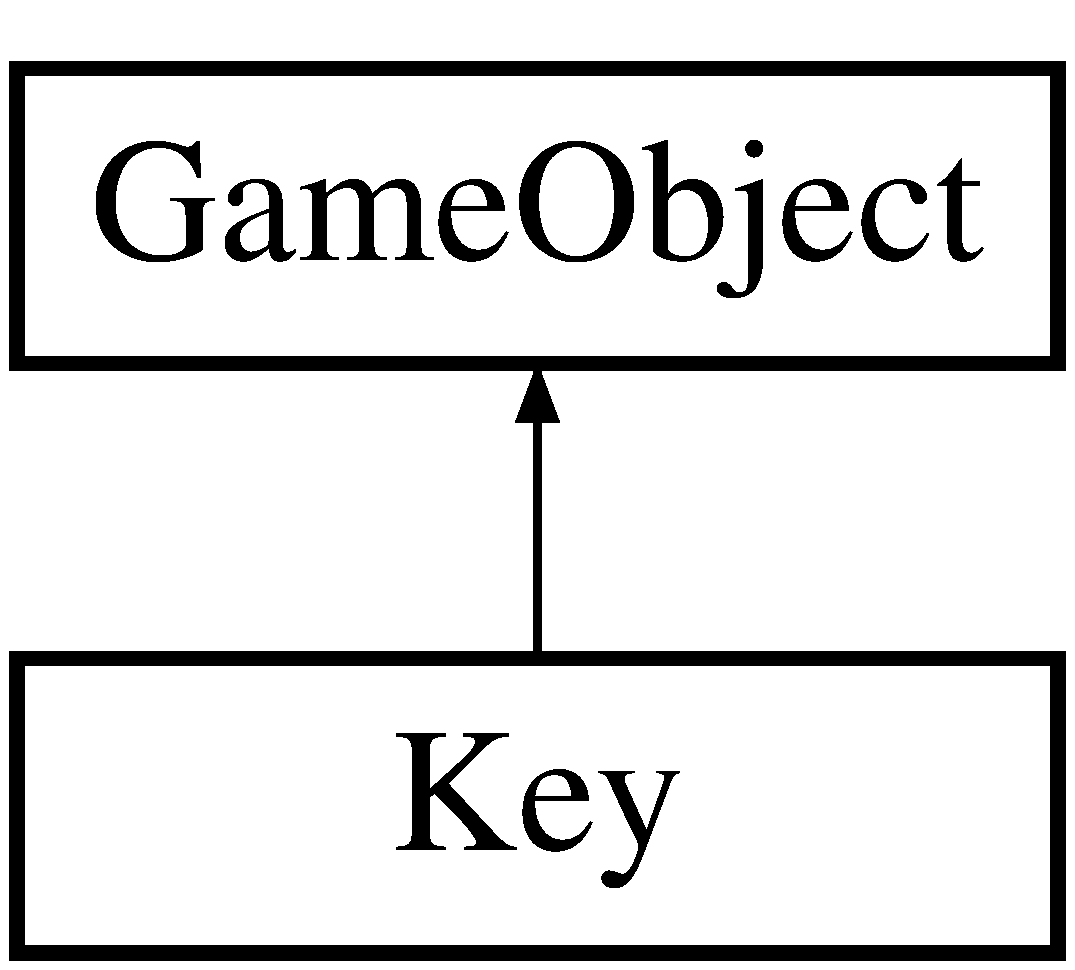
\includegraphics[height=2.000000cm]{classKey}
\end{center}
\end{figure}
\subsection*{\-Public \-Member \-Functions}
\begin{DoxyCompactItemize}
\item 
\hyperlink{classKey_ae07b933c3599eb3d74eb1b61f91066fb}{\-Key} (\-Scene\-Manager $\ast$)
\item 
virtual \-Game\-State \hyperlink{classKey_a0ed28ed2112095183608b764e4453f9b}{frame\-Event\-Queued} (\hyperlink{classWayPoint}{\-Way\-Point} $\ast$current\-W\-P, \-Game\-State gs)
\item 
virtual void \hyperlink{classKey_a2c7e2bc5cc7099a52676ec8885142fde}{init} (\hyperlink{classRoom}{\-Room} $\ast$\hyperlink{classGameObject_a9f63419cc03f2513f757a317a2e37557}{room})
\end{DoxyCompactItemize}
\subsection*{\-Protected \-Member \-Functions}
\begin{DoxyCompactItemize}
\item 
\hyperlink{classKey_a22e51dbebb18c1d33ee8bba93a1b3b4d}{\-Key} ()
\end{DoxyCompactItemize}
\subsection*{\-Protected \-Attributes}
\begin{DoxyCompactItemize}
\item 
bool \hyperlink{classKey_a030a1f58ce504bb15802f19287252de9}{found}
\end{DoxyCompactItemize}


\subsection{\-Detailed \-Description}
\-Represents a \hyperlink{classKey}{\-Key} in a \hyperlink{classGame}{\-Game}. \-This class is a more detailed description of the \hyperlink{classGameObject}{\-Game\-Object} \hyperlink{classKey}{\-Key}. \-It specifies how to display and what to do with a key. 

\subsection{\-Constructor \& \-Destructor \-Documentation}
\hypertarget{classKey_a22e51dbebb18c1d33ee8bba93a1b3b4d}{\index{\-Key@{\-Key}!\-Key@{\-Key}}
\index{\-Key@{\-Key}!Key@{\-Key}}
\subsubsection[{\-Key}]{\setlength{\rightskip}{0pt plus 5cm}{\bf \-Key\-::\-Key} (
\begin{DoxyParamCaption}
{}
\end{DoxyParamCaption}
)\hspace{0.3cm}{\ttfamily  \mbox{[}protected\mbox{]}}}}\label{classKey_a22e51dbebb18c1d33ee8bba93a1b3b4d}
\-Default constructor. \-Not to be used outside class scope. \hypertarget{classKey_ae07b933c3599eb3d74eb1b61f91066fb}{\index{\-Key@{\-Key}!\-Key@{\-Key}}
\index{\-Key@{\-Key}!Key@{\-Key}}
\subsubsection[{\-Key}]{\setlength{\rightskip}{0pt plus 5cm}{\bf \-Key\-::\-Key} (
\begin{DoxyParamCaption}
\item[{\-Scene\-Manager $\ast$}]{}
\end{DoxyParamCaption}
)}}\label{classKey_ae07b933c3599eb3d74eb1b61f91066fb}
\-Initializes the key object and sets it up for display. 

\subsection{\-Member \-Function \-Documentation}
\hypertarget{classKey_a0ed28ed2112095183608b764e4453f9b}{\index{\-Key@{\-Key}!frame\-Event\-Queued@{frame\-Event\-Queued}}
\index{frame\-Event\-Queued@{frame\-Event\-Queued}!Key@{\-Key}}
\subsubsection[{frame\-Event\-Queued}]{\setlength{\rightskip}{0pt plus 5cm}virtual \-Game\-State {\bf \-Key\-::frame\-Event\-Queued} (
\begin{DoxyParamCaption}
\item[{{\bf \-Way\-Point} $\ast$}]{current\-W\-P, }
\item[{\-Game\-State}]{gs}
\end{DoxyParamCaption}
)\hspace{0.3cm}{\ttfamily  \mbox{[}virtual\mbox{]}}}}\label{classKey_a0ed28ed2112095183608b764e4453f9b}
\-Reimplements \hyperlink{classGameObject_aa643df342c50df77f053eee2c703c619}{\-Game\-Object\-::frame\-Event\-Queued}(...). \-Processes the current robot \hyperlink{classWayPoint}{\-Way\-Point} and \-Game\-State to derive if the next state is effected by this key. 

\-Reimplemented from \hyperlink{classGameObject_aa643df342c50df77f053eee2c703c619}{\-Game\-Object}.

\hypertarget{classKey_a2c7e2bc5cc7099a52676ec8885142fde}{\index{\-Key@{\-Key}!init@{init}}
\index{init@{init}!Key@{\-Key}}
\subsubsection[{init}]{\setlength{\rightskip}{0pt plus 5cm}virtual void {\bf \-Key\-::init} (
\begin{DoxyParamCaption}
\item[{{\bf \-Room} $\ast$}]{room}
\end{DoxyParamCaption}
)\hspace{0.3cm}{\ttfamily  \mbox{[}virtual\mbox{]}}}}\label{classKey_a2c7e2bc5cc7099a52676ec8885142fde}
\-Reinitializes the object for a new game session. 

\-Reimplemented from \hyperlink{classGameObject_ac3ab6708ce47b4ef8fd35d8bb43149dc}{\-Game\-Object}.



\subsection{\-Member \-Data \-Documentation}
\hypertarget{classKey_a030a1f58ce504bb15802f19287252de9}{\index{\-Key@{\-Key}!found@{found}}
\index{found@{found}!Key@{\-Key}}
\subsubsection[{found}]{\setlength{\rightskip}{0pt plus 5cm}bool {\bf \-Key\-::found}\hspace{0.3cm}{\ttfamily  \mbox{[}protected\mbox{]}}}}\label{classKey_a030a1f58ce504bb15802f19287252de9}
\-Was this key found, or not? 

\-The documentation for this class was generated from the following file\-:\begin{DoxyCompactItemize}
\item 
roculus/include/\-Key.\-h\end{DoxyCompactItemize}

\hypertarget{classLock}{\section{\-Lock \-Class \-Reference}
\label{classLock}\index{\-Lock@{\-Lock}}
}


\-Describes a \hyperlink{classLock}{\-Lock} in a \hyperlink{classGame}{\-Game}. \-This class specifies the details to display a lock and implements its behaviour.  




{\ttfamily \#include $<$\-Lock.\-h$>$}

\-Inheritance diagram for \-Lock\-:\begin{figure}[H]
\begin{center}
\leavevmode
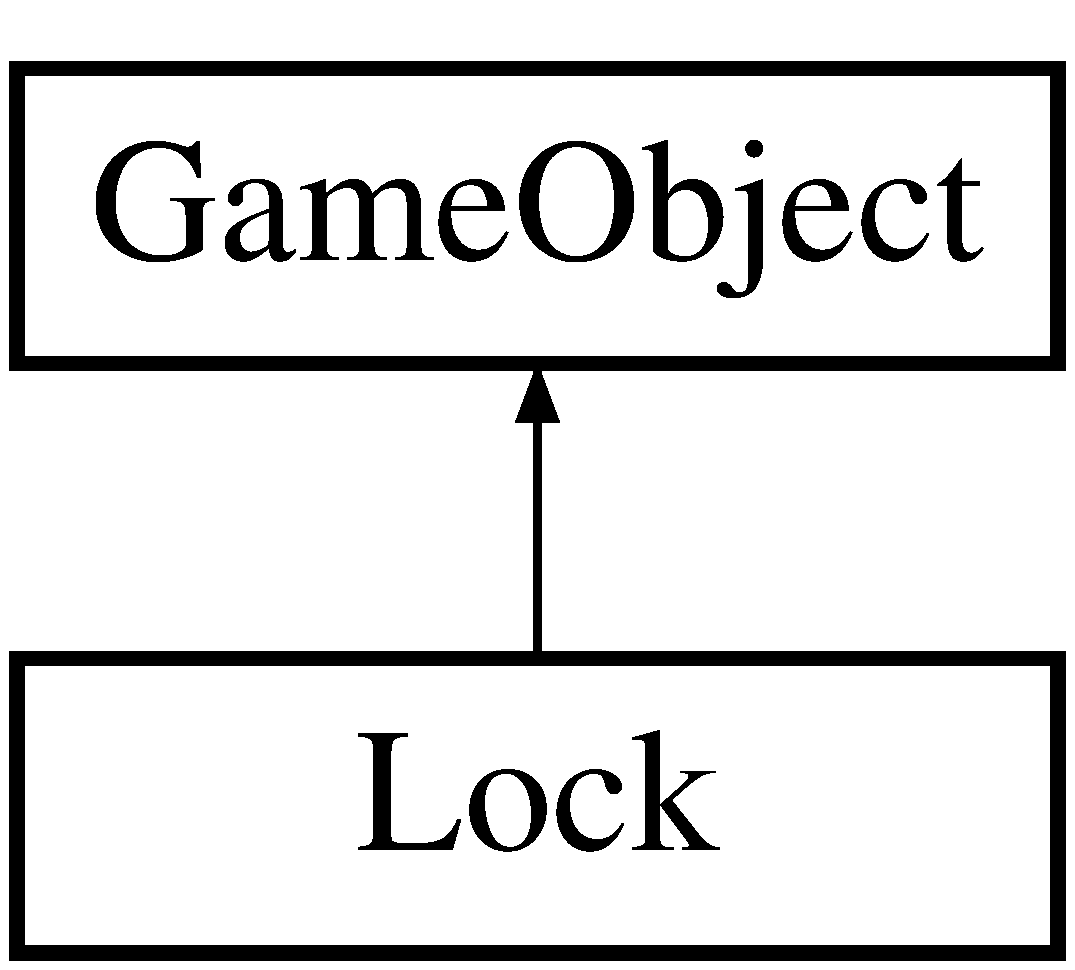
\includegraphics[height=2.000000cm]{classLock}
\end{center}
\end{figure}
\subsection*{\-Public \-Member \-Functions}
\begin{DoxyCompactItemize}
\item 
\hyperlink{classLock_aae94a6576b49afad57330bf537a8edfc}{\-Lock} (\-Scene\-Manager $\ast$, int)
\item 
virtual \-Game\-State \hyperlink{classLock_a286412e42f06eff3d38b03028300cc01}{frame\-Event\-Queued} (\hyperlink{classWayPoint}{\-Way\-Point} $\ast$current\-W\-P, \-Game\-State gs)
\item 
virtual void \hyperlink{classLock_a357536468a884a9c2943b15b5fc6b39c}{init} (\hyperlink{classRoom}{\-Room} $\ast$\hyperlink{classGameObject_a9f63419cc03f2513f757a317a2e37557}{room})
\end{DoxyCompactItemize}
\subsection*{\-Protected \-Member \-Functions}
\begin{DoxyCompactItemize}
\item 
\hyperlink{classLock_a9944623567d8138b95e74fadc7190adb}{\-Lock} ()
\end{DoxyCompactItemize}
\subsection*{\-Protected \-Attributes}
\begin{DoxyCompactItemize}
\item 
\-Game\-State \hyperlink{classLock_aa3796f83850ec610bf5f34ee05b6bdfd}{react}
\item 
\-Entity $\ast$ \hyperlink{classLock_ab92f200ca97e214793f439bfa512159c}{ent}
\item 
int \hyperlink{classLock_a7d5ea9a673fdfc9378bf54633a3c7885}{idx}
\item 
bool \hyperlink{classLock_a3f84294da55d52499fe63886b4673d6f}{locked}
\end{DoxyCompactItemize}


\subsection{\-Detailed \-Description}
\-Describes a \hyperlink{classLock}{\-Lock} in a \hyperlink{classGame}{\-Game}. \-This class specifies the details to display a lock and implements its behaviour. 

\subsection{\-Constructor \& \-Destructor \-Documentation}
\hypertarget{classLock_a9944623567d8138b95e74fadc7190adb}{\index{\-Lock@{\-Lock}!\-Lock@{\-Lock}}
\index{\-Lock@{\-Lock}!Lock@{\-Lock}}
\subsubsection[{\-Lock}]{\setlength{\rightskip}{0pt plus 5cm}{\bf \-Lock\-::\-Lock} (
\begin{DoxyParamCaption}
{}
\end{DoxyParamCaption}
)\hspace{0.3cm}{\ttfamily  \mbox{[}inline, protected\mbox{]}}}}\label{classLock_a9944623567d8138b95e74fadc7190adb}
\-Default constructor. \-Not to be used outside class scope. \hypertarget{classLock_aae94a6576b49afad57330bf537a8edfc}{\index{\-Lock@{\-Lock}!\-Lock@{\-Lock}}
\index{\-Lock@{\-Lock}!Lock@{\-Lock}}
\subsubsection[{\-Lock}]{\setlength{\rightskip}{0pt plus 5cm}{\bf \-Lock\-::\-Lock} (
\begin{DoxyParamCaption}
\item[{\-Scene\-Manager $\ast$}]{, }
\item[{int}]{}
\end{DoxyParamCaption}
)}}\label{classLock_aae94a6576b49afad57330bf537a8edfc}
\-Initialize the \hyperlink{classLock}{\-Lock} with the scene manager (to set up the display) and the number of the key to respond to for the game logic. 

\subsection{\-Member \-Function \-Documentation}
\hypertarget{classLock_a286412e42f06eff3d38b03028300cc01}{\index{\-Lock@{\-Lock}!frame\-Event\-Queued@{frame\-Event\-Queued}}
\index{frame\-Event\-Queued@{frame\-Event\-Queued}!Lock@{\-Lock}}
\subsubsection[{frame\-Event\-Queued}]{\setlength{\rightskip}{0pt plus 5cm}virtual \-Game\-State {\bf \-Lock\-::frame\-Event\-Queued} (
\begin{DoxyParamCaption}
\item[{{\bf \-Way\-Point} $\ast$}]{current\-W\-P, }
\item[{\-Game\-State}]{gs}
\end{DoxyParamCaption}
)\hspace{0.3cm}{\ttfamily  \mbox{[}virtual\mbox{]}}}}\label{classLock_a286412e42f06eff3d38b03028300cc01}
\-Reimplements \hyperlink{classGameObject_aa643df342c50df77f053eee2c703c619}{\-Game\-Object\-::frame\-Event\-Queued}(...). \-Given the inputs, derive next \-Game\-State. 

\-Reimplemented from \hyperlink{classGameObject_aa643df342c50df77f053eee2c703c619}{\-Game\-Object}.

\hypertarget{classLock_a357536468a884a9c2943b15b5fc6b39c}{\index{\-Lock@{\-Lock}!init@{init}}
\index{init@{init}!Lock@{\-Lock}}
\subsubsection[{init}]{\setlength{\rightskip}{0pt plus 5cm}virtual void {\bf \-Lock\-::init} (
\begin{DoxyParamCaption}
\item[{{\bf \-Room} $\ast$}]{room}
\end{DoxyParamCaption}
)\hspace{0.3cm}{\ttfamily  \mbox{[}virtual\mbox{]}}}}\label{classLock_a357536468a884a9c2943b15b5fc6b39c}
\-Reinitialize the \hyperlink{classLock}{\-Lock} for a new game. 

\-Reimplemented from \hyperlink{classGameObject_ac3ab6708ce47b4ef8fd35d8bb43149dc}{\-Game\-Object}.



\subsection{\-Member \-Data \-Documentation}
\hypertarget{classLock_ab92f200ca97e214793f439bfa512159c}{\index{\-Lock@{\-Lock}!ent@{ent}}
\index{ent@{ent}!Lock@{\-Lock}}
\subsubsection[{ent}]{\setlength{\rightskip}{0pt plus 5cm}\-Entity$\ast$ {\bf \-Lock\-::ent}\hspace{0.3cm}{\ttfamily  \mbox{[}protected\mbox{]}}}}\label{classLock_ab92f200ca97e214793f439bfa512159c}
\-Remembers its entity in order to be able to change the material. \hypertarget{classLock_a7d5ea9a673fdfc9378bf54633a3c7885}{\index{\-Lock@{\-Lock}!idx@{idx}}
\index{idx@{idx}!Lock@{\-Lock}}
\subsubsection[{idx}]{\setlength{\rightskip}{0pt plus 5cm}int {\bf \-Lock\-::idx}\hspace{0.3cm}{\ttfamily  \mbox{[}protected\mbox{]}}}}\label{classLock_a7d5ea9a673fdfc9378bf54633a3c7885}
\-Number of the key that triggers the lock. \hypertarget{classLock_a3f84294da55d52499fe63886b4673d6f}{\index{\-Lock@{\-Lock}!locked@{locked}}
\index{locked@{locked}!Lock@{\-Lock}}
\subsubsection[{locked}]{\setlength{\rightskip}{0pt plus 5cm}bool {\bf \-Lock\-::locked}\hspace{0.3cm}{\ttfamily  \mbox{[}protected\mbox{]}}}}\label{classLock_a3f84294da55d52499fe63886b4673d6f}
\-Is this \hyperlink{classLock}{\-Lock} locked, or open? \hypertarget{classLock_aa3796f83850ec610bf5f34ee05b6bdfd}{\index{\-Lock@{\-Lock}!react@{react}}
\index{react@{react}!Lock@{\-Lock}}
\subsubsection[{react}]{\setlength{\rightskip}{0pt plus 5cm}\-Game\-State {\bf \-Lock\-::react}\hspace{0.3cm}{\ttfamily  \mbox{[}protected\mbox{]}}}}\label{classLock_aa3796f83850ec610bf5f34ee05b6bdfd}
\-The \-Game\-State this lock will respond to (open). 

\-The documentation for this class was generated from the following file\-:\begin{DoxyCompactItemize}
\item 
roculus/include/\-Lock.\-h\end{DoxyCompactItemize}

\hypertarget{classOculus}{\section{\-Oculus \-Class \-Reference}
\label{classOculus}\index{\-Oculus@{\-Oculus}}
}


\-Handler for the \hyperlink{classOculus}{\-Oculus} \-Rift using \-S\-D\-K1. \-Written by \-Kojack 2013 (\-C). \-Slightly modified to take the \-Plaber\-Body scene node as parent to the camera setup.  




{\ttfamily \#include $<$\-Ogre\-Oculus.\-h$>$}

\subsection*{\-Public \-Member \-Functions}
\begin{DoxyCompactItemize}
\item 
\hypertarget{classOculus_a6640889e484d897735691a03ae1d8384}{bool {\bfseries setup\-Oculus} ()}\label{classOculus_a6640889e484d897735691a03ae1d8384}

\item 
\hypertarget{classOculus_accdc766b373dbc47f116f54ac8c250ac}{bool {\bfseries setup\-Ogre} (\-Ogre\-::\-Scene\-Manager $\ast$sm, \-Ogre\-::\-Render\-Window $\ast$win, \-Ogre\-::\-Scene\-Node $\ast$parent=0)}\label{classOculus_accdc766b373dbc47f116f54ac8c250ac}

\item 
\hypertarget{classOculus_ace286547c90c6542791b262dfa23c121}{void {\bfseries shut\-Down\-Oculus} ()}\label{classOculus_ace286547c90c6542791b262dfa23c121}

\item 
\hypertarget{classOculus_ac81fab6972076af3163e32bc4b1b8cd9}{void {\bfseries shut\-Down\-Ogre} ()}\label{classOculus_ac81fab6972076af3163e32bc4b1b8cd9}

\item 
\hypertarget{classOculus_a12900a96969e29b205c91dc674fa6e3c}{bool {\bfseries is\-Ogre\-Ready} () const }\label{classOculus_a12900a96969e29b205c91dc674fa6e3c}

\item 
\hypertarget{classOculus_a900f90713f56a74b1d19be9f806d9948}{bool {\bfseries is\-Oculus\-Ready} () const }\label{classOculus_a900f90713f56a74b1d19be9f806d9948}

\item 
\hypertarget{classOculus_a8218c82da106443d8fbd05f0bfe326fd}{void \hyperlink{classOculus_a8218c82da106443d8fbd05f0bfe326fd}{update} ()}\label{classOculus_a8218c82da106443d8fbd05f0bfe326fd}

\begin{DoxyCompactList}\small\item\em \-Update camera node using current \hyperlink{classOculus}{\-Oculus} orientation. \end{DoxyCompactList}\item 
\hypertarget{classOculus_ae969c54fc823d9fdfbf53b06810bc364}{void \hyperlink{classOculus_ae969c54fc823d9fdfbf53b06810bc364}{reset\-Orientation} ()}\label{classOculus_ae969c54fc823d9fdfbf53b06810bc364}

\begin{DoxyCompactList}\small\item\em \-Reset orientation of the sensor. \end{DoxyCompactList}\item 
\hypertarget{classOculus_a39ba8ece6a11aa64b7785a7adfa1753f}{\-Ogre\-::\-Scene\-Node $\ast$ \hyperlink{classOculus_a39ba8ece6a11aa64b7785a7adfa1753f}{get\-Camera\-Node} ()}\label{classOculus_a39ba8ece6a11aa64b7785a7adfa1753f}

\begin{DoxyCompactList}\small\item\em \-Retrieve the \-Scene\-Node that contains the two cameras used for stereo rendering. \end{DoxyCompactList}\item 
\hypertarget{classOculus_aaa0656d504cf27b360e17aeb64e084b1}{\-Ogre\-::\-Quaternion \hyperlink{classOculus_aaa0656d504cf27b360e17aeb64e084b1}{get\-Orientation} () const }\label{classOculus_aaa0656d504cf27b360e17aeb64e084b1}

\begin{DoxyCompactList}\small\item\em \-Retrieve the current orientation of the \hyperlink{classOculus}{\-Oculus} \-H\-M\-D. \end{DoxyCompactList}\item 
\hypertarget{classOculus_af7b9faaba46ebab5832e7981f64f1ed2}{\-Ogre\-::\-Compositor\-Instance $\ast$ \hyperlink{classOculus_af7b9faaba46ebab5832e7981f64f1ed2}{get\-Compositor} (unsigned int i)}\label{classOculus_af7b9faaba46ebab5832e7981f64f1ed2}

\begin{DoxyCompactList}\small\item\em \-Retrieve either of the two distortion compositors. \end{DoxyCompactList}\item 
\hypertarget{classOculus_afc5ba0805fa77f79274ae02459a79f8e}{\-Ogre\-::\-Camera $\ast$ \hyperlink{classOculus_afc5ba0805fa77f79274ae02459a79f8e}{get\-Camera} (unsigned int i)}\label{classOculus_afc5ba0805fa77f79274ae02459a79f8e}

\begin{DoxyCompactList}\small\item\em \-Retrieve either of the two cameras. \end{DoxyCompactList}\item 
\hypertarget{classOculus_a43bb7c57f4a2f18ac068490920429c5e}{\-Ogre\-::\-Viewport $\ast$ \hyperlink{classOculus_a43bb7c57f4a2f18ac068490920429c5e}{get\-Viewport} (unsigned int i)}\label{classOculus_a43bb7c57f4a2f18ac068490920429c5e}

\begin{DoxyCompactList}\small\item\em \-Retrieve either of the two viewports. \end{DoxyCompactList}\item 
\hypertarget{classOculus_a9c65adc0a6cc2e033dea0106919b88d6}{float \hyperlink{classOculus_a9c65adc0a6cc2e033dea0106919b88d6}{get\-Centre\-Offset} () const }\label{classOculus_a9c65adc0a6cc2e033dea0106919b88d6}

\begin{DoxyCompactList}\small\item\em \-Retrieve the projection centre offset. \end{DoxyCompactList}\end{DoxyCompactItemize}
\subsection*{\-Protected \-Attributes}
\begin{DoxyCompactItemize}
\item 
\hypertarget{classOculus_a7d43a3c841aa6c2992bc221a2478abce}{\-O\-V\-R\-::\-Device\-Manager $\ast$ {\bfseries m\-\_\-device\-Manager}}\label{classOculus_a7d43a3c841aa6c2992bc221a2478abce}

\item 
\hypertarget{classOculus_a4a51d56710b55e8e120e78c7873d63ed}{\-O\-V\-R\-::\-H\-M\-D\-Device $\ast$ {\bfseries m\-\_\-hmd}}\label{classOculus_a4a51d56710b55e8e120e78c7873d63ed}

\item 
\hypertarget{classOculus_a808e6236420bb27f20efab835cebd297}{\-O\-V\-R\-::\-Util\-::\-Render\-::\-Stereo\-Config $\ast$ {\bfseries m\-\_\-stereo\-Config}}\label{classOculus_a808e6236420bb27f20efab835cebd297}

\item 
\hypertarget{classOculus_a6b7deac9a91f5cd60da0bde86de0a2de}{\-O\-V\-R\-::\-Sensor\-Device $\ast$ {\bfseries m\-\_\-sensor}}\label{classOculus_a6b7deac9a91f5cd60da0bde86de0a2de}

\item 
\hypertarget{classOculus_a743d46cc9f7111e8a2e217225ae668b5}{\-O\-V\-R\-::\-Sensor\-Fusion $\ast$ {\bfseries m\-\_\-sensor\-Fusion}}\label{classOculus_a743d46cc9f7111e8a2e217225ae668b5}

\item 
\hypertarget{classOculus_af1bce77bc8933b499925ee2842d08a2b}{bool {\bfseries m\-\_\-oculus\-Ready}}\label{classOculus_af1bce77bc8933b499925ee2842d08a2b}

\item 
\hypertarget{classOculus_ad88758400d60938fb7d74da9ab805ffe}{bool \hyperlink{classOculus_ad88758400d60938fb7d74da9ab805ffe}{m\-\_\-ogre\-Ready}}\label{classOculus_ad88758400d60938fb7d74da9ab805ffe}

\begin{DoxyCompactList}\small\item\em \-Has the oculus rift been fully initialised? \end{DoxyCompactList}\item 
\hypertarget{classOculus_abf5ac2474b1aa243ae840467b9463b0a}{\-Ogre\-::\-Scene\-Manager $\ast$ \hyperlink{classOculus_abf5ac2474b1aa243ae840467b9463b0a}{m\-\_\-scene\-Manager}}\label{classOculus_abf5ac2474b1aa243ae840467b9463b0a}

\begin{DoxyCompactList}\small\item\em \-Has ogre been fully initialised? \end{DoxyCompactList}\item 
\hypertarget{classOculus_a1ac55f89c6d988f8377dc11209d2cf9d}{\-Ogre\-::\-Render\-Window $\ast$ {\bfseries m\-\_\-window}}\label{classOculus_a1ac55f89c6d988f8377dc11209d2cf9d}

\item 
\hypertarget{classOculus_a489d1f3bf93522faf43791955a6f61e9}{\-Ogre\-::\-Scene\-Node $\ast$ {\bfseries m\-\_\-camera\-Node}}\label{classOculus_a489d1f3bf93522faf43791955a6f61e9}

\item 
\hypertarget{classOculus_a22e177e8bffd008880590d3a4d644b9c}{\-Ogre\-::\-Quaternion {\bfseries m\-\_\-orientation}}\label{classOculus_a22e177e8bffd008880590d3a4d644b9c}

\item 
\hypertarget{classOculus_a0948264e389c8aa60f75610b604fa7a4}{float {\bfseries m\-\_\-centre\-Offset}}\label{classOculus_a0948264e389c8aa60f75610b604fa7a4}

\item 
\hypertarget{classOculus_afa92c115efd3146fe412a45efd513618}{\-Ogre\-::\-Camera $\ast$ \hyperlink{classOculus_afa92c115efd3146fe412a45efd513618}{m\-\_\-cameras} \mbox{[}2\mbox{]}}\label{classOculus_afa92c115efd3146fe412a45efd513618}

\begin{DoxyCompactList}\small\item\em \-Projection centre offset. \end{DoxyCompactList}\item 
\hypertarget{classOculus_a348c71e89c1fc6f0ffdd585605206d7c}{\-Ogre\-::\-Viewport $\ast$ {\bfseries m\-\_\-viewports} \mbox{[}2\mbox{]}}\label{classOculus_a348c71e89c1fc6f0ffdd585605206d7c}

\item 
\hypertarget{classOculus_a5b734ee68ae041602af9b55af2c5a2de}{\-Ogre\-::\-Compositor\-Instance $\ast$ {\bfseries m\-\_\-compositors} \mbox{[}2\mbox{]}}\label{classOculus_a5b734ee68ae041602af9b55af2c5a2de}

\end{DoxyCompactItemize}


\subsection{\-Detailed \-Description}
\-Handler for the \hyperlink{classOculus}{\-Oculus} \-Rift using \-S\-D\-K1. \-Written by \-Kojack 2013 (\-C). \-Slightly modified to take the \-Plaber\-Body scene node as parent to the camera setup. 

\-The documentation for this class was generated from the following file\-:\begin{DoxyCompactItemize}
\item 
roculus/include/\-Ogre\-Oculus.\-h\end{DoxyCompactItemize}

\hypertarget{classPlayerBody}{\section{\-Player\-Body \-Class \-Reference}
\label{classPlayerBody}\index{\-Player\-Body@{\-Player\-Body}}
}


\-Handles the \hyperlink{classPlayerBody}{\-Player\-Body} motion. \-Extension class to handle the player motion independent from the \hyperlink{classOculus}{\-Oculus} \-Rift head motion. \-The \hyperlink{classOculus}{\-Oculus} motion happens on top of this, which is achieved by making the \hyperlink{classPlayerBody}{\-Player\-Body}'s scene node the parent for the \hyperlink{classOculus}{\-Oculus} handler. \-Since this was one of my first implementations (very unclean) this step, in fact, happens in \hyperlink{classBaseApplication}{\-Base\-Application}.  




{\ttfamily \#include $<$\-Player\-Body.\-h$>$}

\subsection*{\-Public \-Member \-Functions}
\begin{DoxyCompactItemize}
\item 
\hyperlink{classPlayerBody_acb15ca4d34a86bffcad6b00ce35d126b}{\-Player\-Body} (\-Ogre\-::\-Scene\-Node $\ast$m\-Stereo\-Camera\-Parent)
\item 
\hyperlink{classPlayerBody_aacd45e58011ac14ea72a2323cd0d1099}{$\sim$\-Player\-Body} ()
\item 
\-Ogre\-::\-Vector3 \hyperlink{classPlayerBody_ab8f4395174911c4dbbdfbfe7f920fe31}{get\-Position} ()
\item 
float \hyperlink{classPlayerBody_a087fe642e3fce240e9dd1aad99146632}{get\-Max\-Speed} ()
\item 
void \hyperlink{classPlayerBody_ad38c930b63eb6932a8e0aa3d02e2f7ba}{set\-Max\-Speed} (float max\-Speed)
\item 
void \hyperlink{classPlayerBody_a88ee65b1a7bde139f08f3d42fb6be93a}{set\-Position} (\-Ogre\-::\-Vector3 position)
\item 
void \hyperlink{classPlayerBody_ab76bcf5cc871429f084c31b163c9f4e0}{inject\-Mouse\-Move} (const \-O\-I\-S\-::\-Mouse\-Event \&evt)
\item 
void \hyperlink{classPlayerBody_acbb6f13451daa2b31d26483a5f32d871}{inject\-Mouse\-Down} (const \-O\-I\-S\-::\-Mouse\-Event \&evt, const \-O\-I\-S\-::\-Mouse\-Button\-I\-D \&id)
\item 
void \hyperlink{classPlayerBody_a82db56db31131985c575e8e8f7dc01c3}{inject\-Mouse\-Up} (const \-O\-I\-S\-::\-Mouse\-Event \&evt, const \-O\-I\-S\-::\-Mouse\-Button\-I\-D \&id)
\item 
void \hyperlink{classPlayerBody_a0a4d5790b5d7f762e228b93fea1a486f}{inject\-Key\-Down} (const \-O\-I\-S\-::\-Key\-Event \&evt)
\item 
void \hyperlink{classPlayerBody_ae4281332cffc0db75de977d9a0b48613}{inject\-Key\-Up} (const \-O\-I\-S\-::\-Key\-Event \&evt)
\item 
void \hyperlink{classPlayerBody_a31986795b00331e48fc3dc160676a143}{inject\-P\-O\-V\-Changed} (const \-O\-I\-S\-::\-Joy\-Stick\-Event \&arg, int pov)
\item 
void \hyperlink{classPlayerBody_a28b2eae6067e2ad2c30efc96b0005ca5}{inject\-Axis\-Moved} (const \-O\-I\-S\-::\-Joy\-Stick\-Event \&e, int axis)
\item 
void \hyperlink{classPlayerBody_ae7dfd55490816113a27a8424ed175b12}{inject\-Slider\-Moved} (const \-O\-I\-S\-::\-Joy\-Stick\-Event \&e, int slider\-I\-D)
\item 
void \hyperlink{classPlayerBody_a4232ab059277ab6258f0efa8ea38e6a6}{inject\-Button\-Down} (const \-O\-I\-S\-::\-Joy\-Stick\-Event \&e, int button)
\item 
void \hyperlink{classPlayerBody_a70d896fc815d013934f144d6d3c18c9a}{inject\-Button\-Up} (const \-O\-I\-S\-::\-Joy\-Stick\-Event \&e, int button)
\item 
void \hyperlink{classPlayerBody_ac8085b6f1a32beb188d198cec800bfff}{inject\-R\-O\-S\-Joy} (const sensor\-\_\-msgs\-::\-Joy\-::\-Const\-Ptr \&joy)
\item 
void \hyperlink{classPlayerBody_abc2ddad0523749a1c331e781bc45b810}{frame\-Rendering\-Queued} (const \-Ogre\-::\-Frame\-Event \&evt)
\item 
void \hyperlink{classPlayerBody_a27acbaf54e05dc302ace0c5482a4b6d2}{frame\-Rendering\-Queued} (\hyperlink{classRobot}{\-Robot} $\ast$robot)
\item 
void \hyperlink{classPlayerBody_a00e5cc5360085f4e11227047faf62f6a}{toggle\-First\-Person\-Mode} ()
\item 
bool \hyperlink{classPlayerBody_ac7be2d15c10f7619e5fca44ce40aa814}{is\-First\-Person} ()
\end{DoxyCompactItemize}
\subsection*{\-Static \-Public \-Attributes}
\begin{DoxyCompactItemize}
\item 
static const int \hyperlink{classPlayerBody_a82eef395a2ecbc593ffcb074178dbf69}{\-J\-O\-Y\-\_\-\-T\-R\-I\-G\-G\-E\-R\-\_\-\-L\-I\-M\-I\-T} = 256
\end{DoxyCompactItemize}


\subsection{\-Detailed \-Description}
\-Handles the \hyperlink{classPlayerBody}{\-Player\-Body} motion. \-Extension class to handle the player motion independent from the \hyperlink{classOculus}{\-Oculus} \-Rift head motion. \-The \hyperlink{classOculus}{\-Oculus} motion happens on top of this, which is achieved by making the \hyperlink{classPlayerBody}{\-Player\-Body}'s scene node the parent for the \hyperlink{classOculus}{\-Oculus} handler. \-Since this was one of my first implementations (very unclean) this step, in fact, happens in \hyperlink{classBaseApplication}{\-Base\-Application}. 

\subsection{\-Constructor \& \-Destructor \-Documentation}
\hypertarget{classPlayerBody_acb15ca4d34a86bffcad6b00ce35d126b}{\index{\-Player\-Body@{\-Player\-Body}!\-Player\-Body@{\-Player\-Body}}
\index{\-Player\-Body@{\-Player\-Body}!PlayerBody@{\-Player\-Body}}
\subsubsection[{\-Player\-Body}]{\setlength{\rightskip}{0pt plus 5cm}{\bf \-Player\-Body\-::\-Player\-Body} (
\begin{DoxyParamCaption}
\item[{\-Ogre\-::\-Scene\-Node $\ast$}]{m\-Stereo\-Camera\-Parent}
\end{DoxyParamCaption}
)}}\label{classPlayerBody_acb15ca4d34a86bffcad6b00ce35d126b}
\-Constructor. \-Sets up the \hyperlink{classPlayerBody}{\-Player\-Body} object, based on the given scene node. (\-Could be changed to \-Scene\-Mgr and create the node itself...) \hypertarget{classPlayerBody_aacd45e58011ac14ea72a2323cd0d1099}{\index{\-Player\-Body@{\-Player\-Body}!$\sim$\-Player\-Body@{$\sim$\-Player\-Body}}
\index{$\sim$\-Player\-Body@{$\sim$\-Player\-Body}!PlayerBody@{\-Player\-Body}}
\subsubsection[{$\sim$\-Player\-Body}]{\setlength{\rightskip}{0pt plus 5cm}{\bf \-Player\-Body\-::$\sim$\-Player\-Body} (
\begin{DoxyParamCaption}
{}
\end{DoxyParamCaption}
)}}\label{classPlayerBody_aacd45e58011ac14ea72a2323cd0d1099}
\-Default destructor. 

\subsection{\-Member \-Function \-Documentation}
\hypertarget{classPlayerBody_abc2ddad0523749a1c331e781bc45b810}{\index{\-Player\-Body@{\-Player\-Body}!frame\-Rendering\-Queued@{frame\-Rendering\-Queued}}
\index{frame\-Rendering\-Queued@{frame\-Rendering\-Queued}!PlayerBody@{\-Player\-Body}}
\subsubsection[{frame\-Rendering\-Queued}]{\setlength{\rightskip}{0pt plus 5cm}void {\bf \-Player\-Body\-::frame\-Rendering\-Queued} (
\begin{DoxyParamCaption}
\item[{const \-Ogre\-::\-Frame\-Event \&}]{evt}
\end{DoxyParamCaption}
)}}\label{classPlayerBody_abc2ddad0523749a1c331e781bc45b810}
\-Given a \-Ogre\-::\-Frame\-Event, apply all commands that result from the various inputs. \hypertarget{classPlayerBody_a27acbaf54e05dc302ace0c5482a4b6d2}{\index{\-Player\-Body@{\-Player\-Body}!frame\-Rendering\-Queued@{frame\-Rendering\-Queued}}
\index{frame\-Rendering\-Queued@{frame\-Rendering\-Queued}!PlayerBody@{\-Player\-Body}}
\subsubsection[{frame\-Rendering\-Queued}]{\setlength{\rightskip}{0pt plus 5cm}void {\bf \-Player\-Body\-::frame\-Rendering\-Queued} (
\begin{DoxyParamCaption}
\item[{{\bf \-Robot} $\ast$}]{robot}
\end{DoxyParamCaption}
)}}\label{classPlayerBody_a27acbaf54e05dc302ace0c5482a4b6d2}
\-Given a \hyperlink{classRobot}{\-Robot}, update the player position to the robot's posititon. \-This effectively is the first-\/person mode. \hypertarget{classPlayerBody_a087fe642e3fce240e9dd1aad99146632}{\index{\-Player\-Body@{\-Player\-Body}!get\-Max\-Speed@{get\-Max\-Speed}}
\index{get\-Max\-Speed@{get\-Max\-Speed}!PlayerBody@{\-Player\-Body}}
\subsubsection[{get\-Max\-Speed}]{\setlength{\rightskip}{0pt plus 5cm}float {\bf \-Player\-Body\-::get\-Max\-Speed} (
\begin{DoxyParamCaption}
{}
\end{DoxyParamCaption}
)}}\label{classPlayerBody_a087fe642e3fce240e9dd1aad99146632}
\-Returns the maximum speed. \hypertarget{classPlayerBody_ab8f4395174911c4dbbdfbfe7f920fe31}{\index{\-Player\-Body@{\-Player\-Body}!get\-Position@{get\-Position}}
\index{get\-Position@{get\-Position}!PlayerBody@{\-Player\-Body}}
\subsubsection[{get\-Position}]{\setlength{\rightskip}{0pt plus 5cm}\-Ogre\-::\-Vector3 {\bf \-Player\-Body\-::get\-Position} (
\begin{DoxyParamCaption}
{}
\end{DoxyParamCaption}
)}}\label{classPlayerBody_ab8f4395174911c4dbbdfbfe7f920fe31}
\-Returns the current player position. \hypertarget{classPlayerBody_a28b2eae6067e2ad2c30efc96b0005ca5}{\index{\-Player\-Body@{\-Player\-Body}!inject\-Axis\-Moved@{inject\-Axis\-Moved}}
\index{inject\-Axis\-Moved@{inject\-Axis\-Moved}!PlayerBody@{\-Player\-Body}}
\subsubsection[{inject\-Axis\-Moved}]{\setlength{\rightskip}{0pt plus 5cm}void {\bf \-Player\-Body\-::inject\-Axis\-Moved} (
\begin{DoxyParamCaption}
\item[{const \-O\-I\-S\-::\-Joy\-Stick\-Event \&}]{e, }
\item[{int}]{axis}
\end{DoxyParamCaption}
)}}\label{classPlayerBody_a28b2eae6067e2ad2c30efc96b0005ca5}
\-O\-I\-S\-: \-Process the movement of an axis. \hypertarget{classPlayerBody_a4232ab059277ab6258f0efa8ea38e6a6}{\index{\-Player\-Body@{\-Player\-Body}!inject\-Button\-Down@{inject\-Button\-Down}}
\index{inject\-Button\-Down@{inject\-Button\-Down}!PlayerBody@{\-Player\-Body}}
\subsubsection[{inject\-Button\-Down}]{\setlength{\rightskip}{0pt plus 5cm}void {\bf \-Player\-Body\-::inject\-Button\-Down} (
\begin{DoxyParamCaption}
\item[{const \-O\-I\-S\-::\-Joy\-Stick\-Event \&}]{e, }
\item[{int}]{button}
\end{DoxyParamCaption}
)}}\label{classPlayerBody_a4232ab059277ab6258f0efa8ea38e6a6}
\-O\-I\-S\-: \-Process a button event on the joystick. \hypertarget{classPlayerBody_a70d896fc815d013934f144d6d3c18c9a}{\index{\-Player\-Body@{\-Player\-Body}!inject\-Button\-Up@{inject\-Button\-Up}}
\index{inject\-Button\-Up@{inject\-Button\-Up}!PlayerBody@{\-Player\-Body}}
\subsubsection[{inject\-Button\-Up}]{\setlength{\rightskip}{0pt plus 5cm}void {\bf \-Player\-Body\-::inject\-Button\-Up} (
\begin{DoxyParamCaption}
\item[{const \-O\-I\-S\-::\-Joy\-Stick\-Event \&}]{e, }
\item[{int}]{button}
\end{DoxyParamCaption}
)}}\label{classPlayerBody_a70d896fc815d013934f144d6d3c18c9a}
\-O\-I\-S\-: \-Process a button event on the joystick. \hypertarget{classPlayerBody_a0a4d5790b5d7f762e228b93fea1a486f}{\index{\-Player\-Body@{\-Player\-Body}!inject\-Key\-Down@{inject\-Key\-Down}}
\index{inject\-Key\-Down@{inject\-Key\-Down}!PlayerBody@{\-Player\-Body}}
\subsubsection[{inject\-Key\-Down}]{\setlength{\rightskip}{0pt plus 5cm}void {\bf \-Player\-Body\-::inject\-Key\-Down} (
\begin{DoxyParamCaption}
\item[{const \-O\-I\-S\-::\-Key\-Event \&}]{evt}
\end{DoxyParamCaption}
)}}\label{classPlayerBody_a0a4d5790b5d7f762e228b93fea1a486f}
\-O\-I\-S\-: \-Process a keyboard event. \hypertarget{classPlayerBody_ae4281332cffc0db75de977d9a0b48613}{\index{\-Player\-Body@{\-Player\-Body}!inject\-Key\-Up@{inject\-Key\-Up}}
\index{inject\-Key\-Up@{inject\-Key\-Up}!PlayerBody@{\-Player\-Body}}
\subsubsection[{inject\-Key\-Up}]{\setlength{\rightskip}{0pt plus 5cm}void {\bf \-Player\-Body\-::inject\-Key\-Up} (
\begin{DoxyParamCaption}
\item[{const \-O\-I\-S\-::\-Key\-Event \&}]{evt}
\end{DoxyParamCaption}
)}}\label{classPlayerBody_ae4281332cffc0db75de977d9a0b48613}
\-O\-I\-S\-: \-Process a keyboard event. \hypertarget{classPlayerBody_acbb6f13451daa2b31d26483a5f32d871}{\index{\-Player\-Body@{\-Player\-Body}!inject\-Mouse\-Down@{inject\-Mouse\-Down}}
\index{inject\-Mouse\-Down@{inject\-Mouse\-Down}!PlayerBody@{\-Player\-Body}}
\subsubsection[{inject\-Mouse\-Down}]{\setlength{\rightskip}{0pt plus 5cm}void {\bf \-Player\-Body\-::inject\-Mouse\-Down} (
\begin{DoxyParamCaption}
\item[{const \-O\-I\-S\-::\-Mouse\-Event \&}]{evt, }
\item[{const \-O\-I\-S\-::\-Mouse\-Button\-I\-D \&}]{id}
\end{DoxyParamCaption}
)}}\label{classPlayerBody_acbb6f13451daa2b31d26483a5f32d871}
\-O\-I\-S\-: \-Process a mouse button event, forwarded from the \hyperlink{classBaseApplication}{\-Base\-Application}. \hypertarget{classPlayerBody_ab76bcf5cc871429f084c31b163c9f4e0}{\index{\-Player\-Body@{\-Player\-Body}!inject\-Mouse\-Move@{inject\-Mouse\-Move}}
\index{inject\-Mouse\-Move@{inject\-Mouse\-Move}!PlayerBody@{\-Player\-Body}}
\subsubsection[{inject\-Mouse\-Move}]{\setlength{\rightskip}{0pt plus 5cm}void {\bf \-Player\-Body\-::inject\-Mouse\-Move} (
\begin{DoxyParamCaption}
\item[{const \-O\-I\-S\-::\-Mouse\-Event \&}]{evt}
\end{DoxyParamCaption}
)}}\label{classPlayerBody_ab76bcf5cc871429f084c31b163c9f4e0}
\-O\-I\-S\-: \-Process a mouse movement, forwarded from the \hyperlink{classBaseApplication}{\-Base\-Application}. \hypertarget{classPlayerBody_a82db56db31131985c575e8e8f7dc01c3}{\index{\-Player\-Body@{\-Player\-Body}!inject\-Mouse\-Up@{inject\-Mouse\-Up}}
\index{inject\-Mouse\-Up@{inject\-Mouse\-Up}!PlayerBody@{\-Player\-Body}}
\subsubsection[{inject\-Mouse\-Up}]{\setlength{\rightskip}{0pt plus 5cm}void {\bf \-Player\-Body\-::inject\-Mouse\-Up} (
\begin{DoxyParamCaption}
\item[{const \-O\-I\-S\-::\-Mouse\-Event \&}]{evt, }
\item[{const \-O\-I\-S\-::\-Mouse\-Button\-I\-D \&}]{id}
\end{DoxyParamCaption}
)}}\label{classPlayerBody_a82db56db31131985c575e8e8f7dc01c3}
\-O\-I\-S\-: \-Process a mouse button event, forwarded from the \hyperlink{classBaseApplication}{\-Base\-Application}. \hypertarget{classPlayerBody_a31986795b00331e48fc3dc160676a143}{\index{\-Player\-Body@{\-Player\-Body}!inject\-P\-O\-V\-Changed@{inject\-P\-O\-V\-Changed}}
\index{inject\-P\-O\-V\-Changed@{inject\-P\-O\-V\-Changed}!PlayerBody@{\-Player\-Body}}
\subsubsection[{inject\-P\-O\-V\-Changed}]{\setlength{\rightskip}{0pt plus 5cm}void {\bf \-Player\-Body\-::inject\-P\-O\-V\-Changed} (
\begin{DoxyParamCaption}
\item[{const \-O\-I\-S\-::\-Joy\-Stick\-Event \&}]{arg, }
\item[{int}]{pov}
\end{DoxyParamCaption}
)}}\label{classPlayerBody_a31986795b00331e48fc3dc160676a143}
\-O\-I\-S\-: \-Process a \-P\-O\-V-\/joystick event. \hypertarget{classPlayerBody_ac8085b6f1a32beb188d198cec800bfff}{\index{\-Player\-Body@{\-Player\-Body}!inject\-R\-O\-S\-Joy@{inject\-R\-O\-S\-Joy}}
\index{inject\-R\-O\-S\-Joy@{inject\-R\-O\-S\-Joy}!PlayerBody@{\-Player\-Body}}
\subsubsection[{inject\-R\-O\-S\-Joy}]{\setlength{\rightskip}{0pt plus 5cm}void {\bf \-Player\-Body\-::inject\-R\-O\-S\-Joy} (
\begin{DoxyParamCaption}
\item[{const sensor\-\_\-msgs\-::\-Joy\-::\-Const\-Ptr \&}]{joy}
\end{DoxyParamCaption}
)}}\label{classPlayerBody_ac8085b6f1a32beb188d198cec800bfff}
\-R\-O\-S\-: \-Process an incomming joystick message from \-R\-O\-S. \-This combines the various events from the \-O\-I\-S system by processing the entire joystick state. \hypertarget{classPlayerBody_ae7dfd55490816113a27a8424ed175b12}{\index{\-Player\-Body@{\-Player\-Body}!inject\-Slider\-Moved@{inject\-Slider\-Moved}}
\index{inject\-Slider\-Moved@{inject\-Slider\-Moved}!PlayerBody@{\-Player\-Body}}
\subsubsection[{inject\-Slider\-Moved}]{\setlength{\rightskip}{0pt plus 5cm}void {\bf \-Player\-Body\-::inject\-Slider\-Moved} (
\begin{DoxyParamCaption}
\item[{const \-O\-I\-S\-::\-Joy\-Stick\-Event \&}]{e, }
\item[{int}]{slider\-I\-D}
\end{DoxyParamCaption}
)}}\label{classPlayerBody_ae7dfd55490816113a27a8424ed175b12}
\-O\-I\-S\-: \-Process the movement of a slider. \hypertarget{classPlayerBody_ac7be2d15c10f7619e5fca44ce40aa814}{\index{\-Player\-Body@{\-Player\-Body}!is\-First\-Person@{is\-First\-Person}}
\index{is\-First\-Person@{is\-First\-Person}!PlayerBody@{\-Player\-Body}}
\subsubsection[{is\-First\-Person}]{\setlength{\rightskip}{0pt plus 5cm}bool {\bf \-Player\-Body\-::is\-First\-Person} (
\begin{DoxyParamCaption}
{}
\end{DoxyParamCaption}
)}}\label{classPlayerBody_ac7be2d15c10f7619e5fca44ce40aa814}
\-Returns if the \hyperlink{classPlayerBody}{\-Player\-Body} shall be mounted to a \hyperlink{classRobot}{\-Robot} or not. \hypertarget{classPlayerBody_ad38c930b63eb6932a8e0aa3d02e2f7ba}{\index{\-Player\-Body@{\-Player\-Body}!set\-Max\-Speed@{set\-Max\-Speed}}
\index{set\-Max\-Speed@{set\-Max\-Speed}!PlayerBody@{\-Player\-Body}}
\subsubsection[{set\-Max\-Speed}]{\setlength{\rightskip}{0pt plus 5cm}void {\bf \-Player\-Body\-::set\-Max\-Speed} (
\begin{DoxyParamCaption}
\item[{float}]{max\-Speed}
\end{DoxyParamCaption}
)}}\label{classPlayerBody_ad38c930b63eb6932a8e0aa3d02e2f7ba}
\-Sets the maximum speed. \hypertarget{classPlayerBody_a88ee65b1a7bde139f08f3d42fb6be93a}{\index{\-Player\-Body@{\-Player\-Body}!set\-Position@{set\-Position}}
\index{set\-Position@{set\-Position}!PlayerBody@{\-Player\-Body}}
\subsubsection[{set\-Position}]{\setlength{\rightskip}{0pt plus 5cm}void {\bf \-Player\-Body\-::set\-Position} (
\begin{DoxyParamCaption}
\item[{\-Ogre\-::\-Vector3}]{position}
\end{DoxyParamCaption}
)}}\label{classPlayerBody_a88ee65b1a7bde139f08f3d42fb6be93a}
\-Sets the \-Player\-Position. \-Usually not used -\/$>$ standard is event injection. \hypertarget{classPlayerBody_a00e5cc5360085f4e11227047faf62f6a}{\index{\-Player\-Body@{\-Player\-Body}!toggle\-First\-Person\-Mode@{toggle\-First\-Person\-Mode}}
\index{toggle\-First\-Person\-Mode@{toggle\-First\-Person\-Mode}!PlayerBody@{\-Player\-Body}}
\subsubsection[{toggle\-First\-Person\-Mode}]{\setlength{\rightskip}{0pt plus 5cm}void {\bf \-Player\-Body\-::toggle\-First\-Person\-Mode} (
\begin{DoxyParamCaption}
{}
\end{DoxyParamCaption}
)}}\label{classPlayerBody_a00e5cc5360085f4e11227047faf62f6a}
\-Mark the \hyperlink{classPlayerBody}{\-Player\-Body} to run in first-\/person or free-\/view mode. \-Note that this will just set the boolean flag -\/ the behaviour change is achieved by calling different frame\-Rendering\-Queued methods. 

\subsection{\-Member \-Data \-Documentation}
\hypertarget{classPlayerBody_a82eef395a2ecbc593ffcb074178dbf69}{\index{\-Player\-Body@{\-Player\-Body}!\-J\-O\-Y\-\_\-\-T\-R\-I\-G\-G\-E\-R\-\_\-\-L\-I\-M\-I\-T@{\-J\-O\-Y\-\_\-\-T\-R\-I\-G\-G\-E\-R\-\_\-\-L\-I\-M\-I\-T}}
\index{\-J\-O\-Y\-\_\-\-T\-R\-I\-G\-G\-E\-R\-\_\-\-L\-I\-M\-I\-T@{\-J\-O\-Y\-\_\-\-T\-R\-I\-G\-G\-E\-R\-\_\-\-L\-I\-M\-I\-T}!PlayerBody@{\-Player\-Body}}
\subsubsection[{\-J\-O\-Y\-\_\-\-T\-R\-I\-G\-G\-E\-R\-\_\-\-L\-I\-M\-I\-T}]{\setlength{\rightskip}{0pt plus 5cm}const int {\bf \-Player\-Body\-::\-J\-O\-Y\-\_\-\-T\-R\-I\-G\-G\-E\-R\-\_\-\-L\-I\-M\-I\-T} = 256\hspace{0.3cm}{\ttfamily  \mbox{[}static\mbox{]}}}}\label{classPlayerBody_a82eef395a2ecbc593ffcb074178dbf69}
\-Minimal trigger signal to accept inputs. (\-Cancelling noise). 

\-The documentation for this class was generated from the following file\-:\begin{DoxyCompactItemize}
\item 
roculus/include/\-Player\-Body.\-h\end{DoxyCompactItemize}

\hypertarget{classRobot}{\section{\-Robot \-Class \-Reference}
\label{classRobot}\index{\-Robot@{\-Robot}}
}


\-Represents a \hyperlink{classRobot}{\-Robot}. \-This class handles the robot avatar.  




{\ttfamily \#include $<$\-Robot.\-h$>$}

\subsection*{\-Public \-Member \-Functions}
\begin{DoxyCompactItemize}
\item 
\hyperlink{classRobot_ab888067c4ad969108e95f2f16e0ba4c1}{\-Robot} (\-Ogre\-::\-Scene\-Manager $\ast$)
\item 
\hyperlink{classRobot_a924320124b09c2f2ac1621aa210d5f38}{$\sim$\-Robot} ()
\item 
virtual void \hyperlink{classRobot_ad5504f33bf55e51bd76454d4abda41ea}{update\-From} (tf\-::\-Transform\-Listener $\ast$)
\item 
virtual \-Ogre\-::\-Scene\-Node $\ast$ \hyperlink{classRobot_ae48b638c2034dd967a750789ccd01b8a}{get\-Scene\-Node} ()
\end{DoxyCompactItemize}
\subsection*{\-Protected \-Attributes}
\begin{DoxyCompactItemize}
\item 
\-Ogre\-::\-Scene\-Node $\ast$ \hyperlink{classRobot_a8358d3f22655d77724f21fb762f23c9b}{robot}
\end{DoxyCompactItemize}


\subsection{\-Detailed \-Description}
\-Represents a \hyperlink{classRobot}{\-Robot}. \-This class handles the robot avatar. 

$<$ 

\subsection{\-Constructor \& \-Destructor \-Documentation}
\hypertarget{classRobot_ab888067c4ad969108e95f2f16e0ba4c1}{\index{\-Robot@{\-Robot}!\-Robot@{\-Robot}}
\index{\-Robot@{\-Robot}!Robot@{\-Robot}}
\subsubsection[{\-Robot}]{\setlength{\rightskip}{0pt plus 5cm}{\bf \-Robot\-::\-Robot} (
\begin{DoxyParamCaption}
\item[{\-Ogre\-::\-Scene\-Manager $\ast$}]{}
\end{DoxyParamCaption}
)}}\label{classRobot_ab888067c4ad969108e95f2f16e0ba4c1}
\-Set up the avatar and prepare the scene. \hypertarget{classRobot_a924320124b09c2f2ac1621aa210d5f38}{\index{\-Robot@{\-Robot}!$\sim$\-Robot@{$\sim$\-Robot}}
\index{$\sim$\-Robot@{$\sim$\-Robot}!Robot@{\-Robot}}
\subsubsection[{$\sim$\-Robot}]{\setlength{\rightskip}{0pt plus 5cm}{\bf \-Robot\-::$\sim$\-Robot} (
\begin{DoxyParamCaption}
{}
\end{DoxyParamCaption}
)}}\label{classRobot_a924320124b09c2f2ac1621aa210d5f38}
\-Default destructor. 

\subsection{\-Member \-Function \-Documentation}
\hypertarget{classRobot_ae48b638c2034dd967a750789ccd01b8a}{\index{\-Robot@{\-Robot}!get\-Scene\-Node@{get\-Scene\-Node}}
\index{get\-Scene\-Node@{get\-Scene\-Node}!Robot@{\-Robot}}
\subsubsection[{get\-Scene\-Node}]{\setlength{\rightskip}{0pt plus 5cm}virtual \-Ogre\-::\-Scene\-Node$\ast$ {\bf \-Robot\-::get\-Scene\-Node} (
\begin{DoxyParamCaption}
{}
\end{DoxyParamCaption}
)\hspace{0.3cm}{\ttfamily  \mbox{[}virtual\mbox{]}}}}\label{classRobot_ae48b638c2034dd967a750789ccd01b8a}
\-Returns the scene node of the avatar. \hypertarget{classRobot_ad5504f33bf55e51bd76454d4abda41ea}{\index{\-Robot@{\-Robot}!update\-From@{update\-From}}
\index{update\-From@{update\-From}!Robot@{\-Robot}}
\subsubsection[{update\-From}]{\setlength{\rightskip}{0pt plus 5cm}virtual void {\bf \-Robot\-::update\-From} (
\begin{DoxyParamCaption}
\item[{tf\-::\-Transform\-Listener $\ast$}]{}
\end{DoxyParamCaption}
)\hspace{0.3cm}{\ttfamily  \mbox{[}virtual\mbox{]}}}}\label{classRobot_ad5504f33bf55e51bd76454d4abda41ea}
\-Update the \hyperlink{classRobot}{\-Robot} position and orientation from the given \-Transform\-Listener (\-R\-O\-S). 

\subsection{\-Member \-Data \-Documentation}
\hypertarget{classRobot_a8358d3f22655d77724f21fb762f23c9b}{\index{\-Robot@{\-Robot}!robot@{robot}}
\index{robot@{robot}!Robot@{\-Robot}}
\subsubsection[{robot}]{\setlength{\rightskip}{0pt plus 5cm}\-Ogre\-::\-Scene\-Node$\ast$ {\bf \-Robot\-::robot}\hspace{0.3cm}{\ttfamily  \mbox{[}protected\mbox{]}}}}\label{classRobot_a8358d3f22655d77724f21fb762f23c9b}
\-The scene node of the avatar. 

\-The documentation for this class was generated from the following file\-:\begin{DoxyCompactItemize}
\item 
roculus/include/\-Robot.\-h\end{DoxyCompactItemize}

\hypertarget{classRoculus}{\section{\-Roculus \-Class \-Reference}
\label{classRoculus}\index{\-Roculus@{\-Roculus}}
}


class to take care of the scene and object creation. \-This class fills the scene with objects and in most cases creates the geometries manually. \-It has a method to parse room recordings in folders in order to include them into the scene. \-Though it is the nominal main class, the majority of the implementation is found in the \hyperlink{classBaseApplication}{\-Base\-Application} class.  




{\ttfamily \#include $<$\-Roculus.\-h$>$}

\-Inheritance diagram for \-Roculus\-:\begin{figure}[H]
\begin{center}
\leavevmode
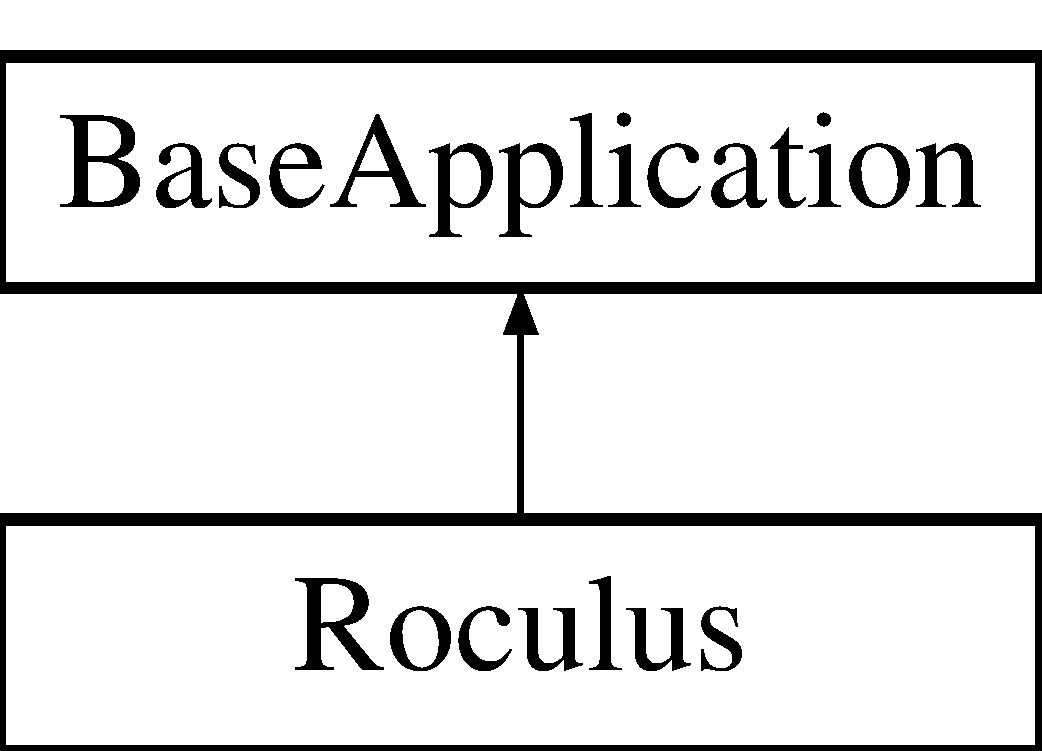
\includegraphics[height=2.000000cm]{classRoculus}
\end{center}
\end{figure}
\subsection*{\-Public \-Member \-Functions}
\begin{DoxyCompactItemize}
\item 
\hyperlink{classRoculus_a73729ed3b3134557e18df7b67b4171c5}{\-Roculus} (void)
\item 
virtual \hyperlink{classRoculus_aa839f9c21064f6a6f59e1a6e60afdef9}{$\sim$\-Roculus} (void)
\end{DoxyCompactItemize}
\subsection*{\-Protected \-Member \-Functions}
\begin{DoxyCompactItemize}
\item 
virtual void \hyperlink{classRoculus_a2da8d57d448a37e544d86d51e610f9d6}{create\-Scene} (void)
\item 
virtual void \hyperlink{classRoculus_a47dc1fd07bd9cd79b2f4cb8b95e53a5a}{load\-Recorded\-Scene} ()
\end{DoxyCompactItemize}


\subsection{\-Detailed \-Description}
class to take care of the scene and object creation. \-This class fills the scene with objects and in most cases creates the geometries manually. \-It has a method to parse room recordings in folders in order to include them into the scene. \-Though it is the nominal main class, the majority of the implementation is found in the \hyperlink{classBaseApplication}{\-Base\-Application} class. 

\subsection{\-Constructor \& \-Destructor \-Documentation}
\hypertarget{classRoculus_a73729ed3b3134557e18df7b67b4171c5}{\index{\-Roculus@{\-Roculus}!\-Roculus@{\-Roculus}}
\index{\-Roculus@{\-Roculus}!Roculus@{\-Roculus}}
\subsubsection[{\-Roculus}]{\setlength{\rightskip}{0pt plus 5cm}{\bf \-Roculus\-::\-Roculus} (
\begin{DoxyParamCaption}
\item[{void}]{}
\end{DoxyParamCaption}
)}}\label{classRoculus_a73729ed3b3134557e18df7b67b4171c5}
\-Default constructor \hypertarget{classRoculus_aa839f9c21064f6a6f59e1a6e60afdef9}{\index{\-Roculus@{\-Roculus}!$\sim$\-Roculus@{$\sim$\-Roculus}}
\index{$\sim$\-Roculus@{$\sim$\-Roculus}!Roculus@{\-Roculus}}
\subsubsection[{$\sim$\-Roculus}]{\setlength{\rightskip}{0pt plus 5cm}virtual {\bf \-Roculus\-::$\sim$\-Roculus} (
\begin{DoxyParamCaption}
\item[{void}]{}
\end{DoxyParamCaption}
)\hspace{0.3cm}{\ttfamily  \mbox{[}virtual\mbox{]}}}}\label{classRoculus_aa839f9c21064f6a6f59e1a6e60afdef9}
\-Default destructor 

\subsection{\-Member \-Function \-Documentation}
\hypertarget{classRoculus_a2da8d57d448a37e544d86d51e610f9d6}{\index{\-Roculus@{\-Roculus}!create\-Scene@{create\-Scene}}
\index{create\-Scene@{create\-Scene}!Roculus@{\-Roculus}}
\subsubsection[{create\-Scene}]{\setlength{\rightskip}{0pt plus 5cm}virtual void {\bf \-Roculus\-::create\-Scene} (
\begin{DoxyParamCaption}
\item[{void}]{}
\end{DoxyParamCaption}
)\hspace{0.3cm}{\ttfamily  \mbox{[}protected, virtual\mbox{]}}}}\label{classRoculus_a2da8d57d448a37e544d86d51e610f9d6}
\-Does the main work to compile the implemented manual objects into geometries (meshes) and to configure the materials and set up the \-Snapshot\-Libraries. \-N\-O\-T\-E\-: \-Includes hardcoded camera parameters for the standard geometry. 

\-Implements \hyperlink{classBaseApplication_aa97beeb4059b17d0ec22eae33286ec2d}{\-Base\-Application}.

\hypertarget{classRoculus_a47dc1fd07bd9cd79b2f4cb8b95e53a5a}{\index{\-Roculus@{\-Roculus}!load\-Recorded\-Scene@{load\-Recorded\-Scene}}
\index{load\-Recorded\-Scene@{load\-Recorded\-Scene}!Roculus@{\-Roculus}}
\subsubsection[{load\-Recorded\-Scene}]{\setlength{\rightskip}{0pt plus 5cm}virtual void {\bf \-Roculus\-::load\-Recorded\-Scene} (
\begin{DoxyParamCaption}
{}
\end{DoxyParamCaption}
)\hspace{0.3cm}{\ttfamily  \mbox{[}protected, virtual\mbox{]}}}}\label{classRoculus_a47dc1fd07bd9cd79b2f4cb8b95e53a5a}
\-Hardcodes the './map/' directory to be searched for room recordings and load them into a \hyperlink{classSnapshotLibrary}{\-Snapshot\-Library}. \-Includes smoothing for the depth images. 

\-The documentation for this class was generated from the following file\-:\begin{DoxyCompactItemize}
\item 
roculus/include/\-Roculus.\-h\end{DoxyCompactItemize}

\hypertarget{classRoom}{\section{\-Room \-Class \-Reference}
\label{classRoom}\index{\-Room@{\-Room}}
}


\-Describes a \hyperlink{classRoom}{\-Room} in a \hyperlink{classGame}{\-Game}. \-This class collects all parameters for a \hyperlink{classRoom}{\-Room}. \-It keeps track of the corresponding \-Way\-Points, \hyperlink{classDoor}{\-Door} nodes and event nodes and provides some utility functions.  




{\ttfamily \#include $<$\-Room.\-h$>$}

\subsection*{\-Public \-Member \-Functions}
\begin{DoxyCompactItemize}
\item 
\hyperlink{classRoom_aeca494ef2b98b46ab80620ddda354bdb}{\-Room} (int)
\item 
std\-::vector$<$ \hyperlink{classWayPoint}{\-Way\-Point} $\ast$ $>$ \& \hyperlink{classRoom_a8ada2aba11643989125c52056f21fdfb}{get\-W\-Ps} ()
\item 
std\-::vector$<$ \hyperlink{classWayPoint}{\-Way\-Point} $\ast$ $>$ \& \hyperlink{classRoom_a969be8dbe4444e7be92b4107337c8109}{get\-W\-Ps2\-Use} ()
\item 
bool \hyperlink{classRoom_adc25ce4a3d509baf2d74ce4feaadcfbd}{is\-Locked} ()
\item 
void \hyperlink{classRoom_a90ca4dec3d3040ac2ab9558da6bd024a}{lock} ()
\item 
void \hyperlink{classRoom_a58285cba499484ecbbdba37e81b7205f}{unlock} ()
\item 
int \hyperlink{classRoom_a2d9554ac5bb8f261fd38238eab0e6f02}{get\-Room\-Id} ()
\item 
\hyperlink{classWayPoint}{\-Way\-Point} $\ast$ \hyperlink{classRoom_a289489d94ab8471aa9213e57f31fdbfd}{get\-Door\-Evt} ()
\item 
\hyperlink{classWayPoint}{\-Way\-Point} $\ast$ \hyperlink{classRoom_a2a5c4f4ebb5fab1f30c7ef2507352269}{get\-Door\-W\-P} ()
\item 
void \hyperlink{classRoom_af7a4019ac279db263ac1aaa3daeb6452}{set\-Door\-Evt} (\hyperlink{classWayPoint}{\-Way\-Point} $\ast$)
\item 
void \hyperlink{classRoom_a0969d7fef8ee5df46f4f7f092356e727}{add\-Room\-Point} (\hyperlink{classWayPoint}{\-Way\-Point} $\ast$)
\item 
void \hyperlink{classRoom_add8ba3c88fb1d25e5e7ef45871de33d1}{add\-Use\-Point} (\hyperlink{classWayPoint}{\-Way\-Point} $\ast$)
\item 
void \hyperlink{classRoom_a1a07570c9de0f1830b54378daea77107}{set\-Door} (\hyperlink{classWayPoint}{\-Way\-Point} $\ast$)
\item 
void \hyperlink{classRoom_a8d4ac41b692d89e589b695b53b8cb8f6}{print} ()
\end{DoxyCompactItemize}
\subsection*{\-Protected \-Attributes}
\begin{DoxyCompactItemize}
\item 
int \hyperlink{classRoom_af51865ded79b022a93c6af4bd613d41c}{id}
\item 
std\-::vector$<$ \hyperlink{classWayPoint}{\-Way\-Point} $\ast$ $>$ \hyperlink{classRoom_a672a853c876de647aec33a2ad4da0471}{room\-Points}
\item 
bool \hyperlink{classRoom_a7d1c69d12f2fe191ad142be4fec461d4}{locked}
\item 
\hyperlink{classWayPoint}{\-Way\-Point} $\ast$ \hyperlink{classRoom_a44fa43dc49bfee1a50fa7c39075bf1cb}{door}
\item 
\hyperlink{classWayPoint}{\-Way\-Point} $\ast$ \hyperlink{classRoom_ab39232499fc239f45e16c26226ca842e}{door\-Event\-W\-P}
\item 
std\-::vector$<$ \hyperlink{classWayPoint}{\-Way\-Point} $\ast$ $>$ \hyperlink{classRoom_a56e6a07d53a2514d7538b72f56bcbf45}{use\-Points}
\end{DoxyCompactItemize}


\subsection{\-Detailed \-Description}
\-Describes a \hyperlink{classRoom}{\-Room} in a \hyperlink{classGame}{\-Game}. \-This class collects all parameters for a \hyperlink{classRoom}{\-Room}. \-It keeps track of the corresponding \-Way\-Points, \hyperlink{classDoor}{\-Door} nodes and event nodes and provides some utility functions. 

$<$ 

\subsection{\-Constructor \& \-Destructor \-Documentation}
\hypertarget{classRoom_aeca494ef2b98b46ab80620ddda354bdb}{\index{\-Room@{\-Room}!\-Room@{\-Room}}
\index{\-Room@{\-Room}!Room@{\-Room}}
\subsubsection[{\-Room}]{\setlength{\rightskip}{0pt plus 5cm}{\bf \-Room\-::\-Room} (
\begin{DoxyParamCaption}
\item[{int}]{}
\end{DoxyParamCaption}
)}}\label{classRoom_aeca494ef2b98b46ab80620ddda354bdb}
\-Initialize the room, assigning its \-I\-D. 

\subsection{\-Member \-Function \-Documentation}
\hypertarget{classRoom_a0969d7fef8ee5df46f4f7f092356e727}{\index{\-Room@{\-Room}!add\-Room\-Point@{add\-Room\-Point}}
\index{add\-Room\-Point@{add\-Room\-Point}!Room@{\-Room}}
\subsubsection[{add\-Room\-Point}]{\setlength{\rightskip}{0pt plus 5cm}void {\bf \-Room\-::add\-Room\-Point} (
\begin{DoxyParamCaption}
\item[{{\bf \-Way\-Point} $\ast$}]{}
\end{DoxyParamCaption}
)}}\label{classRoom_a0969d7fef8ee5df46f4f7f092356e727}
\-Add a \hyperlink{classWayPoint}{\-Way\-Point} to the room. \hypertarget{classRoom_add8ba3c88fb1d25e5e7ef45871de33d1}{\index{\-Room@{\-Room}!add\-Use\-Point@{add\-Use\-Point}}
\index{add\-Use\-Point@{add\-Use\-Point}!Room@{\-Room}}
\subsubsection[{add\-Use\-Point}]{\setlength{\rightskip}{0pt plus 5cm}void {\bf \-Room\-::add\-Use\-Point} (
\begin{DoxyParamCaption}
\item[{{\bf \-Way\-Point} $\ast$}]{}
\end{DoxyParamCaption}
)}}\label{classRoom_add8ba3c88fb1d25e5e7ef45871de33d1}
\-Add a \hyperlink{classWayPoint}{\-Way\-Point} to the set of \-Way\-Points to use for \-Keys/\-Treasures. \hypertarget{classRoom_a289489d94ab8471aa9213e57f31fdbfd}{\index{\-Room@{\-Room}!get\-Door\-Evt@{get\-Door\-Evt}}
\index{get\-Door\-Evt@{get\-Door\-Evt}!Room@{\-Room}}
\subsubsection[{get\-Door\-Evt}]{\setlength{\rightskip}{0pt plus 5cm}{\bf \-Way\-Point}$\ast$ {\bf \-Room\-::get\-Door\-Evt} (
\begin{DoxyParamCaption}
{}
\end{DoxyParamCaption}
)}}\label{classRoom_a289489d94ab8471aa9213e57f31fdbfd}
\-Returns the \hyperlink{classWayPoint}{\-Way\-Point} which triggers the door event. \hypertarget{classRoom_a2a5c4f4ebb5fab1f30c7ef2507352269}{\index{\-Room@{\-Room}!get\-Door\-W\-P@{get\-Door\-W\-P}}
\index{get\-Door\-W\-P@{get\-Door\-W\-P}!Room@{\-Room}}
\subsubsection[{get\-Door\-W\-P}]{\setlength{\rightskip}{0pt plus 5cm}{\bf \-Way\-Point}$\ast$ {\bf \-Room\-::get\-Door\-W\-P} (
\begin{DoxyParamCaption}
{}
\end{DoxyParamCaption}
)}}\label{classRoom_a2a5c4f4ebb5fab1f30c7ef2507352269}
\-Returns the \hyperlink{classWayPoint}{\-Way\-Point} which denotes the door. \-In fact the door will be placed half way between the door\-W\-P and the door\-Event\-W\-P. \hypertarget{classRoom_a2d9554ac5bb8f261fd38238eab0e6f02}{\index{\-Room@{\-Room}!get\-Room\-Id@{get\-Room\-Id}}
\index{get\-Room\-Id@{get\-Room\-Id}!Room@{\-Room}}
\subsubsection[{get\-Room\-Id}]{\setlength{\rightskip}{0pt plus 5cm}int {\bf \-Room\-::get\-Room\-Id} (
\begin{DoxyParamCaption}
{}
\end{DoxyParamCaption}
)}}\label{classRoom_a2d9554ac5bb8f261fd38238eab0e6f02}
\-Returns the \-I\-D of this room. \hypertarget{classRoom_a8ada2aba11643989125c52056f21fdfb}{\index{\-Room@{\-Room}!get\-W\-Ps@{get\-W\-Ps}}
\index{get\-W\-Ps@{get\-W\-Ps}!Room@{\-Room}}
\subsubsection[{get\-W\-Ps}]{\setlength{\rightskip}{0pt plus 5cm}std\-::vector$<${\bf \-Way\-Point}$\ast$$>$\& {\bf \-Room\-::get\-W\-Ps} (
\begin{DoxyParamCaption}
{}
\end{DoxyParamCaption}
)}}\label{classRoom_a8ada2aba11643989125c52056f21fdfb}
\-Returns the vector of all \-Way\-Points that are in this room. \hypertarget{classRoom_a969be8dbe4444e7be92b4107337c8109}{\index{\-Room@{\-Room}!get\-W\-Ps2\-Use@{get\-W\-Ps2\-Use}}
\index{get\-W\-Ps2\-Use@{get\-W\-Ps2\-Use}!Room@{\-Room}}
\subsubsection[{get\-W\-Ps2\-Use}]{\setlength{\rightskip}{0pt plus 5cm}std\-::vector$<${\bf \-Way\-Point}$\ast$$>$\& {\bf \-Room\-::get\-W\-Ps2\-Use} (
\begin{DoxyParamCaption}
{}
\end{DoxyParamCaption}
)}}\label{classRoom_a969be8dbe4444e7be92b4107337c8109}
\-Returns the vector of \-Way\-Points that can be used to place \-Keys/\-Treasures. \hypertarget{classRoom_adc25ce4a3d509baf2d74ce4feaadcfbd}{\index{\-Room@{\-Room}!is\-Locked@{is\-Locked}}
\index{is\-Locked@{is\-Locked}!Room@{\-Room}}
\subsubsection[{is\-Locked}]{\setlength{\rightskip}{0pt plus 5cm}bool {\bf \-Room\-::is\-Locked} (
\begin{DoxyParamCaption}
{}
\end{DoxyParamCaption}
)}}\label{classRoom_adc25ce4a3d509baf2d74ce4feaadcfbd}
\-Is this room locked? \hypertarget{classRoom_a90ca4dec3d3040ac2ab9558da6bd024a}{\index{\-Room@{\-Room}!lock@{lock}}
\index{lock@{lock}!Room@{\-Room}}
\subsubsection[{lock}]{\setlength{\rightskip}{0pt plus 5cm}void {\bf \-Room\-::lock} (
\begin{DoxyParamCaption}
{}
\end{DoxyParamCaption}
)}}\label{classRoom_a90ca4dec3d3040ac2ab9558da6bd024a}
\hyperlink{classLock}{\-Lock} this room\-: make its \-Way\-Points unavailable for selection. \hypertarget{classRoom_a8d4ac41b692d89e589b695b53b8cb8f6}{\index{\-Room@{\-Room}!print@{print}}
\index{print@{print}!Room@{\-Room}}
\subsubsection[{print}]{\setlength{\rightskip}{0pt plus 5cm}void {\bf \-Room\-::print} (
\begin{DoxyParamCaption}
{}
\end{DoxyParamCaption}
)}}\label{classRoom_a8d4ac41b692d89e589b695b53b8cb8f6}
\-Utility function. \-Print the room configuration on the console. \-Useful for debugging. \hypertarget{classRoom_a1a07570c9de0f1830b54378daea77107}{\index{\-Room@{\-Room}!set\-Door@{set\-Door}}
\index{set\-Door@{set\-Door}!Room@{\-Room}}
\subsubsection[{set\-Door}]{\setlength{\rightskip}{0pt plus 5cm}void {\bf \-Room\-::set\-Door} (
\begin{DoxyParamCaption}
\item[{{\bf \-Way\-Point} $\ast$}]{}
\end{DoxyParamCaption}
)}}\label{classRoom_a1a07570c9de0f1830b54378daea77107}
\-Set the \hyperlink{classWayPoint}{\-Way\-Point} which denotes the door. \hypertarget{classRoom_af7a4019ac279db263ac1aaa3daeb6452}{\index{\-Room@{\-Room}!set\-Door\-Evt@{set\-Door\-Evt}}
\index{set\-Door\-Evt@{set\-Door\-Evt}!Room@{\-Room}}
\subsubsection[{set\-Door\-Evt}]{\setlength{\rightskip}{0pt plus 5cm}void {\bf \-Room\-::set\-Door\-Evt} (
\begin{DoxyParamCaption}
\item[{{\bf \-Way\-Point} $\ast$}]{}
\end{DoxyParamCaption}
)}}\label{classRoom_af7a4019ac279db263ac1aaa3daeb6452}
\-Set the \hyperlink{classWayPoint}{\-Way\-Point} which triggers the door event. \hypertarget{classRoom_a58285cba499484ecbbdba37e81b7205f}{\index{\-Room@{\-Room}!unlock@{unlock}}
\index{unlock@{unlock}!Room@{\-Room}}
\subsubsection[{unlock}]{\setlength{\rightskip}{0pt plus 5cm}void {\bf \-Room\-::unlock} (
\begin{DoxyParamCaption}
{}
\end{DoxyParamCaption}
)}}\label{classRoom_a58285cba499484ecbbdba37e81b7205f}
\-Unlock the room\-: make its \-Way\-Points accessible again. 

\subsection{\-Member \-Data \-Documentation}
\hypertarget{classRoom_a44fa43dc49bfee1a50fa7c39075bf1cb}{\index{\-Room@{\-Room}!door@{door}}
\index{door@{door}!Room@{\-Room}}
\subsubsection[{door}]{\setlength{\rightskip}{0pt plus 5cm}{\bf \-Way\-Point}$\ast$ {\bf \-Room\-::door}\hspace{0.3cm}{\ttfamily  \mbox{[}protected\mbox{]}}}}\label{classRoom_a44fa43dc49bfee1a50fa7c39075bf1cb}
\-In case this room will be used as \hyperlink{classTreasure}{\-Treasure} chamber, which \hyperlink{classWayPoint}{\-Way\-Point} marks the \hyperlink{classDoor}{\-Door}? \hypertarget{classRoom_ab39232499fc239f45e16c26226ca842e}{\index{\-Room@{\-Room}!door\-Event\-W\-P@{door\-Event\-W\-P}}
\index{door\-Event\-W\-P@{door\-Event\-W\-P}!Room@{\-Room}}
\subsubsection[{door\-Event\-W\-P}]{\setlength{\rightskip}{0pt plus 5cm}{\bf \-Way\-Point}$\ast$ {\bf \-Room\-::door\-Event\-W\-P}\hspace{0.3cm}{\ttfamily  \mbox{[}protected\mbox{]}}}}\label{classRoom_ab39232499fc239f45e16c26226ca842e}
\-In case this room will be used as \hyperlink{classTreasure}{\-Treasure} chamber, which \hyperlink{classWayPoint}{\-Way\-Point} triggers the \hyperlink{classDoor}{\-Door} event? \hypertarget{classRoom_af51865ded79b022a93c6af4bd613d41c}{\index{\-Room@{\-Room}!id@{id}}
\index{id@{id}!Room@{\-Room}}
\subsubsection[{id}]{\setlength{\rightskip}{0pt plus 5cm}int {\bf \-Room\-::id}\hspace{0.3cm}{\ttfamily  \mbox{[}protected\mbox{]}}}}\label{classRoom_af51865ded79b022a93c6af4bd613d41c}
\-The number/\-I\-D of this room. \hypertarget{classRoom_a7d1c69d12f2fe191ad142be4fec461d4}{\index{\-Room@{\-Room}!locked@{locked}}
\index{locked@{locked}!Room@{\-Room}}
\subsubsection[{locked}]{\setlength{\rightskip}{0pt plus 5cm}bool {\bf \-Room\-::locked}\hspace{0.3cm}{\ttfamily  \mbox{[}protected\mbox{]}}}}\label{classRoom_a7d1c69d12f2fe191ad142be4fec461d4}
\-Stores if the room is locked. \hypertarget{classRoom_a672a853c876de647aec33a2ad4da0471}{\index{\-Room@{\-Room}!room\-Points@{room\-Points}}
\index{room\-Points@{room\-Points}!Room@{\-Room}}
\subsubsection[{room\-Points}]{\setlength{\rightskip}{0pt plus 5cm}std\-::vector$<${\bf \-Way\-Point}$\ast$$>$ {\bf \-Room\-::room\-Points}\hspace{0.3cm}{\ttfamily  \mbox{[}protected\mbox{]}}}}\label{classRoom_a672a853c876de647aec33a2ad4da0471}
\-All \-Way\-Points that belong to this room. \hypertarget{classRoom_a56e6a07d53a2514d7538b72f56bcbf45}{\index{\-Room@{\-Room}!use\-Points@{use\-Points}}
\index{use\-Points@{use\-Points}!Room@{\-Room}}
\subsubsection[{use\-Points}]{\setlength{\rightskip}{0pt plus 5cm}std\-::vector$<${\bf \-Way\-Point}$\ast$$>$ {\bf \-Room\-::use\-Points}\hspace{0.3cm}{\ttfamily  \mbox{[}protected\mbox{]}}}}\label{classRoom_a56e6a07d53a2514d7538b72f56bcbf45}
\-Which \-Way\-Points can be used to place \-Keys or the \hyperlink{classTreasure}{\-Treasure}? 

\-The documentation for this class was generated from the following file\-:\begin{DoxyCompactItemize}
\item 
roculus/include/\-Room.\-h\end{DoxyCompactItemize}

\hypertarget{classSnapshot}{\section{\-Snapshot \-Class \-Reference}
\label{classSnapshot}\index{\-Snapshot@{\-Snapshot}}
}


\-Collects all data that describes a \hyperlink{classSnapshot}{\-Snapshot} and provides a method to insert it into the scene. (\-Not the smartest implementation, should probably be constructed given the scene manager and do the object creation by itself. \-Static counter would help to identify total number of \-Snapshots to link to individual materials, textures etc.)  




{\ttfamily \#include $<$\-Snapshot.\-h$>$}

\subsection*{\-Public \-Member \-Functions}
\begin{DoxyCompactItemize}
\item 
\hyperlink{classSnapshot_ac23b92a6b8dba7231deb0eabe380f7f4}{\-Snapshot} (\-Ogre\-::\-Entity $\ast$, \-Ogre\-::\-Scene\-Node $\ast$, const \-Ogre\-::\-Texture\-Ptr \&, const \-Ogre\-::\-Texture\-Ptr \&)
\item 
\hyperlink{classSnapshot_ac9793a7337c8b514c7679eb0a82b9328}{$\sim$\-Snapshot} ()
\item 
virtual \-Ogre\-::\-Scene\-Node $\ast$ \hyperlink{classSnapshot_ade78092b22032565fd191442be26106e}{get\-Target\-Scene\-Node} ()
\item 
virtual \-Ogre\-::\-Texture\-Ptr \hyperlink{classSnapshot_a2d025a7e4000ea6da3333d5f85127b14}{get\-Assigned\-Depth\-Texture} ()
\item 
virtual \-Ogre\-::\-Texture\-Ptr \hyperlink{classSnapshot_aec0736e686c5fb103dc4e0e4133c1df0}{get\-Assigned\-R\-G\-B\-Texture} ()
\item 
virtual void \hyperlink{classSnapshot_afa35ce833d0b5668eb04436bd581f2c0}{set\-Target\-Scene\-Node} (\-Ogre\-::\-Scene\-Node $\ast$)
\item 
virtual void \hyperlink{classSnapshot_ae21564f3fe2cc65bba44d25bb691ffb5}{assign\-Depth\-Texture} (const \-Ogre\-::\-Texture\-Ptr \&)
\item 
virtual void \hyperlink{classSnapshot_a55c7abcd9c234bb0fe9a0dc22786fdae}{assign\-R\-G\-B\-Texture} (const \-Ogre\-::\-Texture\-Ptr \&)
\item 
virtual bool \hyperlink{classSnapshot_ad3c7ad06b61678ded3dd022aab511ec4}{place\-In\-Scene} (const \-Ogre\-::\-Image \&, const \-Ogre\-::\-Image \&, const \-Ogre\-::\-Vector3 \&, const \-Ogre\-::\-Quaternion \&)
\end{DoxyCompactItemize}
\subsection*{\-Protected \-Attributes}
\begin{DoxyCompactItemize}
\item 
\-Ogre\-::\-Entity $\ast$ \hyperlink{classSnapshot_a049a4347e562c85029ddc099dc019e17}{snapshot}
\item 
\-Ogre\-::\-Texture\-Ptr \hyperlink{classSnapshot_aa568adf9051f6eb80353f7f1673cdb33}{depth\-Texture}
\item 
\-Ogre\-::\-Texture\-Ptr \hyperlink{classSnapshot_af759834693d9319f38be4e3d3cbe48c0}{rgb\-Texture}
\item 
\-Ogre\-::\-Scene\-Node $\ast$ \hyperlink{classSnapshot_ab86c0038377f46c94957bf5634c74b03}{target\-Scene\-Node}
\item 
bool \hyperlink{classSnapshot_a0c9100c6611542fafa58b9bcde75bc3d}{attached}
\end{DoxyCompactItemize}


\subsection{\-Detailed \-Description}
\-Collects all data that describes a \hyperlink{classSnapshot}{\-Snapshot} and provides a method to insert it into the scene. (\-Not the smartest implementation, should probably be constructed given the scene manager and do the object creation by itself. \-Static counter would help to identify total number of \-Snapshots to link to individual materials, textures etc.) 

\subsection{\-Constructor \& \-Destructor \-Documentation}
\hypertarget{classSnapshot_ac23b92a6b8dba7231deb0eabe380f7f4}{\index{\-Snapshot@{\-Snapshot}!\-Snapshot@{\-Snapshot}}
\index{\-Snapshot@{\-Snapshot}!Snapshot@{\-Snapshot}}
\subsubsection[{\-Snapshot}]{\setlength{\rightskip}{0pt plus 5cm}{\bf \-Snapshot\-::\-Snapshot} (
\begin{DoxyParamCaption}
\item[{\-Ogre\-::\-Entity $\ast$}]{, }
\item[{\-Ogre\-::\-Scene\-Node $\ast$}]{, }
\item[{const \-Ogre\-::\-Texture\-Ptr \&}]{, }
\item[{const \-Ogre\-::\-Texture\-Ptr \&}]{}
\end{DoxyParamCaption}
)}}\label{classSnapshot_ac23b92a6b8dba7231deb0eabe380f7f4}
\-Initializes this object with an \-Ogre\-::\-Entity (an instance of the camera geometry), a \-Scene\-Node (on which the object is placed), and two texture pointers for the depth-\/information (first pointer) and the rgb-\/information (second pointer). \hypertarget{classSnapshot_ac9793a7337c8b514c7679eb0a82b9328}{\index{\-Snapshot@{\-Snapshot}!$\sim$\-Snapshot@{$\sim$\-Snapshot}}
\index{$\sim$\-Snapshot@{$\sim$\-Snapshot}!Snapshot@{\-Snapshot}}
\subsubsection[{$\sim$\-Snapshot}]{\setlength{\rightskip}{0pt plus 5cm}{\bf \-Snapshot\-::$\sim$\-Snapshot} (
\begin{DoxyParamCaption}
{}
\end{DoxyParamCaption}
)}}\label{classSnapshot_ac9793a7337c8b514c7679eb0a82b9328}
\-Default destructor. 

\subsection{\-Member \-Function \-Documentation}
\hypertarget{classSnapshot_ae21564f3fe2cc65bba44d25bb691ffb5}{\index{\-Snapshot@{\-Snapshot}!assign\-Depth\-Texture@{assign\-Depth\-Texture}}
\index{assign\-Depth\-Texture@{assign\-Depth\-Texture}!Snapshot@{\-Snapshot}}
\subsubsection[{assign\-Depth\-Texture}]{\setlength{\rightskip}{0pt plus 5cm}virtual void {\bf \-Snapshot\-::assign\-Depth\-Texture} (
\begin{DoxyParamCaption}
\item[{const \-Ogre\-::\-Texture\-Ptr \&}]{}
\end{DoxyParamCaption}
)\hspace{0.3cm}{\ttfamily  \mbox{[}virtual\mbox{]}}}}\label{classSnapshot_ae21564f3fe2cc65bba44d25bb691ffb5}
\-Assign a depth-\/texture to the snapshot. \hypertarget{classSnapshot_a55c7abcd9c234bb0fe9a0dc22786fdae}{\index{\-Snapshot@{\-Snapshot}!assign\-R\-G\-B\-Texture@{assign\-R\-G\-B\-Texture}}
\index{assign\-R\-G\-B\-Texture@{assign\-R\-G\-B\-Texture}!Snapshot@{\-Snapshot}}
\subsubsection[{assign\-R\-G\-B\-Texture}]{\setlength{\rightskip}{0pt plus 5cm}virtual void {\bf \-Snapshot\-::assign\-R\-G\-B\-Texture} (
\begin{DoxyParamCaption}
\item[{const \-Ogre\-::\-Texture\-Ptr \&}]{}
\end{DoxyParamCaption}
)\hspace{0.3cm}{\ttfamily  \mbox{[}virtual\mbox{]}}}}\label{classSnapshot_a55c7abcd9c234bb0fe9a0dc22786fdae}
\-Assign a rgb-\/texture to the snapshot. \hypertarget{classSnapshot_a2d025a7e4000ea6da3333d5f85127b14}{\index{\-Snapshot@{\-Snapshot}!get\-Assigned\-Depth\-Texture@{get\-Assigned\-Depth\-Texture}}
\index{get\-Assigned\-Depth\-Texture@{get\-Assigned\-Depth\-Texture}!Snapshot@{\-Snapshot}}
\subsubsection[{get\-Assigned\-Depth\-Texture}]{\setlength{\rightskip}{0pt plus 5cm}virtual \-Ogre\-::\-Texture\-Ptr {\bf \-Snapshot\-::get\-Assigned\-Depth\-Texture} (
\begin{DoxyParamCaption}
{}
\end{DoxyParamCaption}
)\hspace{0.3cm}{\ttfamily  \mbox{[}virtual\mbox{]}}}}\label{classSnapshot_a2d025a7e4000ea6da3333d5f85127b14}
\-Returns the depth-\/texture pointer for this snapshot. \hypertarget{classSnapshot_aec0736e686c5fb103dc4e0e4133c1df0}{\index{\-Snapshot@{\-Snapshot}!get\-Assigned\-R\-G\-B\-Texture@{get\-Assigned\-R\-G\-B\-Texture}}
\index{get\-Assigned\-R\-G\-B\-Texture@{get\-Assigned\-R\-G\-B\-Texture}!Snapshot@{\-Snapshot}}
\subsubsection[{get\-Assigned\-R\-G\-B\-Texture}]{\setlength{\rightskip}{0pt plus 5cm}virtual \-Ogre\-::\-Texture\-Ptr {\bf \-Snapshot\-::get\-Assigned\-R\-G\-B\-Texture} (
\begin{DoxyParamCaption}
{}
\end{DoxyParamCaption}
)\hspace{0.3cm}{\ttfamily  \mbox{[}virtual\mbox{]}}}}\label{classSnapshot_aec0736e686c5fb103dc4e0e4133c1df0}
\-Returns the rgb-\/texture pointer for this snapshot. \hypertarget{classSnapshot_ade78092b22032565fd191442be26106e}{\index{\-Snapshot@{\-Snapshot}!get\-Target\-Scene\-Node@{get\-Target\-Scene\-Node}}
\index{get\-Target\-Scene\-Node@{get\-Target\-Scene\-Node}!Snapshot@{\-Snapshot}}
\subsubsection[{get\-Target\-Scene\-Node}]{\setlength{\rightskip}{0pt plus 5cm}virtual \-Ogre\-::\-Scene\-Node$\ast$ {\bf \-Snapshot\-::get\-Target\-Scene\-Node} (
\begin{DoxyParamCaption}
{}
\end{DoxyParamCaption}
)\hspace{0.3cm}{\ttfamily  \mbox{[}virtual\mbox{]}}}}\label{classSnapshot_ade78092b22032565fd191442be26106e}
\-Returns the scene node of this object. \hypertarget{classSnapshot_ad3c7ad06b61678ded3dd022aab511ec4}{\index{\-Snapshot@{\-Snapshot}!place\-In\-Scene@{place\-In\-Scene}}
\index{place\-In\-Scene@{place\-In\-Scene}!Snapshot@{\-Snapshot}}
\subsubsection[{place\-In\-Scene}]{\setlength{\rightskip}{0pt plus 5cm}virtual bool {\bf \-Snapshot\-::place\-In\-Scene} (
\begin{DoxyParamCaption}
\item[{const \-Ogre\-::\-Image \&}]{, }
\item[{const \-Ogre\-::\-Image \&}]{, }
\item[{const \-Ogre\-::\-Vector3 \&}]{, }
\item[{const \-Ogre\-::\-Quaternion \&}]{}
\end{DoxyParamCaption}
)\hspace{0.3cm}{\ttfamily  \mbox{[}virtual\mbox{]}}}}\label{classSnapshot_ad3c7ad06b61678ded3dd022aab511ec4}
\-Given a depth image (1st), a rgb image (2nd), the corresponding camera position and orientation, place a snapshot in the scene. \hypertarget{classSnapshot_afa35ce833d0b5668eb04436bd581f2c0}{\index{\-Snapshot@{\-Snapshot}!set\-Target\-Scene\-Node@{set\-Target\-Scene\-Node}}
\index{set\-Target\-Scene\-Node@{set\-Target\-Scene\-Node}!Snapshot@{\-Snapshot}}
\subsubsection[{set\-Target\-Scene\-Node}]{\setlength{\rightskip}{0pt plus 5cm}virtual void {\bf \-Snapshot\-::set\-Target\-Scene\-Node} (
\begin{DoxyParamCaption}
\item[{\-Ogre\-::\-Scene\-Node $\ast$}]{}
\end{DoxyParamCaption}
)\hspace{0.3cm}{\ttfamily  \mbox{[}virtual\mbox{]}}}}\label{classSnapshot_afa35ce833d0b5668eb04436bd581f2c0}
\-Sets the scene node for this object. (\-Not used currently -\/ \-D\-E\-P\-R\-E\-C\-A\-T\-E\-D). 

\subsection{\-Member \-Data \-Documentation}
\hypertarget{classSnapshot_a0c9100c6611542fafa58b9bcde75bc3d}{\index{\-Snapshot@{\-Snapshot}!attached@{attached}}
\index{attached@{attached}!Snapshot@{\-Snapshot}}
\subsubsection[{attached}]{\setlength{\rightskip}{0pt plus 5cm}bool {\bf \-Snapshot\-::attached}\hspace{0.3cm}{\ttfamily  \mbox{[}protected\mbox{]}}}}\label{classSnapshot_a0c9100c6611542fafa58b9bcde75bc3d}
\-Was this snapshot already attached to its scene node? (\-Needed in place\-In\-Scene(...)) \hypertarget{classSnapshot_aa568adf9051f6eb80353f7f1673cdb33}{\index{\-Snapshot@{\-Snapshot}!depth\-Texture@{depth\-Texture}}
\index{depth\-Texture@{depth\-Texture}!Snapshot@{\-Snapshot}}
\subsubsection[{depth\-Texture}]{\setlength{\rightskip}{0pt plus 5cm}\-Ogre\-::\-Texture\-Ptr {\bf \-Snapshot\-::depth\-Texture}\hspace{0.3cm}{\ttfamily  \mbox{[}protected\mbox{]}}}}\label{classSnapshot_aa568adf9051f6eb80353f7f1673cdb33}
\-Pointer to the depth texture for this snapshot. \hypertarget{classSnapshot_af759834693d9319f38be4e3d3cbe48c0}{\index{\-Snapshot@{\-Snapshot}!rgb\-Texture@{rgb\-Texture}}
\index{rgb\-Texture@{rgb\-Texture}!Snapshot@{\-Snapshot}}
\subsubsection[{rgb\-Texture}]{\setlength{\rightskip}{0pt plus 5cm}\-Ogre\-::\-Texture\-Ptr {\bf \-Snapshot\-::rgb\-Texture}\hspace{0.3cm}{\ttfamily  \mbox{[}protected\mbox{]}}}}\label{classSnapshot_af759834693d9319f38be4e3d3cbe48c0}
\-Pointer to the rgb texture for this snapshot. \hypertarget{classSnapshot_a049a4347e562c85029ddc099dc019e17}{\index{\-Snapshot@{\-Snapshot}!snapshot@{snapshot}}
\index{snapshot@{snapshot}!Snapshot@{\-Snapshot}}
\subsubsection[{snapshot}]{\setlength{\rightskip}{0pt plus 5cm}\-Ogre\-::\-Entity$\ast$ {\bf \-Snapshot\-::snapshot}\hspace{0.3cm}{\ttfamily  \mbox{[}protected\mbox{]}}}}\label{classSnapshot_a049a4347e562c85029ddc099dc019e17}
\-Ogre\-::\-Entity for this snapshot. (\-An instance of the camera geometry). \hypertarget{classSnapshot_ab86c0038377f46c94957bf5634c74b03}{\index{\-Snapshot@{\-Snapshot}!target\-Scene\-Node@{target\-Scene\-Node}}
\index{target\-Scene\-Node@{target\-Scene\-Node}!Snapshot@{\-Snapshot}}
\subsubsection[{target\-Scene\-Node}]{\setlength{\rightskip}{0pt plus 5cm}\-Ogre\-::\-Scene\-Node$\ast$ {\bf \-Snapshot\-::target\-Scene\-Node}\hspace{0.3cm}{\ttfamily  \mbox{[}protected\mbox{]}}}}\label{classSnapshot_ab86c0038377f46c94957bf5634c74b03}
\-This snapshot's scene node. 

\-The documentation for this class was generated from the following file\-:\begin{DoxyCompactItemize}
\item 
roculus/include/\-Snapshot.\-h\end{DoxyCompactItemize}

\hypertarget{classSnapshotLibrary}{\section{\-Snapshot\-Library \-Class \-Reference}
\label{classSnapshotLibrary}\index{\-Snapshot\-Library@{\-Snapshot\-Library}}
}


\-Groups multiple \-Snapshots in a library (vector). \-Furthermore, this class manages the memory and preallocates \-Ogre\-::\-Textures, \-Materials and \-Scene\-Nodes, whenever needed.  




{\ttfamily \#include $<$\-Snapshot\-Library.\-h$>$}

\subsection*{\-Public \-Member \-Functions}
\begin{DoxyCompactItemize}
\item 
bool \hyperlink{classSnapshotLibrary_a211bd4eb1b15c8ae8dda57ff953528e1}{place\-In\-Scene} (const \-Ogre\-::\-Image \&, const \-Ogre\-::\-Image \&, const \-Ogre\-::\-Vector3 \&, const \-Ogre\-::\-Quaternion \&)
\item 
void \hyperlink{classSnapshotLibrary_ac8c6b6aaee929d20cdbfc3df95c61998}{flip\-Visibility} ()
\item 
\hyperlink{classSnapshotLibrary_a2db1cb6e6550c677b9a609964b7a74cb}{\-Snapshot\-Library} (\-Ogre\-::\-Scene\-Manager $\ast$, const \-Ogre\-::\-String \&, const \-Ogre\-::\-String \&, int)
\item 
\hyperlink{classSnapshotLibrary_a0eb263c926c8607b8943550984915933}{$\sim$\-Snapshot\-Library} ()
\end{DoxyCompactItemize}
\subsection*{\-Protected \-Member \-Functions}
\begin{DoxyCompactItemize}
\item 
void \hyperlink{classSnapshotLibrary_af8b18edc145bf95a04f3c64659ce0904}{allocate} (int)
\end{DoxyCompactItemize}
\subsection*{\-Protected \-Attributes}
\begin{DoxyCompactItemize}
\item 
std\-::vector$<$ \hyperlink{classSnapshot}{\-Snapshot} $\ast$ $>$ \hyperlink{classSnapshotLibrary_adc6f783d638a9ff4744b16bfa66b8953}{library}
\item 
int \hyperlink{classSnapshotLibrary_ac57409313d63db08bf743da47c768781}{current\-Snapshot}
\item 
int \hyperlink{classSnapshotLibrary_a8d1f7abf98dbb1f9cb8e82657218b850}{max\-Snapshots}
\item 
\-Ogre\-::\-String \hyperlink{classSnapshotLibrary_a968263cf5e86e9d2be54bae17fd69b00}{\-Entity\-Prototype}
\item 
\-Ogre\-::\-String \hyperlink{classSnapshotLibrary_a34479d4ccada0297ff80a41a4adf5100}{\-Material\-Prototype}
\item 
\-Ogre\-::\-Scene\-Manager $\ast$ \hyperlink{classSnapshotLibrary_a59737af324c6e35b0fe67b1ad60b8a8a}{m\-Scene\-Mgr}
\item 
\-Ogre\-::\-Scene\-Node $\ast$ \hyperlink{classSnapshotLibrary_aa510467111273c06dceeb3435d586e66}{m\-Master\-Scene\-Node}
\end{DoxyCompactItemize}


\subsection{\-Detailed \-Description}
\-Groups multiple \-Snapshots in a library (vector). \-Furthermore, this class manages the memory and preallocates \-Ogre\-::\-Textures, \-Materials and \-Scene\-Nodes, whenever needed. 

$<$ 

\subsection{\-Constructor \& \-Destructor \-Documentation}
\hypertarget{classSnapshotLibrary_a2db1cb6e6550c677b9a609964b7a74cb}{\index{\-Snapshot\-Library@{\-Snapshot\-Library}!\-Snapshot\-Library@{\-Snapshot\-Library}}
\index{\-Snapshot\-Library@{\-Snapshot\-Library}!SnapshotLibrary@{\-Snapshot\-Library}}
\subsubsection[{\-Snapshot\-Library}]{\setlength{\rightskip}{0pt plus 5cm}{\bf \-Snapshot\-Library\-::\-Snapshot\-Library} (
\begin{DoxyParamCaption}
\item[{\-Ogre\-::\-Scene\-Manager $\ast$}]{, }
\item[{const \-Ogre\-::\-String \&}]{, }
\item[{const \-Ogre\-::\-String \&}]{, }
\item[{int}]{}
\end{DoxyParamCaption}
)}}\label{classSnapshotLibrary_a2db1cb6e6550c677b9a609964b7a74cb}
\-Initialize the object with\-: (1) the scene manager (for object creation), (2) the entity prototype for the camera geometry, (3) the default material and (4) the number of snapshots for which memory should be preallocated each time. \hypertarget{classSnapshotLibrary_a0eb263c926c8607b8943550984915933}{\index{\-Snapshot\-Library@{\-Snapshot\-Library}!$\sim$\-Snapshot\-Library@{$\sim$\-Snapshot\-Library}}
\index{$\sim$\-Snapshot\-Library@{$\sim$\-Snapshot\-Library}!SnapshotLibrary@{\-Snapshot\-Library}}
\subsubsection[{$\sim$\-Snapshot\-Library}]{\setlength{\rightskip}{0pt plus 5cm}{\bf \-Snapshot\-Library\-::$\sim$\-Snapshot\-Library} (
\begin{DoxyParamCaption}
{}
\end{DoxyParamCaption}
)}}\label{classSnapshotLibrary_a0eb263c926c8607b8943550984915933}
\-Default destructor. 

\subsection{\-Member \-Function \-Documentation}
\hypertarget{classSnapshotLibrary_af8b18edc145bf95a04f3c64659ce0904}{\index{\-Snapshot\-Library@{\-Snapshot\-Library}!allocate@{allocate}}
\index{allocate@{allocate}!SnapshotLibrary@{\-Snapshot\-Library}}
\subsubsection[{allocate}]{\setlength{\rightskip}{0pt plus 5cm}void {\bf \-Snapshot\-Library\-::allocate} (
\begin{DoxyParamCaption}
\item[{int}]{}
\end{DoxyParamCaption}
)\hspace{0.3cm}{\ttfamily  \mbox{[}protected\mbox{]}}}}\label{classSnapshotLibrary_af8b18edc145bf95a04f3c64659ce0904}
\-Utility method to allocate new memory for a number of snapshots. \hypertarget{classSnapshotLibrary_ac8c6b6aaee929d20cdbfc3df95c61998}{\index{\-Snapshot\-Library@{\-Snapshot\-Library}!flip\-Visibility@{flip\-Visibility}}
\index{flip\-Visibility@{flip\-Visibility}!SnapshotLibrary@{\-Snapshot\-Library}}
\subsubsection[{flip\-Visibility}]{\setlength{\rightskip}{0pt plus 5cm}void {\bf \-Snapshot\-Library\-::flip\-Visibility} (
\begin{DoxyParamCaption}
{}
\end{DoxyParamCaption}
)}}\label{classSnapshotLibrary_ac8c6b6aaee929d20cdbfc3df95c61998}
\-Toggle the visiblity of all snapshots in the library. \hypertarget{classSnapshotLibrary_a211bd4eb1b15c8ae8dda57ff953528e1}{\index{\-Snapshot\-Library@{\-Snapshot\-Library}!place\-In\-Scene@{place\-In\-Scene}}
\index{place\-In\-Scene@{place\-In\-Scene}!SnapshotLibrary@{\-Snapshot\-Library}}
\subsubsection[{place\-In\-Scene}]{\setlength{\rightskip}{0pt plus 5cm}bool {\bf \-Snapshot\-Library\-::place\-In\-Scene} (
\begin{DoxyParamCaption}
\item[{const \-Ogre\-::\-Image \&}]{, }
\item[{const \-Ogre\-::\-Image \&}]{, }
\item[{const \-Ogre\-::\-Vector3 \&}]{, }
\item[{const \-Ogre\-::\-Quaternion \&}]{}
\end{DoxyParamCaption}
)}}\label{classSnapshotLibrary_a211bd4eb1b15c8ae8dda57ff953528e1}
\-Places a new snapshot in the scene. \-Basically, this is done by forwarding the command to the \hyperlink{classSnapshot}{\-Snapshot} class, but it involves some memory check beforehand. 

\subsection{\-Member \-Data \-Documentation}
\hypertarget{classSnapshotLibrary_ac57409313d63db08bf743da47c768781}{\index{\-Snapshot\-Library@{\-Snapshot\-Library}!current\-Snapshot@{current\-Snapshot}}
\index{current\-Snapshot@{current\-Snapshot}!SnapshotLibrary@{\-Snapshot\-Library}}
\subsubsection[{current\-Snapshot}]{\setlength{\rightskip}{0pt plus 5cm}int {\bf \-Snapshot\-Library\-::current\-Snapshot}\hspace{0.3cm}{\ttfamily  \mbox{[}protected\mbox{]}}}}\label{classSnapshotLibrary_ac57409313d63db08bf743da47c768781}
\-The current snapshot index. \hypertarget{classSnapshotLibrary_a968263cf5e86e9d2be54bae17fd69b00}{\index{\-Snapshot\-Library@{\-Snapshot\-Library}!\-Entity\-Prototype@{\-Entity\-Prototype}}
\index{\-Entity\-Prototype@{\-Entity\-Prototype}!SnapshotLibrary@{\-Snapshot\-Library}}
\subsubsection[{\-Entity\-Prototype}]{\setlength{\rightskip}{0pt plus 5cm}\-Ogre\-::\-String {\bf \-Snapshot\-Library\-::\-Entity\-Prototype}\hspace{0.3cm}{\ttfamily  \mbox{[}protected\mbox{]}}}}\label{classSnapshotLibrary_a968263cf5e86e9d2be54bae17fd69b00}
\-The entity prototype. \hypertarget{classSnapshotLibrary_adc6f783d638a9ff4744b16bfa66b8953}{\index{\-Snapshot\-Library@{\-Snapshot\-Library}!library@{library}}
\index{library@{library}!SnapshotLibrary@{\-Snapshot\-Library}}
\subsubsection[{library}]{\setlength{\rightskip}{0pt plus 5cm}std\-::vector$<${\bf \-Snapshot}$\ast$$>$ {\bf \-Snapshot\-Library\-::library}\hspace{0.3cm}{\ttfamily  \mbox{[}protected\mbox{]}}}}\label{classSnapshotLibrary_adc6f783d638a9ff4744b16bfa66b8953}
\-The vector of \hyperlink{classSnapshot}{\-Snapshot} objects. \hypertarget{classSnapshotLibrary_a34479d4ccada0297ff80a41a4adf5100}{\index{\-Snapshot\-Library@{\-Snapshot\-Library}!\-Material\-Prototype@{\-Material\-Prototype}}
\index{\-Material\-Prototype@{\-Material\-Prototype}!SnapshotLibrary@{\-Snapshot\-Library}}
\subsubsection[{\-Material\-Prototype}]{\setlength{\rightskip}{0pt plus 5cm}\-Ogre\-::\-String {\bf \-Snapshot\-Library\-::\-Material\-Prototype}\hspace{0.3cm}{\ttfamily  \mbox{[}protected\mbox{]}}}}\label{classSnapshotLibrary_a34479d4ccada0297ff80a41a4adf5100}
\-The material prototype. \hypertarget{classSnapshotLibrary_a8d1f7abf98dbb1f9cb8e82657218b850}{\index{\-Snapshot\-Library@{\-Snapshot\-Library}!max\-Snapshots@{max\-Snapshots}}
\index{max\-Snapshots@{max\-Snapshots}!SnapshotLibrary@{\-Snapshot\-Library}}
\subsubsection[{max\-Snapshots}]{\setlength{\rightskip}{0pt plus 5cm}int {\bf \-Snapshot\-Library\-::max\-Snapshots}\hspace{0.3cm}{\ttfamily  \mbox{[}protected\mbox{]}}}}\label{classSnapshotLibrary_a8d1f7abf98dbb1f9cb8e82657218b850}
\-The current maximal size of the library. \hypertarget{classSnapshotLibrary_aa510467111273c06dceeb3435d586e66}{\index{\-Snapshot\-Library@{\-Snapshot\-Library}!m\-Master\-Scene\-Node@{m\-Master\-Scene\-Node}}
\index{m\-Master\-Scene\-Node@{m\-Master\-Scene\-Node}!SnapshotLibrary@{\-Snapshot\-Library}}
\subsubsection[{m\-Master\-Scene\-Node}]{\setlength{\rightskip}{0pt plus 5cm}\-Ogre\-::\-Scene\-Node$\ast$ {\bf \-Snapshot\-Library\-::m\-Master\-Scene\-Node}\hspace{0.3cm}{\ttfamily  \mbox{[}protected\mbox{]}}}}\label{classSnapshotLibrary_aa510467111273c06dceeb3435d586e66}
\-The scene node of this library. \hypertarget{classSnapshotLibrary_a59737af324c6e35b0fe67b1ad60b8a8a}{\index{\-Snapshot\-Library@{\-Snapshot\-Library}!m\-Scene\-Mgr@{m\-Scene\-Mgr}}
\index{m\-Scene\-Mgr@{m\-Scene\-Mgr}!SnapshotLibrary@{\-Snapshot\-Library}}
\subsubsection[{m\-Scene\-Mgr}]{\setlength{\rightskip}{0pt plus 5cm}\-Ogre\-::\-Scene\-Manager$\ast$ {\bf \-Snapshot\-Library\-::m\-Scene\-Mgr}\hspace{0.3cm}{\ttfamily  \mbox{[}protected\mbox{]}}}}\label{classSnapshotLibrary_a59737af324c6e35b0fe67b1ad60b8a8a}
\-The scene manager. 

\-The documentation for this class was generated from the following file\-:\begin{DoxyCompactItemize}
\item 
roculus/include/\-Snapshot\-Library.\-h\end{DoxyCompactItemize}

\hypertarget{classTreasure}{\section{\-Treasure \-Class \-Reference}
\label{classTreasure}\index{\-Treasure@{\-Treasure}}
}


\-Describes the appearance and behaviour of a \hyperlink{classTreasure}{\-Treasure} in the \hyperlink{classGame}{\-Game}. \-This class is similar to the other \-Game\-Objects.  




{\ttfamily \#include $<$\-Treasure.\-h$>$}

\-Inheritance diagram for \-Treasure\-:\begin{figure}[H]
\begin{center}
\leavevmode
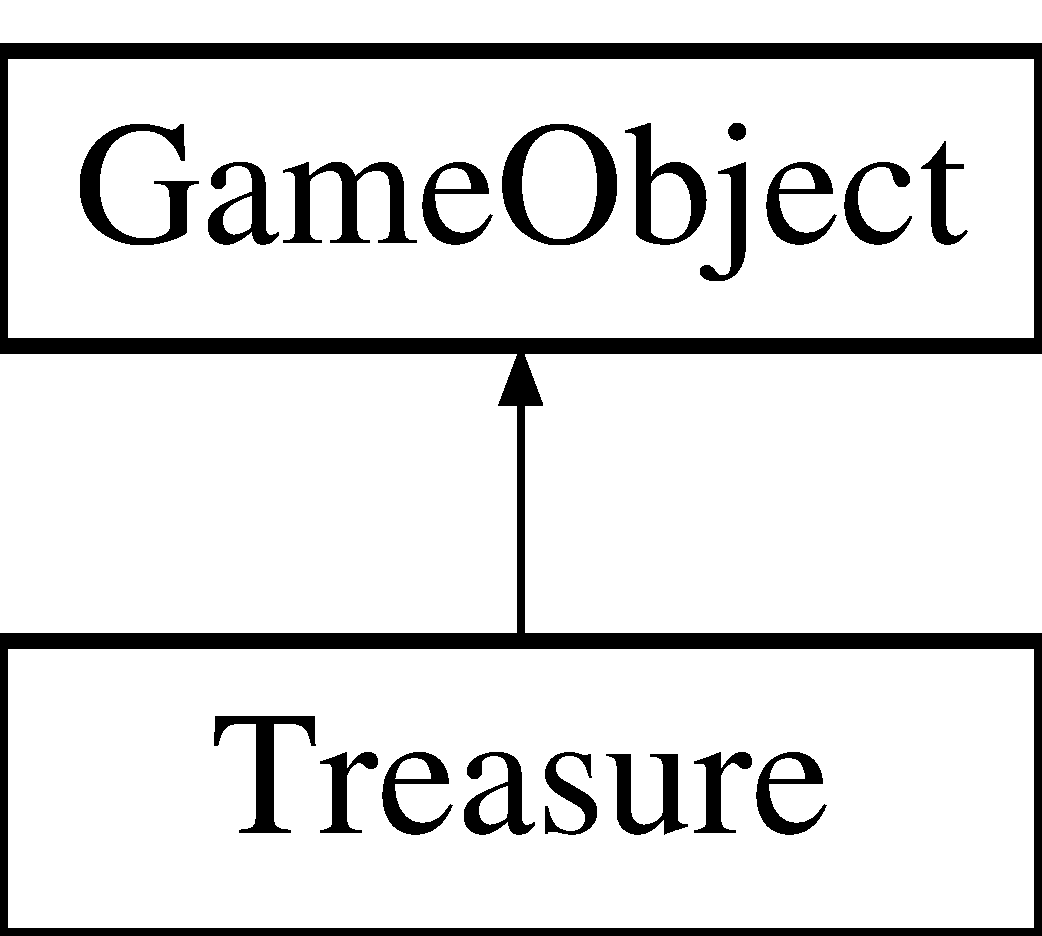
\includegraphics[height=2.000000cm]{classTreasure}
\end{center}
\end{figure}
\subsection*{\-Public \-Member \-Functions}
\begin{DoxyCompactItemize}
\item 
\hyperlink{classTreasure_a315282461bc05e7989fe6facbe6a1b43}{\-Treasure} (\-Scene\-Manager $\ast$)
\item 
virtual \-Game\-State \hyperlink{classTreasure_a31089b8e8c8478e7c3e950b80bdb3785}{frame\-Event\-Queued} (\hyperlink{classWayPoint}{\-Way\-Point} $\ast$current\-W\-P, \-Game\-State gs)
\item 
virtual void \hyperlink{classTreasure_a5fcd48652f78053fcb0c84e6a89415fe}{init} (\hyperlink{classRoom}{\-Room} $\ast$\hyperlink{classGameObject_a9f63419cc03f2513f757a317a2e37557}{room})
\end{DoxyCompactItemize}
\subsection*{\-Protected \-Member \-Functions}
\begin{DoxyCompactItemize}
\item 
\hyperlink{classTreasure_ac8a58fbc1d42bd355d9fdb2b5b8ba5e2}{\-Treasure} ()
\end{DoxyCompactItemize}
\subsection*{\-Protected \-Attributes}
\begin{DoxyCompactItemize}
\item 
\-Particle\-System $\ast$ \hyperlink{classTreasure_a81c9f96d7d58e6181a2e1fef8e815c65}{gold}
\item 
\-Particle\-System $\ast$ \hyperlink{classTreasure_a03e1ea9a9e71f70f453b8bd7e46d5a02}{fireworks}
\end{DoxyCompactItemize}


\subsection{\-Detailed \-Description}
\-Describes the appearance and behaviour of a \hyperlink{classTreasure}{\-Treasure} in the \hyperlink{classGame}{\-Game}. \-This class is similar to the other \-Game\-Objects. 

\subsection{\-Constructor \& \-Destructor \-Documentation}
\hypertarget{classTreasure_ac8a58fbc1d42bd355d9fdb2b5b8ba5e2}{\index{\-Treasure@{\-Treasure}!\-Treasure@{\-Treasure}}
\index{\-Treasure@{\-Treasure}!Treasure@{\-Treasure}}
\subsubsection[{\-Treasure}]{\setlength{\rightskip}{0pt plus 5cm}{\bf \-Treasure\-::\-Treasure} (
\begin{DoxyParamCaption}
{}
\end{DoxyParamCaption}
)\hspace{0.3cm}{\ttfamily  \mbox{[}protected\mbox{]}}}}\label{classTreasure_ac8a58fbc1d42bd355d9fdb2b5b8ba5e2}
\-Default constructor. \-Not to be used outside class scope. \hypertarget{classTreasure_a315282461bc05e7989fe6facbe6a1b43}{\index{\-Treasure@{\-Treasure}!\-Treasure@{\-Treasure}}
\index{\-Treasure@{\-Treasure}!Treasure@{\-Treasure}}
\subsubsection[{\-Treasure}]{\setlength{\rightskip}{0pt plus 5cm}{\bf \-Treasure\-::\-Treasure} (
\begin{DoxyParamCaption}
\item[{\-Scene\-Manager $\ast$}]{}
\end{DoxyParamCaption}
)}}\label{classTreasure_a315282461bc05e7989fe6facbe6a1b43}
\-Initialize the \hyperlink{classTreasure}{\-Treasure} object with the scene manager for object creation. 

\subsection{\-Member \-Function \-Documentation}
\hypertarget{classTreasure_a31089b8e8c8478e7c3e950b80bdb3785}{\index{\-Treasure@{\-Treasure}!frame\-Event\-Queued@{frame\-Event\-Queued}}
\index{frame\-Event\-Queued@{frame\-Event\-Queued}!Treasure@{\-Treasure}}
\subsubsection[{frame\-Event\-Queued}]{\setlength{\rightskip}{0pt plus 5cm}virtual \-Game\-State {\bf \-Treasure\-::frame\-Event\-Queued} (
\begin{DoxyParamCaption}
\item[{{\bf \-Way\-Point} $\ast$}]{current\-W\-P, }
\item[{\-Game\-State}]{gs}
\end{DoxyParamCaption}
)\hspace{0.3cm}{\ttfamily  \mbox{[}virtual\mbox{]}}}}\label{classTreasure_a31089b8e8c8478e7c3e950b80bdb3785}
\-Process the current robot \hyperlink{classWayPoint}{\-Way\-Point} and \-Game\-State for the \hyperlink{classTreasure}{\-Treasure} behaviour. 

\-Reimplemented from \hyperlink{classGameObject_aa643df342c50df77f053eee2c703c619}{\-Game\-Object}.

\hypertarget{classTreasure_a5fcd48652f78053fcb0c84e6a89415fe}{\index{\-Treasure@{\-Treasure}!init@{init}}
\index{init@{init}!Treasure@{\-Treasure}}
\subsubsection[{init}]{\setlength{\rightskip}{0pt plus 5cm}virtual void {\bf \-Treasure\-::init} (
\begin{DoxyParamCaption}
\item[{{\bf \-Room} $\ast$}]{room}
\end{DoxyParamCaption}
)\hspace{0.3cm}{\ttfamily  \mbox{[}virtual\mbox{]}}}}\label{classTreasure_a5fcd48652f78053fcb0c84e6a89415fe}
(\-Re)initialize the treasure for a new game session. 

\-Reimplemented from \hyperlink{classGameObject_ac3ab6708ce47b4ef8fd35d8bb43149dc}{\-Game\-Object}.



\subsection{\-Member \-Data \-Documentation}
\hypertarget{classTreasure_a03e1ea9a9e71f70f453b8bd7e46d5a02}{\index{\-Treasure@{\-Treasure}!fireworks@{fireworks}}
\index{fireworks@{fireworks}!Treasure@{\-Treasure}}
\subsubsection[{fireworks}]{\setlength{\rightskip}{0pt plus 5cm}\-Particle\-System $\ast$ {\bf \-Treasure\-::fireworks}\hspace{0.3cm}{\ttfamily  \mbox{[}protected\mbox{]}}}}\label{classTreasure_a03e1ea9a9e71f70f453b8bd7e46d5a02}
\-Fireworks as eye-\/candy, when the treasure is found. \hypertarget{classTreasure_a81c9f96d7d58e6181a2e1fef8e815c65}{\index{\-Treasure@{\-Treasure}!gold@{gold}}
\index{gold@{gold}!Treasure@{\-Treasure}}
\subsubsection[{gold}]{\setlength{\rightskip}{0pt plus 5cm}\-Particle\-System$\ast$ {\bf \-Treasure\-::gold}\hspace{0.3cm}{\ttfamily  \mbox{[}protected\mbox{]}}}}\label{classTreasure_a81c9f96d7d58e6181a2e1fef8e815c65}
\-Sparkling particle effect as eye-\/candy when the treasure is found. 

\-The documentation for this class was generated from the following file\-:\begin{DoxyCompactItemize}
\item 
roculus/include/\-Treasure.\-h\end{DoxyCompactItemize}

\hypertarget{classVideo3D}{\section{\-Video3\-D \-Class \-Reference}
\label{classVideo3D}\index{\-Video3\-D@{\-Video3\-D}}
}


\-Handles the 3\-D video stream. \-Similar to a \hyperlink{classSnapshot}{\-Snapshot}, but uses \-D\-Y\-N\-A\-M\-I\-C and \-D\-I\-S\-C\-A\-R\-D\-A\-B\-L\-E textures instead, which are updated, not placed. (\-Not the smartest implementation, should probably be inherit properties from \hyperlink{classSnapshot}{\-Snapshot}...)  




{\ttfamily \#include $<$\-Video3\-D.\-h$>$}

\subsection*{\-Public \-Member \-Functions}
\begin{DoxyCompactItemize}
\item 
\hyperlink{classVideo3D_aad8f80b8d60351bb34955a19c3f36d9b}{\-Video3\-D} (\-Ogre\-::\-Entity $\ast$, \-Ogre\-::\-Scene\-Node $\ast$, const \-Ogre\-::\-Texture\-Ptr \&, const \-Ogre\-::\-Texture\-Ptr \&)
\item 
\hyperlink{classVideo3D_a04f3933f882ba5f2e4fc36094e41abcf}{$\sim$\-Video3\-D} ()
\item 
virtual \-Ogre\-::\-Scene\-Node $\ast$ \hyperlink{classVideo3D_a19bafff8518433c46bb75cb9961fb8d6}{get\-Target\-Scene\-Node} ()
\item 
virtual \-Ogre\-::\-Texture\-Ptr \hyperlink{classVideo3D_aa1545fe5f983c6f9c51d43137b42b376}{get\-Assigned\-Depth\-Texture} ()
\item 
virtual \-Ogre\-::\-Texture\-Ptr \hyperlink{classVideo3D_a518e4f0e0cd61d33c55aad6a4ac17026}{get\-Assigned\-R\-G\-B\-Texture} ()
\item 
virtual void \hyperlink{classVideo3D_a1f2dc38dc3eee1286a550e97ce1685ec}{set\-Target\-Scene\-Node} (\-Ogre\-::\-Scene\-Node $\ast$)
\item 
virtual void \hyperlink{classVideo3D_a0be3f2fb99f5bba139d624077a55d640}{assign\-Depth\-Texture} (const \-Ogre\-::\-Texture\-Ptr \&)
\item 
virtual void \hyperlink{classVideo3D_a805bc17368571ce3826e98d45531cd2c}{assign\-R\-G\-B\-Texture} (const \-Ogre\-::\-Texture\-Ptr \&)
\item 
virtual bool \hyperlink{classVideo3D_a537270e52644622719f8765b86b00ec8}{update} (const \-Ogre\-::\-Image \&, const \-Ogre\-::\-Image \&, const \-Ogre\-::\-Vector3 \&, const \-Ogre\-::\-Quaternion \&)
\end{DoxyCompactItemize}
\subsection*{\-Protected \-Attributes}
\begin{DoxyCompactItemize}
\item 
\-Ogre\-::\-Entity $\ast$ \hyperlink{classVideo3D_ab8d19ec21e20d8e4fcb921db1f05c96e}{snapshot}
\item 
\-Ogre\-::\-Texture\-Ptr \hyperlink{classVideo3D_a1e9d633a5ac0c2b2468611190c2bba12}{depth\-Texture}
\item 
\-Ogre\-::\-Texture\-Ptr \hyperlink{classVideo3D_ae6ddba8b94b5f01dc4761255fcffdf81}{rgb\-Texture}
\item 
\-Ogre\-::\-Scene\-Node $\ast$ \hyperlink{classVideo3D_ab3e0e29264b1e813c3075bc0d562a2e8}{target\-Scene\-Node}
\item 
bool \hyperlink{classVideo3D_a4dc5c42b3005ccf0e6e9cffd26a6351d}{attached}
\end{DoxyCompactItemize}


\subsection{\-Detailed \-Description}
\-Handles the 3\-D video stream. \-Similar to a \hyperlink{classSnapshot}{\-Snapshot}, but uses \-D\-Y\-N\-A\-M\-I\-C and \-D\-I\-S\-C\-A\-R\-D\-A\-B\-L\-E textures instead, which are updated, not placed. (\-Not the smartest implementation, should probably be inherit properties from \hyperlink{classSnapshot}{\-Snapshot}...) 

\subsection{\-Constructor \& \-Destructor \-Documentation}
\hypertarget{classVideo3D_aad8f80b8d60351bb34955a19c3f36d9b}{\index{\-Video3\-D@{\-Video3\-D}!\-Video3\-D@{\-Video3\-D}}
\index{\-Video3\-D@{\-Video3\-D}!Video3D@{\-Video3\-D}}
\subsubsection[{\-Video3\-D}]{\setlength{\rightskip}{0pt plus 5cm}{\bf \-Video3\-D\-::\-Video3\-D} (
\begin{DoxyParamCaption}
\item[{\-Ogre\-::\-Entity $\ast$}]{, }
\item[{\-Ogre\-::\-Scene\-Node $\ast$}]{, }
\item[{const \-Ogre\-::\-Texture\-Ptr \&}]{, }
\item[{const \-Ogre\-::\-Texture\-Ptr \&}]{}
\end{DoxyParamCaption}
)}}\label{classVideo3D_aad8f80b8d60351bb34955a19c3f36d9b}
\-See constructor of \hyperlink{classSnapshot}{\-Snapshot} class. \hypertarget{classVideo3D_a04f3933f882ba5f2e4fc36094e41abcf}{\index{\-Video3\-D@{\-Video3\-D}!$\sim$\-Video3\-D@{$\sim$\-Video3\-D}}
\index{$\sim$\-Video3\-D@{$\sim$\-Video3\-D}!Video3D@{\-Video3\-D}}
\subsubsection[{$\sim$\-Video3\-D}]{\setlength{\rightskip}{0pt plus 5cm}{\bf \-Video3\-D\-::$\sim$\-Video3\-D} (
\begin{DoxyParamCaption}
{}
\end{DoxyParamCaption}
)}}\label{classVideo3D_a04f3933f882ba5f2e4fc36094e41abcf}
\-Default destructor. 

\subsection{\-Member \-Function \-Documentation}
\hypertarget{classVideo3D_a0be3f2fb99f5bba139d624077a55d640}{\index{\-Video3\-D@{\-Video3\-D}!assign\-Depth\-Texture@{assign\-Depth\-Texture}}
\index{assign\-Depth\-Texture@{assign\-Depth\-Texture}!Video3D@{\-Video3\-D}}
\subsubsection[{assign\-Depth\-Texture}]{\setlength{\rightskip}{0pt plus 5cm}virtual void {\bf \-Video3\-D\-::assign\-Depth\-Texture} (
\begin{DoxyParamCaption}
\item[{const \-Ogre\-::\-Texture\-Ptr \&}]{}
\end{DoxyParamCaption}
)\hspace{0.3cm}{\ttfamily  \mbox{[}virtual\mbox{]}}}}\label{classVideo3D_a0be3f2fb99f5bba139d624077a55d640}
\-Assign a depth texture. \hypertarget{classVideo3D_a805bc17368571ce3826e98d45531cd2c}{\index{\-Video3\-D@{\-Video3\-D}!assign\-R\-G\-B\-Texture@{assign\-R\-G\-B\-Texture}}
\index{assign\-R\-G\-B\-Texture@{assign\-R\-G\-B\-Texture}!Video3D@{\-Video3\-D}}
\subsubsection[{assign\-R\-G\-B\-Texture}]{\setlength{\rightskip}{0pt plus 5cm}virtual void {\bf \-Video3\-D\-::assign\-R\-G\-B\-Texture} (
\begin{DoxyParamCaption}
\item[{const \-Ogre\-::\-Texture\-Ptr \&}]{}
\end{DoxyParamCaption}
)\hspace{0.3cm}{\ttfamily  \mbox{[}virtual\mbox{]}}}}\label{classVideo3D_a805bc17368571ce3826e98d45531cd2c}
\-Assign a rgb texture. \hypertarget{classVideo3D_aa1545fe5f983c6f9c51d43137b42b376}{\index{\-Video3\-D@{\-Video3\-D}!get\-Assigned\-Depth\-Texture@{get\-Assigned\-Depth\-Texture}}
\index{get\-Assigned\-Depth\-Texture@{get\-Assigned\-Depth\-Texture}!Video3D@{\-Video3\-D}}
\subsubsection[{get\-Assigned\-Depth\-Texture}]{\setlength{\rightskip}{0pt plus 5cm}virtual \-Ogre\-::\-Texture\-Ptr {\bf \-Video3\-D\-::get\-Assigned\-Depth\-Texture} (
\begin{DoxyParamCaption}
{}
\end{DoxyParamCaption}
)\hspace{0.3cm}{\ttfamily  \mbox{[}virtual\mbox{]}}}}\label{classVideo3D_aa1545fe5f983c6f9c51d43137b42b376}
\-Get tointer to the depth texture of the 3\-D stream. \hypertarget{classVideo3D_a518e4f0e0cd61d33c55aad6a4ac17026}{\index{\-Video3\-D@{\-Video3\-D}!get\-Assigned\-R\-G\-B\-Texture@{get\-Assigned\-R\-G\-B\-Texture}}
\index{get\-Assigned\-R\-G\-B\-Texture@{get\-Assigned\-R\-G\-B\-Texture}!Video3D@{\-Video3\-D}}
\subsubsection[{get\-Assigned\-R\-G\-B\-Texture}]{\setlength{\rightskip}{0pt plus 5cm}virtual \-Ogre\-::\-Texture\-Ptr {\bf \-Video3\-D\-::get\-Assigned\-R\-G\-B\-Texture} (
\begin{DoxyParamCaption}
{}
\end{DoxyParamCaption}
)\hspace{0.3cm}{\ttfamily  \mbox{[}virtual\mbox{]}}}}\label{classVideo3D_a518e4f0e0cd61d33c55aad6a4ac17026}
\-Get the pointer to the rgb texture of the stream. \hypertarget{classVideo3D_a19bafff8518433c46bb75cb9961fb8d6}{\index{\-Video3\-D@{\-Video3\-D}!get\-Target\-Scene\-Node@{get\-Target\-Scene\-Node}}
\index{get\-Target\-Scene\-Node@{get\-Target\-Scene\-Node}!Video3D@{\-Video3\-D}}
\subsubsection[{get\-Target\-Scene\-Node}]{\setlength{\rightskip}{0pt plus 5cm}virtual \-Ogre\-::\-Scene\-Node$\ast$ {\bf \-Video3\-D\-::get\-Target\-Scene\-Node} (
\begin{DoxyParamCaption}
{}
\end{DoxyParamCaption}
)\hspace{0.3cm}{\ttfamily  \mbox{[}virtual\mbox{]}}}}\label{classVideo3D_a19bafff8518433c46bb75cb9961fb8d6}
\-The scene node of the video stream. \hypertarget{classVideo3D_a1f2dc38dc3eee1286a550e97ce1685ec}{\index{\-Video3\-D@{\-Video3\-D}!set\-Target\-Scene\-Node@{set\-Target\-Scene\-Node}}
\index{set\-Target\-Scene\-Node@{set\-Target\-Scene\-Node}!Video3D@{\-Video3\-D}}
\subsubsection[{set\-Target\-Scene\-Node}]{\setlength{\rightskip}{0pt plus 5cm}virtual void {\bf \-Video3\-D\-::set\-Target\-Scene\-Node} (
\begin{DoxyParamCaption}
\item[{\-Ogre\-::\-Scene\-Node $\ast$}]{}
\end{DoxyParamCaption}
)\hspace{0.3cm}{\ttfamily  \mbox{[}virtual\mbox{]}}}}\label{classVideo3D_a1f2dc38dc3eee1286a550e97ce1685ec}
\-Set the scene node. (\-Not used, done during construction. \hypertarget{classVideo3D_a537270e52644622719f8765b86b00ec8}{\index{\-Video3\-D@{\-Video3\-D}!update@{update}}
\index{update@{update}!Video3D@{\-Video3\-D}}
\subsubsection[{update}]{\setlength{\rightskip}{0pt plus 5cm}virtual bool {\bf \-Video3\-D\-::update} (
\begin{DoxyParamCaption}
\item[{const \-Ogre\-::\-Image \&}]{, }
\item[{const \-Ogre\-::\-Image \&}]{, }
\item[{const \-Ogre\-::\-Vector3 \&}]{, }
\item[{const \-Ogre\-::\-Quaternion \&}]{}
\end{DoxyParamCaption}
)\hspace{0.3cm}{\ttfamily  \mbox{[}virtual\mbox{]}}}}\label{classVideo3D_a537270e52644622719f8765b86b00ec8}
\-Update the video stream with the new\-: (1) depth image, (2) rgb image, (3) position and (4) orientation. 

\subsection{\-Member \-Data \-Documentation}
\hypertarget{classVideo3D_a4dc5c42b3005ccf0e6e9cffd26a6351d}{\index{\-Video3\-D@{\-Video3\-D}!attached@{attached}}
\index{attached@{attached}!Video3D@{\-Video3\-D}}
\subsubsection[{attached}]{\setlength{\rightskip}{0pt plus 5cm}bool {\bf \-Video3\-D\-::attached}\hspace{0.3cm}{\ttfamily  \mbox{[}protected\mbox{]}}}}\label{classVideo3D_a4dc5c42b3005ccf0e6e9cffd26a6351d}
\-Was this object already attached to its scene node? \hypertarget{classVideo3D_a1e9d633a5ac0c2b2468611190c2bba12}{\index{\-Video3\-D@{\-Video3\-D}!depth\-Texture@{depth\-Texture}}
\index{depth\-Texture@{depth\-Texture}!Video3D@{\-Video3\-D}}
\subsubsection[{depth\-Texture}]{\setlength{\rightskip}{0pt plus 5cm}\-Ogre\-::\-Texture\-Ptr {\bf \-Video3\-D\-::depth\-Texture}\hspace{0.3cm}{\ttfamily  \mbox{[}protected\mbox{]}}}}\label{classVideo3D_a1e9d633a5ac0c2b2468611190c2bba12}
\-Pointer to the depth texture. \hypertarget{classVideo3D_ae6ddba8b94b5f01dc4761255fcffdf81}{\index{\-Video3\-D@{\-Video3\-D}!rgb\-Texture@{rgb\-Texture}}
\index{rgb\-Texture@{rgb\-Texture}!Video3D@{\-Video3\-D}}
\subsubsection[{rgb\-Texture}]{\setlength{\rightskip}{0pt plus 5cm}\-Ogre\-::\-Texture\-Ptr {\bf \-Video3\-D\-::rgb\-Texture}\hspace{0.3cm}{\ttfamily  \mbox{[}protected\mbox{]}}}}\label{classVideo3D_ae6ddba8b94b5f01dc4761255fcffdf81}
\-Pointer to the rgb texture. \hypertarget{classVideo3D_ab8d19ec21e20d8e4fcb921db1f05c96e}{\index{\-Video3\-D@{\-Video3\-D}!snapshot@{snapshot}}
\index{snapshot@{snapshot}!Video3D@{\-Video3\-D}}
\subsubsection[{snapshot}]{\setlength{\rightskip}{0pt plus 5cm}\-Ogre\-::\-Entity$\ast$ {\bf \-Video3\-D\-::snapshot}\hspace{0.3cm}{\ttfamily  \mbox{[}protected\mbox{]}}}}\label{classVideo3D_ab8d19ec21e20d8e4fcb921db1f05c96e}
\-The entity of the video. \hypertarget{classVideo3D_ab3e0e29264b1e813c3075bc0d562a2e8}{\index{\-Video3\-D@{\-Video3\-D}!target\-Scene\-Node@{target\-Scene\-Node}}
\index{target\-Scene\-Node@{target\-Scene\-Node}!Video3D@{\-Video3\-D}}
\subsubsection[{target\-Scene\-Node}]{\setlength{\rightskip}{0pt plus 5cm}\-Ogre\-::\-Scene\-Node$\ast$ {\bf \-Video3\-D\-::target\-Scene\-Node}\hspace{0.3cm}{\ttfamily  \mbox{[}protected\mbox{]}}}}\label{classVideo3D_ab3e0e29264b1e813c3075bc0d562a2e8}
\-The scene node of the video. 

\-The documentation for this class was generated from the following file\-:\begin{DoxyCompactItemize}
\item 
roculus/include/\-Video3\-D.\-h\end{DoxyCompactItemize}

\hypertarget{classWayPoint}{\section{\-Way\-Point \-Class \-Reference}
\label{classWayPoint}\index{\-Way\-Point@{\-Way\-Point}}
}


\-Defines a \hyperlink{classWayPoint}{\-Way\-Point} for the \hyperlink{classGame}{\-Game}. \-Waypoints are possible navigation targets and are used to place \-Game\-Objects, like \-Keys and \-Locks. \-The list of \-Way\-Points is held by the \hyperlink{classGame}{\-Game} class, but they are read from other classes quite often, usually passed as a pointer or reference. \-A \hyperlink{classWayPoint}{\-Way\-Point} can be made inaccessible for the selection by the player setting the accessible flag.  




{\ttfamily \#include $<$\-Way\-Point.\-h$>$}

\subsection*{\-Public \-Member \-Functions}
\begin{DoxyCompactItemize}
\item 
\hyperlink{classWayPoint_a13644b20d0bf0ae35a3f0919b67f65aa}{\-Way\-Point} (int, \-Scene\-Manager $\ast$, \-Vector3, \-Quaternion, \-Way\-Point\-\_\-\-Role)
\item 
\-String \hyperlink{classWayPoint_afcbd6e620869ab00a36a36ac63d41e1a}{get\-Name} ()
\item 
const \-Vector3 \& \hyperlink{classWayPoint_a79327a4ecc81d6cabd5be1ea553474e3}{get\-Position} ()
\item 
const \-Quaternion \& \hyperlink{classWayPoint_aa89f93715f369c3be302b1c416ba5421}{get\-Orientation} ()
\item 
int \hyperlink{classWayPoint_a2c2c44621b047d3bdfdf4f0ee7e2566e}{get\-Id} ()
\item 
\-Way\-Point\-\_\-\-Role \hyperlink{classWayPoint_a52fd4b22dc0db0454ba891c799f1220c}{get\-Role} ()
\item 
void \hyperlink{classWayPoint_a6603a3e2950050021fb2af4f19b9cea1}{set\-Role} (\-Way\-Point\-\_\-\-Role \hyperlink{classWayPoint_aed5b54453c7dc642ee8125158942ccd0}{role})
\item 
void \hyperlink{classWayPoint_a58f2d2b3cf03026c34dc6cae2dbcf24e}{set\-Position} (const \-Vector3 \&\hyperlink{classWayPoint_aaace5c39e2b733295ef37de4228eb115}{pos})
\item 
void \hyperlink{classWayPoint_aef37a4697991dddae64f6b2bd7c1eb67}{set\-Orientation} (const \-Quaternion \&orientation)
\item 
bool \hyperlink{classWayPoint_aa6ea489c68a04bc8b4bbce8f30d470f4}{is\-Accessible} ()
\item 
void \hyperlink{classWayPoint_aaec82ed4514b47784e9e44b2becf8fc4}{set\-Accessibility} (bool)
\item 
void \hyperlink{classWayPoint_a7c3744470bb0733a8d027203def48925}{set\-Visible} (bool visible)
\item 
std\-::string \hyperlink{classWayPoint_adbda23a7d37cec525bd40e317c134b92}{to\-String} ()
\end{DoxyCompactItemize}
\subsection*{\-Protected \-Attributes}
\begin{DoxyCompactItemize}
\item 
boost\-::mutex \hyperlink{classWayPoint_ac889b89eb8c36244c7b937bed5c2d77e}{\-W\-A\-Y\-P\-O\-I\-N\-T\-\_\-\-M\-U\-T\-E\-X}
\item 
int \hyperlink{classWayPoint_a01b5cf642bf27270f3eb44adfe7de271}{id}
\item 
\-Scene\-Manager $\ast$ \hyperlink{classWayPoint_a8a18ed96355454b4f1713d196aff2216}{m\-Scene\-Mgr}
\item 
\-Scene\-Node $\ast$ \hyperlink{classWayPoint_aeb4358a9171b219b8f0281cf84b5b6e0}{wp\-S\-N}
\item 
\-Entity $\ast$ \hyperlink{classWayPoint_a604e3fa32b79b6e2c9fabcf321f7c774}{wp\-Ent}
\item 
\-String \hyperlink{classWayPoint_aca34a5b321d0f27d810a3097c3ef0f3a}{name}
\item 
\-Vector3 \hyperlink{classWayPoint_aaace5c39e2b733295ef37de4228eb115}{pos}
\item 
\-Quaternion \hyperlink{classWayPoint_a5335f01d55f54a40acf21fa25d93efc0}{ori}
\item 
\-Way\-Point\-\_\-\-Role \hyperlink{classWayPoint_aed5b54453c7dc642ee8125158942ccd0}{role}
\item 
bool \hyperlink{classWayPoint_aae4377ca4bb86993f6572403e1d7e71c}{accessible}
\end{DoxyCompactItemize}


\subsection{\-Detailed \-Description}
\-Defines a \hyperlink{classWayPoint}{\-Way\-Point} for the \hyperlink{classGame}{\-Game}. \-Waypoints are possible navigation targets and are used to place \-Game\-Objects, like \-Keys and \-Locks. \-The list of \-Way\-Points is held by the \hyperlink{classGame}{\-Game} class, but they are read from other classes quite often, usually passed as a pointer or reference. \-A \hyperlink{classWayPoint}{\-Way\-Point} can be made inaccessible for the selection by the player setting the accessible flag. 

\subsection{\-Constructor \& \-Destructor \-Documentation}
\hypertarget{classWayPoint_a13644b20d0bf0ae35a3f0919b67f65aa}{\index{\-Way\-Point@{\-Way\-Point}!\-Way\-Point@{\-Way\-Point}}
\index{\-Way\-Point@{\-Way\-Point}!WayPoint@{\-Way\-Point}}
\subsubsection[{\-Way\-Point}]{\setlength{\rightskip}{0pt plus 5cm}{\bf \-Way\-Point\-::\-Way\-Point} (
\begin{DoxyParamCaption}
\item[{int}]{, }
\item[{\-Scene\-Manager $\ast$}]{, }
\item[{\-Vector3}]{, }
\item[{\-Quaternion}]{, }
\item[{\-Way\-Point\-\_\-\-Role}]{}
\end{DoxyParamCaption}
)}}\label{classWayPoint_a13644b20d0bf0ae35a3f0919b67f65aa}
\-Initialize a \hyperlink{classWayPoint}{\-Way\-Point} with\-: (1) a unique \-I\-D, (2) the scene manager, (3) the position and (4) its role. 

\subsection{\-Member \-Function \-Documentation}
\hypertarget{classWayPoint_a2c2c44621b047d3bdfdf4f0ee7e2566e}{\index{\-Way\-Point@{\-Way\-Point}!get\-Id@{get\-Id}}
\index{get\-Id@{get\-Id}!WayPoint@{\-Way\-Point}}
\subsubsection[{get\-Id}]{\setlength{\rightskip}{0pt plus 5cm}int {\bf \-Way\-Point\-::get\-Id} (
\begin{DoxyParamCaption}
{}
\end{DoxyParamCaption}
)}}\label{classWayPoint_a2c2c44621b047d3bdfdf4f0ee7e2566e}
\-Returns the \-I\-D of this waypoint. \hypertarget{classWayPoint_afcbd6e620869ab00a36a36ac63d41e1a}{\index{\-Way\-Point@{\-Way\-Point}!get\-Name@{get\-Name}}
\index{get\-Name@{get\-Name}!WayPoint@{\-Way\-Point}}
\subsubsection[{get\-Name}]{\setlength{\rightskip}{0pt plus 5cm}\-String {\bf \-Way\-Point\-::get\-Name} (
\begin{DoxyParamCaption}
{}
\end{DoxyParamCaption}
)}}\label{classWayPoint_afcbd6e620869ab00a36a36ac63d41e1a}
\-Returns the name of this waypoint. \hypertarget{classWayPoint_aa89f93715f369c3be302b1c416ba5421}{\index{\-Way\-Point@{\-Way\-Point}!get\-Orientation@{get\-Orientation}}
\index{get\-Orientation@{get\-Orientation}!WayPoint@{\-Way\-Point}}
\subsubsection[{get\-Orientation}]{\setlength{\rightskip}{0pt plus 5cm}const \-Quaternion\& {\bf \-Way\-Point\-::get\-Orientation} (
\begin{DoxyParamCaption}
{}
\end{DoxyParamCaption}
)}}\label{classWayPoint_aa89f93715f369c3be302b1c416ba5421}
\-Returns the orientation of this waypoint. \hypertarget{classWayPoint_a79327a4ecc81d6cabd5be1ea553474e3}{\index{\-Way\-Point@{\-Way\-Point}!get\-Position@{get\-Position}}
\index{get\-Position@{get\-Position}!WayPoint@{\-Way\-Point}}
\subsubsection[{get\-Position}]{\setlength{\rightskip}{0pt plus 5cm}const \-Vector3\& {\bf \-Way\-Point\-::get\-Position} (
\begin{DoxyParamCaption}
{}
\end{DoxyParamCaption}
)}}\label{classWayPoint_a79327a4ecc81d6cabd5be1ea553474e3}
\-Returns the position of this waypoint. \hypertarget{classWayPoint_a52fd4b22dc0db0454ba891c799f1220c}{\index{\-Way\-Point@{\-Way\-Point}!get\-Role@{get\-Role}}
\index{get\-Role@{get\-Role}!WayPoint@{\-Way\-Point}}
\subsubsection[{get\-Role}]{\setlength{\rightskip}{0pt plus 5cm}\-Way\-Point\-\_\-\-Role {\bf \-Way\-Point\-::get\-Role} (
\begin{DoxyParamCaption}
{}
\end{DoxyParamCaption}
)}}\label{classWayPoint_a52fd4b22dc0db0454ba891c799f1220c}
\-Returns the role of this waypoint. \hypertarget{classWayPoint_aa6ea489c68a04bc8b4bbce8f30d470f4}{\index{\-Way\-Point@{\-Way\-Point}!is\-Accessible@{is\-Accessible}}
\index{is\-Accessible@{is\-Accessible}!WayPoint@{\-Way\-Point}}
\subsubsection[{is\-Accessible}]{\setlength{\rightskip}{0pt plus 5cm}bool {\bf \-Way\-Point\-::is\-Accessible} (
\begin{DoxyParamCaption}
{}
\end{DoxyParamCaption}
)}}\label{classWayPoint_aa6ea489c68a04bc8b4bbce8f30d470f4}
\-Can this waypoint currently be a navigation target? \hypertarget{classWayPoint_aaec82ed4514b47784e9e44b2becf8fc4}{\index{\-Way\-Point@{\-Way\-Point}!set\-Accessibility@{set\-Accessibility}}
\index{set\-Accessibility@{set\-Accessibility}!WayPoint@{\-Way\-Point}}
\subsubsection[{set\-Accessibility}]{\setlength{\rightskip}{0pt plus 5cm}void {\bf \-Way\-Point\-::set\-Accessibility} (
\begin{DoxyParamCaption}
\item[{bool}]{}
\end{DoxyParamCaption}
)}}\label{classWayPoint_aaec82ed4514b47784e9e44b2becf8fc4}
\-Set the accessibility of this waypoint (true means accessible). \hypertarget{classWayPoint_aef37a4697991dddae64f6b2bd7c1eb67}{\index{\-Way\-Point@{\-Way\-Point}!set\-Orientation@{set\-Orientation}}
\index{set\-Orientation@{set\-Orientation}!WayPoint@{\-Way\-Point}}
\subsubsection[{set\-Orientation}]{\setlength{\rightskip}{0pt plus 5cm}void {\bf \-Way\-Point\-::set\-Orientation} (
\begin{DoxyParamCaption}
\item[{const \-Quaternion \&}]{orientation}
\end{DoxyParamCaption}
)}}\label{classWayPoint_aef37a4697991dddae64f6b2bd7c1eb67}
\-Sets the orientation of this waypoint. \hypertarget{classWayPoint_a58f2d2b3cf03026c34dc6cae2dbcf24e}{\index{\-Way\-Point@{\-Way\-Point}!set\-Position@{set\-Position}}
\index{set\-Position@{set\-Position}!WayPoint@{\-Way\-Point}}
\subsubsection[{set\-Position}]{\setlength{\rightskip}{0pt plus 5cm}void {\bf \-Way\-Point\-::set\-Position} (
\begin{DoxyParamCaption}
\item[{const \-Vector3 \&}]{pos}
\end{DoxyParamCaption}
)}}\label{classWayPoint_a58f2d2b3cf03026c34dc6cae2dbcf24e}
\-Sets the position of this waypoint. \hypertarget{classWayPoint_a6603a3e2950050021fb2af4f19b9cea1}{\index{\-Way\-Point@{\-Way\-Point}!set\-Role@{set\-Role}}
\index{set\-Role@{set\-Role}!WayPoint@{\-Way\-Point}}
\subsubsection[{set\-Role}]{\setlength{\rightskip}{0pt plus 5cm}void {\bf \-Way\-Point\-::set\-Role} (
\begin{DoxyParamCaption}
\item[{\-Way\-Point\-\_\-\-Role}]{role}
\end{DoxyParamCaption}
)}}\label{classWayPoint_a6603a3e2950050021fb2af4f19b9cea1}
\-Sets the role of this waypoint. \hypertarget{classWayPoint_a7c3744470bb0733a8d027203def48925}{\index{\-Way\-Point@{\-Way\-Point}!set\-Visible@{set\-Visible}}
\index{set\-Visible@{set\-Visible}!WayPoint@{\-Way\-Point}}
\subsubsection[{set\-Visible}]{\setlength{\rightskip}{0pt plus 5cm}void {\bf \-Way\-Point\-::set\-Visible} (
\begin{DoxyParamCaption}
\item[{bool}]{visible}
\end{DoxyParamCaption}
)}}\label{classWayPoint_a7c3744470bb0733a8d027203def48925}
\-Set the visibility of this waypoint. \-Forwarded to the scene node. \hypertarget{classWayPoint_adbda23a7d37cec525bd40e317c134b92}{\index{\-Way\-Point@{\-Way\-Point}!to\-String@{to\-String}}
\index{to\-String@{to\-String}!WayPoint@{\-Way\-Point}}
\subsubsection[{to\-String}]{\setlength{\rightskip}{0pt plus 5cm}std\-::string {\bf \-Way\-Point\-::to\-String} (
\begin{DoxyParamCaption}
{}
\end{DoxyParamCaption}
)}}\label{classWayPoint_adbda23a7d37cec525bd40e317c134b92}
\-Return a string with the parameters of this waypoint. \-Useful for debugging. 

\subsection{\-Member \-Data \-Documentation}
\hypertarget{classWayPoint_aae4377ca4bb86993f6572403e1d7e71c}{\index{\-Way\-Point@{\-Way\-Point}!accessible@{accessible}}
\index{accessible@{accessible}!WayPoint@{\-Way\-Point}}
\subsubsection[{accessible}]{\setlength{\rightskip}{0pt plus 5cm}bool {\bf \-Way\-Point\-::accessible}\hspace{0.3cm}{\ttfamily  \mbox{[}protected\mbox{]}}}}\label{classWayPoint_aae4377ca4bb86993f6572403e1d7e71c}
\-Can this waypoint be targeted for navigation? \hypertarget{classWayPoint_a01b5cf642bf27270f3eb44adfe7de271}{\index{\-Way\-Point@{\-Way\-Point}!id@{id}}
\index{id@{id}!WayPoint@{\-Way\-Point}}
\subsubsection[{id}]{\setlength{\rightskip}{0pt plus 5cm}int {\bf \-Way\-Point\-::id}\hspace{0.3cm}{\ttfamily  \mbox{[}protected\mbox{]}}}}\label{classWayPoint_a01b5cf642bf27270f3eb44adfe7de271}
\-I\-D of this waypoint. \hypertarget{classWayPoint_a8a18ed96355454b4f1713d196aff2216}{\index{\-Way\-Point@{\-Way\-Point}!m\-Scene\-Mgr@{m\-Scene\-Mgr}}
\index{m\-Scene\-Mgr@{m\-Scene\-Mgr}!WayPoint@{\-Way\-Point}}
\subsubsection[{m\-Scene\-Mgr}]{\setlength{\rightskip}{0pt plus 5cm}\-Scene\-Manager$\ast$ {\bf \-Way\-Point\-::m\-Scene\-Mgr}\hspace{0.3cm}{\ttfamily  \mbox{[}protected\mbox{]}}}}\label{classWayPoint_a8a18ed96355454b4f1713d196aff2216}
\-Scene manager, to create the nodes/entities for display. \hypertarget{classWayPoint_aca34a5b321d0f27d810a3097c3ef0f3a}{\index{\-Way\-Point@{\-Way\-Point}!name@{name}}
\index{name@{name}!WayPoint@{\-Way\-Point}}
\subsubsection[{name}]{\setlength{\rightskip}{0pt plus 5cm}\-String {\bf \-Way\-Point\-::name}\hspace{0.3cm}{\ttfamily  \mbox{[}protected\mbox{]}}}}\label{classWayPoint_aca34a5b321d0f27d810a3097c3ef0f3a}
\-The name of the waypoint. \-Comform with the \-R\-O\-S notation \char`\"{}\-Way\-Point\char`\"{}.append(\#\-I\-D). \hypertarget{classWayPoint_a5335f01d55f54a40acf21fa25d93efc0}{\index{\-Way\-Point@{\-Way\-Point}!ori@{ori}}
\index{ori@{ori}!WayPoint@{\-Way\-Point}}
\subsubsection[{ori}]{\setlength{\rightskip}{0pt plus 5cm}\-Quaternion {\bf \-Way\-Point\-::ori}\hspace{0.3cm}{\ttfamily  \mbox{[}protected\mbox{]}}}}\label{classWayPoint_a5335f01d55f54a40acf21fa25d93efc0}
\-The orientation of this waypoint. \-If the waypoint is a navigation target, \-R\-O\-S\-I\-E will turn into this direction. \-If it is just a node in the path, it does not play a role. \hypertarget{classWayPoint_aaace5c39e2b733295ef37de4228eb115}{\index{\-Way\-Point@{\-Way\-Point}!pos@{pos}}
\index{pos@{pos}!WayPoint@{\-Way\-Point}}
\subsubsection[{pos}]{\setlength{\rightskip}{0pt plus 5cm}\-Vector3 {\bf \-Way\-Point\-::pos}\hspace{0.3cm}{\ttfamily  \mbox{[}protected\mbox{]}}}}\label{classWayPoint_aaace5c39e2b733295ef37de4228eb115}
\-The position of this waypoint. \hypertarget{classWayPoint_aed5b54453c7dc642ee8125158942ccd0}{\index{\-Way\-Point@{\-Way\-Point}!role@{role}}
\index{role@{role}!WayPoint@{\-Way\-Point}}
\subsubsection[{role}]{\setlength{\rightskip}{0pt plus 5cm}\-Way\-Point\-\_\-\-Role {\bf \-Way\-Point\-::role}\hspace{0.3cm}{\ttfamily  \mbox{[}protected\mbox{]}}}}\label{classWayPoint_aed5b54453c7dc642ee8125158942ccd0}
\-The role of this waypoint in the \hyperlink{classGame}{\-Game}. (\-Not in use). \hypertarget{classWayPoint_ac889b89eb8c36244c7b937bed5c2d77e}{\index{\-Way\-Point@{\-Way\-Point}!\-W\-A\-Y\-P\-O\-I\-N\-T\-\_\-\-M\-U\-T\-E\-X@{\-W\-A\-Y\-P\-O\-I\-N\-T\-\_\-\-M\-U\-T\-E\-X}}
\index{\-W\-A\-Y\-P\-O\-I\-N\-T\-\_\-\-M\-U\-T\-E\-X@{\-W\-A\-Y\-P\-O\-I\-N\-T\-\_\-\-M\-U\-T\-E\-X}!WayPoint@{\-Way\-Point}}
\subsubsection[{\-W\-A\-Y\-P\-O\-I\-N\-T\-\_\-\-M\-U\-T\-E\-X}]{\setlength{\rightskip}{0pt plus 5cm}boost\-::mutex {\bf \-Way\-Point\-::\-W\-A\-Y\-P\-O\-I\-N\-T\-\_\-\-M\-U\-T\-E\-X}\hspace{0.3cm}{\ttfamily  \mbox{[}protected\mbox{]}}}}\label{classWayPoint_ac889b89eb8c36244c7b937bed5c2d77e}
\-Mutex to ensure unique access to the waypoints. (\-Haven't really tested if this makes any difference). \hypertarget{classWayPoint_a604e3fa32b79b6e2c9fabcf321f7c774}{\index{\-Way\-Point@{\-Way\-Point}!wp\-Ent@{wp\-Ent}}
\index{wp\-Ent@{wp\-Ent}!WayPoint@{\-Way\-Point}}
\subsubsection[{wp\-Ent}]{\setlength{\rightskip}{0pt plus 5cm}\-Entity$\ast$ {\bf \-Way\-Point\-::wp\-Ent}\hspace{0.3cm}{\ttfamily  \mbox{[}protected\mbox{]}}}}\label{classWayPoint_a604e3fa32b79b6e2c9fabcf321f7c774}
\-The entity of this waypoint. \-Stored to be able to change the material (transparent if not accessible). \hypertarget{classWayPoint_aeb4358a9171b219b8f0281cf84b5b6e0}{\index{\-Way\-Point@{\-Way\-Point}!wp\-S\-N@{wp\-S\-N}}
\index{wp\-S\-N@{wp\-S\-N}!WayPoint@{\-Way\-Point}}
\subsubsection[{wp\-S\-N}]{\setlength{\rightskip}{0pt plus 5cm}\-Scene\-Node$\ast$ {\bf \-Way\-Point\-::wp\-S\-N}\hspace{0.3cm}{\ttfamily  \mbox{[}protected\mbox{]}}}}\label{classWayPoint_aeb4358a9171b219b8f0281cf84b5b6e0}
\-The scene node of this waypoint. 

\-The documentation for this class was generated from the following file\-:\begin{DoxyCompactItemize}
\item 
roculus/include/\-Way\-Point.\-h\end{DoxyCompactItemize}

\printindex
\end{document}
